% Initial and revised submissions should be 12 point; this will be removed in the final version.
\documentclass[12pt]{TD-CJS}

% Initial and revised submissions should also be double spaced.  This command will be removed in the final version.
\renewcommand{\baselinestretch}{2}

\usepackage{latexsym}
\usepackage{amsmath}
\usepackage{amsfonts}
\usepackage{amssymb}
\usepackage{psfrag}
\usepackage{graphicx}
\usepackage[dvipsnames]{xcolor}
\usepackage{url}
% header.tex
% this is where you load pacakges, specify custom formats, etc.

% \usepackage{changepage}
\usepackage{amsmath,amsthm,amssymb,amsfonts}
\usepackage{mathtools}
\usepackage{bbm}
% enumitem for custom lists
\usepackage{enumitem}
% Load dsfont this to get proper indicator function (bold 1) with \mathds{1}:
\usepackage{dsfont}
\usepackage{centernot}
\usepackage{appendix}

% set up graphics
\usepackage{graphicx}
\DeclareGraphicsExtensions{.pdf,.png,.jpg}
\graphicspath{ {fig/} }
% defs.tex
% this is where you define custom notation, commands, etc.

\DeclareMathOperator*{\argmax}{arg\,max}
\DeclareMathOperator*{\argmin}{arg\,min}
\DeclareMathOperator*{\del}{\nabla}

%%
% full alphabets of different styles
%%

% bf series
\def\bfA{\mathbf{A}}
\def\bfB{\mathbf{B}}
\def\bfC{\mathbf{C}}
\def\bfD{\mathbf{D}}
\def\bfE{\mathbf{E}}
\def\bfF{\mathbf{F}}
\def\bfG{\mathbf{G}}
\def\bfH{\mathbf{H}}
\def\bfI{\mathbf{I}}
\def\bfJ{\mathbf{J}}
\def\bfK{\mathbf{K}}
\def\bfL{\mathbf{L}}
\def\bfM{\mathbf{M}}
\def\bfN{\mathbf{N}}
\def\bfO{\mathbf{O}}
\def\bfP{\mathbf{P}}
\def\bfQ{\mathbf{Q}}
\def\bfR{\mathbf{R}}
\def\bfS{\mathbf{S}}
\def\bfT{\mathbf{T}}
\def\bfU{\mathbf{U}}
\def\bfV{\mathbf{V}}
\def\bfW{\mathbf{W}}
\def\bfX{\mathbf{X}}
\def\bfY{\mathbf{Y}}
\def\bfZ{\mathbf{Z}}

% bb series
\def\bbA{\mathbb{A}}
\def\bbB{\mathbb{B}}
\def\bbC{\mathbb{C}}
\def\bbD{\mathbb{D}}
\def\bbE{\mathbb{E}}
\def\bbF{\mathbb{F}}
\def\bbG{\mathbb{G}}
\def\bbH{\mathbb{H}}
\def\bbI{\mathbb{I}}
\def\bbJ{\mathbb{J}}
\def\bbK{\mathbb{K}}
\def\bbL{\mathbb{L}}
\def\bbM{\mathbb{M}}
\def\bbN{\mathbb{N}}
\def\bbO{\mathbb{O}}
\def\bbP{\mathbb{P}}
\def\bbQ{\mathbb{Q}}
\def\bbR{\mathbb{R}}
\def\bbS{\mathbb{S}}
\def\bbT{\mathbb{T}}
\def\bbU{\mathbb{U}}
\def\bbV{\mathbb{V}}
\def\bbW{\mathbb{W}}
\def\bbX{\mathbb{X}}
\def\bbY{\mathbb{Y}}
\def\bbZ{\mathbb{Z}}

% cal series
\def\calA{\mathcal{A}}
\def\calB{\mathcal{B}}
\def\calC{\mathcal{C}}
\def\calD{\mathcal{D}}
\def\calE{\mathcal{E}}
\def\calF{\mathcal{F}}
\def\calG{\mathcal{G}}
\def\calH{\mathcal{H}}
\def\calI{\mathcal{I}}
\def\calJ{\mathcal{J}}
\def\calK{\mathcal{K}}
\def\calL{\mathcal{L}}
\def\calM{\mathcal{M}}
\def\calN{\mathcal{N}}
\def\calO{\mathcal{O}}
\def\calP{\mathcal{P}}
\def\calQ{\mathcal{Q}}
\def\calR{\mathcal{R}}
\def\calS{\mathcal{S}}
\def\calT{\mathcal{T}}
\def\calU{\mathcal{U}}
\def\calV{\mathcal{V}}
\def\calW{\mathcal{W}}
\def\calX{\mathcal{X}}
\def\calY{\mathcal{Y}}
\def\calZ{\mathcal{Z}}

\def\bfTheta{\mathbf{\Theta}}


%%%%%%%%%%%%%%%%%%%%%%%%%%%%%%%%%%%%%%%%%%%%%%%%%%%%%%%%%%
% text short-cuts
\def\iid{i.i.d.\ } %i.i.d.
\def\ie{i.e.\ }
\def\eg{e.g.\ }
\def\Polya{P\'{o}lya\ }
%%%%%%%%%%%%%%%%%%%%%%%%%%%%%%%%%%%%%%%%%%%%%%%%%%%%%%%%%%

%%%%%%%%%%%%%%%%%%%%%%%%%%%%%%%%%%%%%%%%%%%%%%%%%%%%%%%%%%
% quasi-universal probabilistic and mathematical notation
% my preferences (modulo publication conventions, and clashes like random vectors):
%   vectors: bold, lowercase
%   matrices: bold, uppercase
%   operators: blackboard (e.g., \mathbb{E}), uppercase
%   sets, spaces: calligraphic, uppercase
%   random variables: normal font, uppercase
%   deterministic quantities: normal font, lowercase
%%%%%%%%%%%%%%%%%%%%%%%%%%%%%%%%%%%%%%%%%%%%%%%%%%%%%%%%%%

% operators
\def\P{\bbP} %fundamental probability
\def\E{\bbE} %expectation
% conditional expectation
\DeclarePairedDelimiterX\bigCond[2]{[}{]}{#1 \;\delimsize\vert\; #2}
\newcommand{\conditional}[3][]{\bbE_{#1}\bigCond*{#2}{#3}}
\def\Law{\mathcal{L}} %law; this is by convention in the literature
\def\indicator{\mathds{1}} % indicator function

% sets and groups
\def\borel{\calB} %Borel sets
\def\sigAlg{\calA} %sigma-algebra
\def\filtration{\calF} %filtration
\def\grp{\calG} %group

% binary relations
\def\condind{{\perp\!\!\!\perp}} %independence/conditional independence
\def\equdist{\stackrel{\text{\rm\tiny d}}{=}} %equal in distribution
\def\equas{\stackrel{\text{\rm\tiny a.s.}}{=}} %euqal amost surely
\def\simiid{\sim_{\mbox{\tiny iid}}} %sampled i.i.d

% common vectors and matrices
\def\onevec{\mathbf{1}}
\def\iden{\mathbf{I}} % identity matrix
\def\supp{\text{\rm supp}}

% misc
% floor and ceiling
\DeclarePairedDelimiter{\ceilpair}{\lceil}{\rceil}
\DeclarePairedDelimiter{\floor}{\lfloor}{\rfloor}
\newcommand{\argdot}{{\,\vcenter{\hbox{\tiny$\bullet$}}\,}} %generic argument dot
%%%%%%%%%%%%%%%%%%%%%%%%%%%%%%%%%%%%%%%%%%%%%%%%%%%%%%%%%%

%%%%%%%%%%%%%%%%%%%%%%%%%%%%%%%%%%%%%%%%%%%%%%%%%%%%%%%%%%
%% some distributions
% continuous
\def\UnifDist{\text{\rm Unif}}
\def\BetaDist{\text{\rm Beta}}
\def\ExpDist{\text{\rm Exp}}
\def\GammaDist{\text{\rm Gamma}}
% \def\GenGammaDist{\text{\rm GGa}} %Generalized Gamma

% discrete
\def\BernDist{\text{\rm Bernoulli}}
\def\BinomDist{\text{\rm Binomial}}
\def\PoissonPlus{\text{\rm Poisson}_{+}}
\def\PoissonDist{\text{\rm Poisson}}
\def\NBPlus{\text{\rm NB}_{+}}
\def\NBDist{\text{\rm NB}}
\def\GeomDist{\text{\rm Geom}}
% \def\CRP{\text{\rm CRP}}
% \def\EGP{\text{\rm EGP}}
% \def\MittagLeffler{\text{\rm ML}}
%%%%%%%%%%%%%%%%%%%%%%%%%%%%%%%%%%%%%%%%%%%%%%%%%%%%%%%%%%

%%%%%%%%%%%%%%%%%%%%%%%%%%%%%%%%%%%%%%%%%%%%%%%%%%%%%%%%%%
% Project-specific notation should go here
% (Because it's at the end of the file, it can overwrite anything that came before.)

%e.g.,
\def\Laplacian{\calL}
\def\P{\calP}

% combinatorial objects
\def\perm{\sigma} %fixed permutation
\def\Perm{\Sigma} %random permutation
\def\part{\pi} %fixed partition
\def\Part{\Pi} %random partition


%%%%%%%%%%%%%%%%%%%%%%%%%%%%%%%%%%%%%%%%%%%%%%%%%%%%%%%%%%

\begin{document}
\firstpage{1}
\lastpage{25}
\jvol{xx}
\issue{yy}
\jyear{2020}
\jid{CJS}
\aid{???}
% The running head contains the author names
\rhauthor{BlindedA and BlindedB}
\copyrightline{Statistical Society of Canada}
\Frenchcopyrightline{Soci\'et\'e statistique du Canada}
% History: received and accepted dates
\received{\rec{9}{July}{2009}}
\accepted{\acc{8}{July}{2010}}

% User-defined commands go here
\renewcommand{\eqref}[1]{(\ref{#1})}
\newcommand{\mb}[1]{\mathbf{#1}}
\newcommand{\mbb}[1]{\mathbb{#1}}
\newcommand{\mt}[1]{\mathrm{#1}}
\newcommand{\rv}{random variable}
\newcommand{\newblock}{}
\bibliographystyle{abbrvnat}

% Title, authors, affiliations
\title[]{Modelling fine-scale correlation structures using hidden Markov models: Supplemental Material}%\query{Q1}
\author{BlindedA\authorref{1}\thanksref{*}}
\author{BlindedB\authorref{2}}
\affiliation[1]{Author affiliations will go here in the accepted manuscript, 
but do NOT include them in your initial submission because it must be anonymous.}
\affiliation[2]{Second Affiliation}

% Abstract, keywords, and classification codes

\makechaptertitle

\section{Simulation Study Results}

\subsection{Empirical joint distributions}

Below are the empirical joint distributions of the parameter estimates from the simulation study:

\subsubsection{\textbf{CarHMM-DFT}}

The \textbf{CarHMM-DFT} did not have any dive-level Markov chain associated with it (i.e. there was only one dive type), so we have that $\Gamma = \begin{pmatrix} 1 \end{pmatrix}$, and there is only one copy of the fine scale probability transition matrix $\Gamma^*$ (see below).

\centering
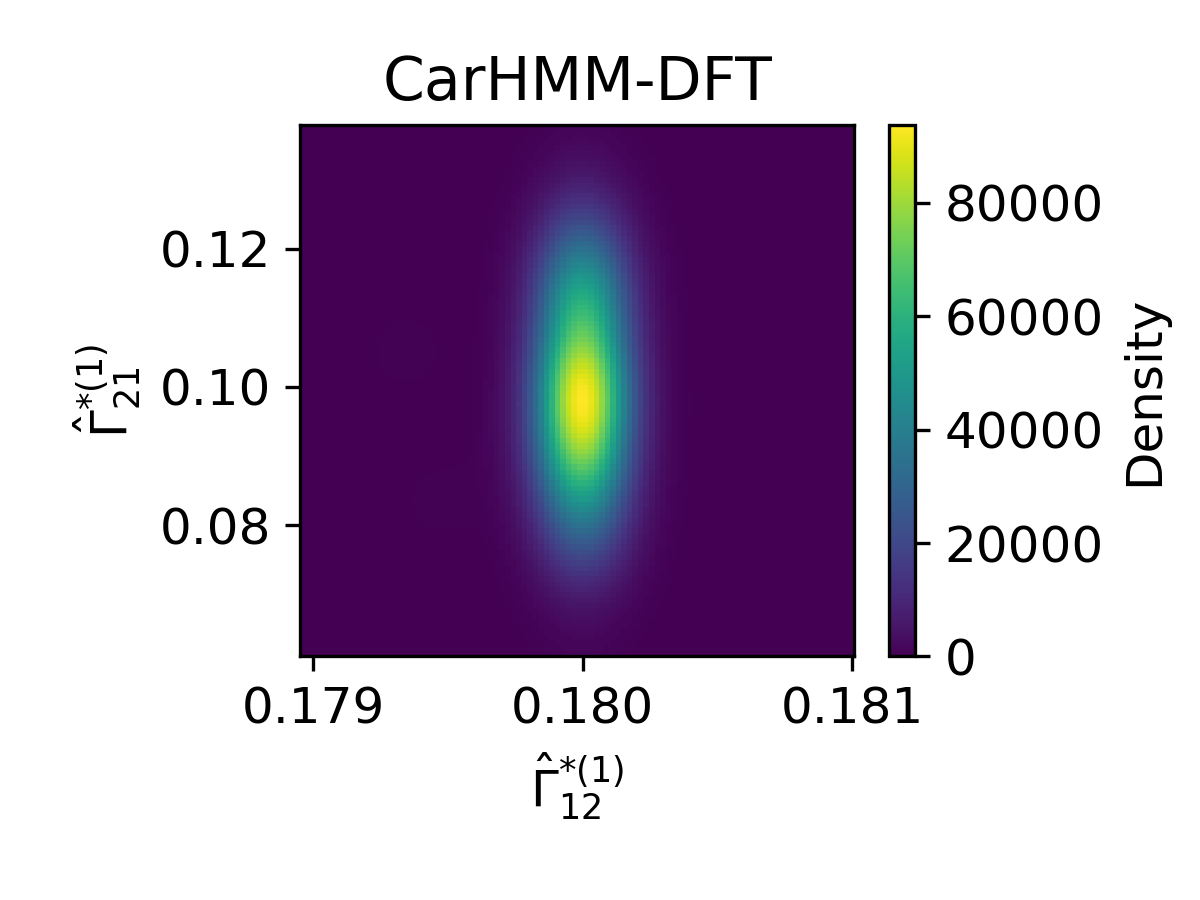
\includegraphics[width=5in]{../Plots/hmm_FV_Gamma_density_0.png}
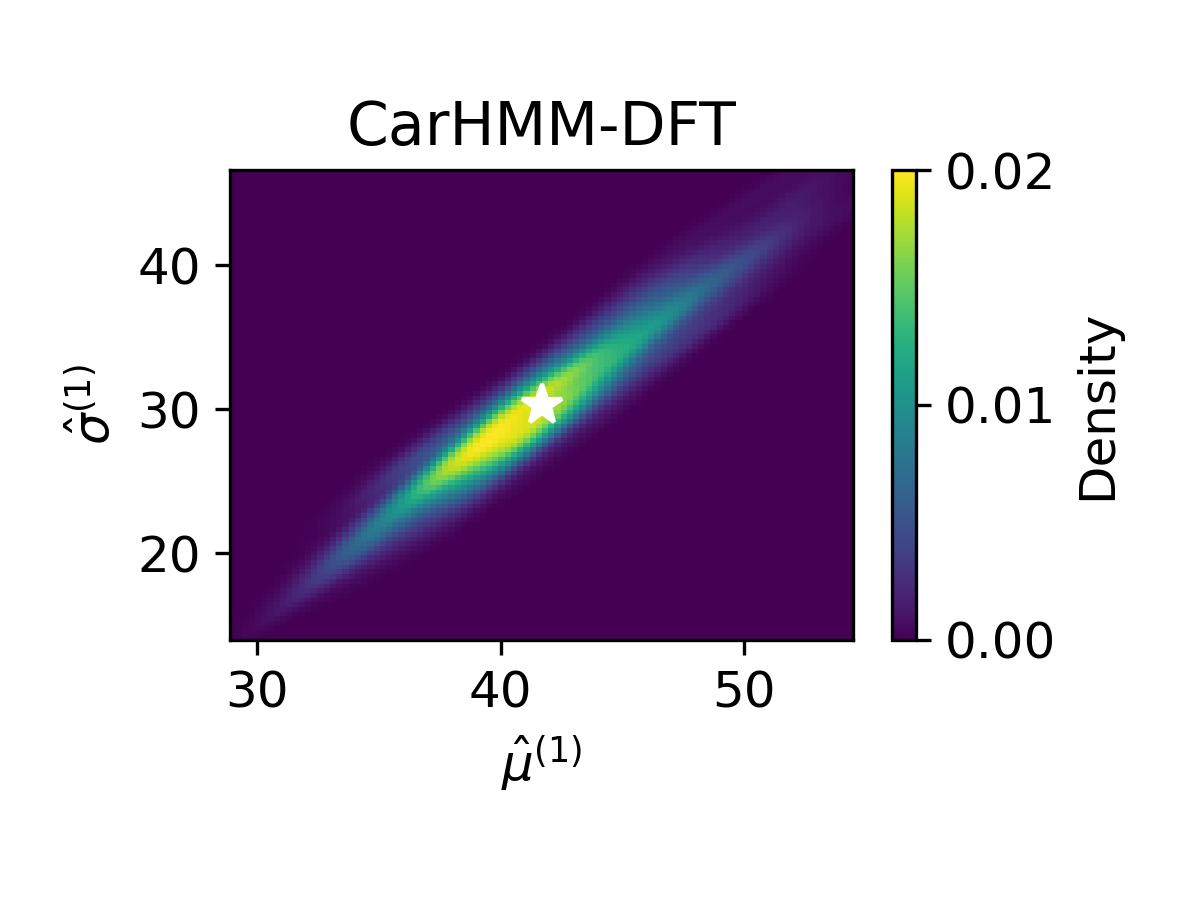
\includegraphics[width=5in]{../Plots/hmm_FV_MLE_density_dive_duration_-1_0.png}
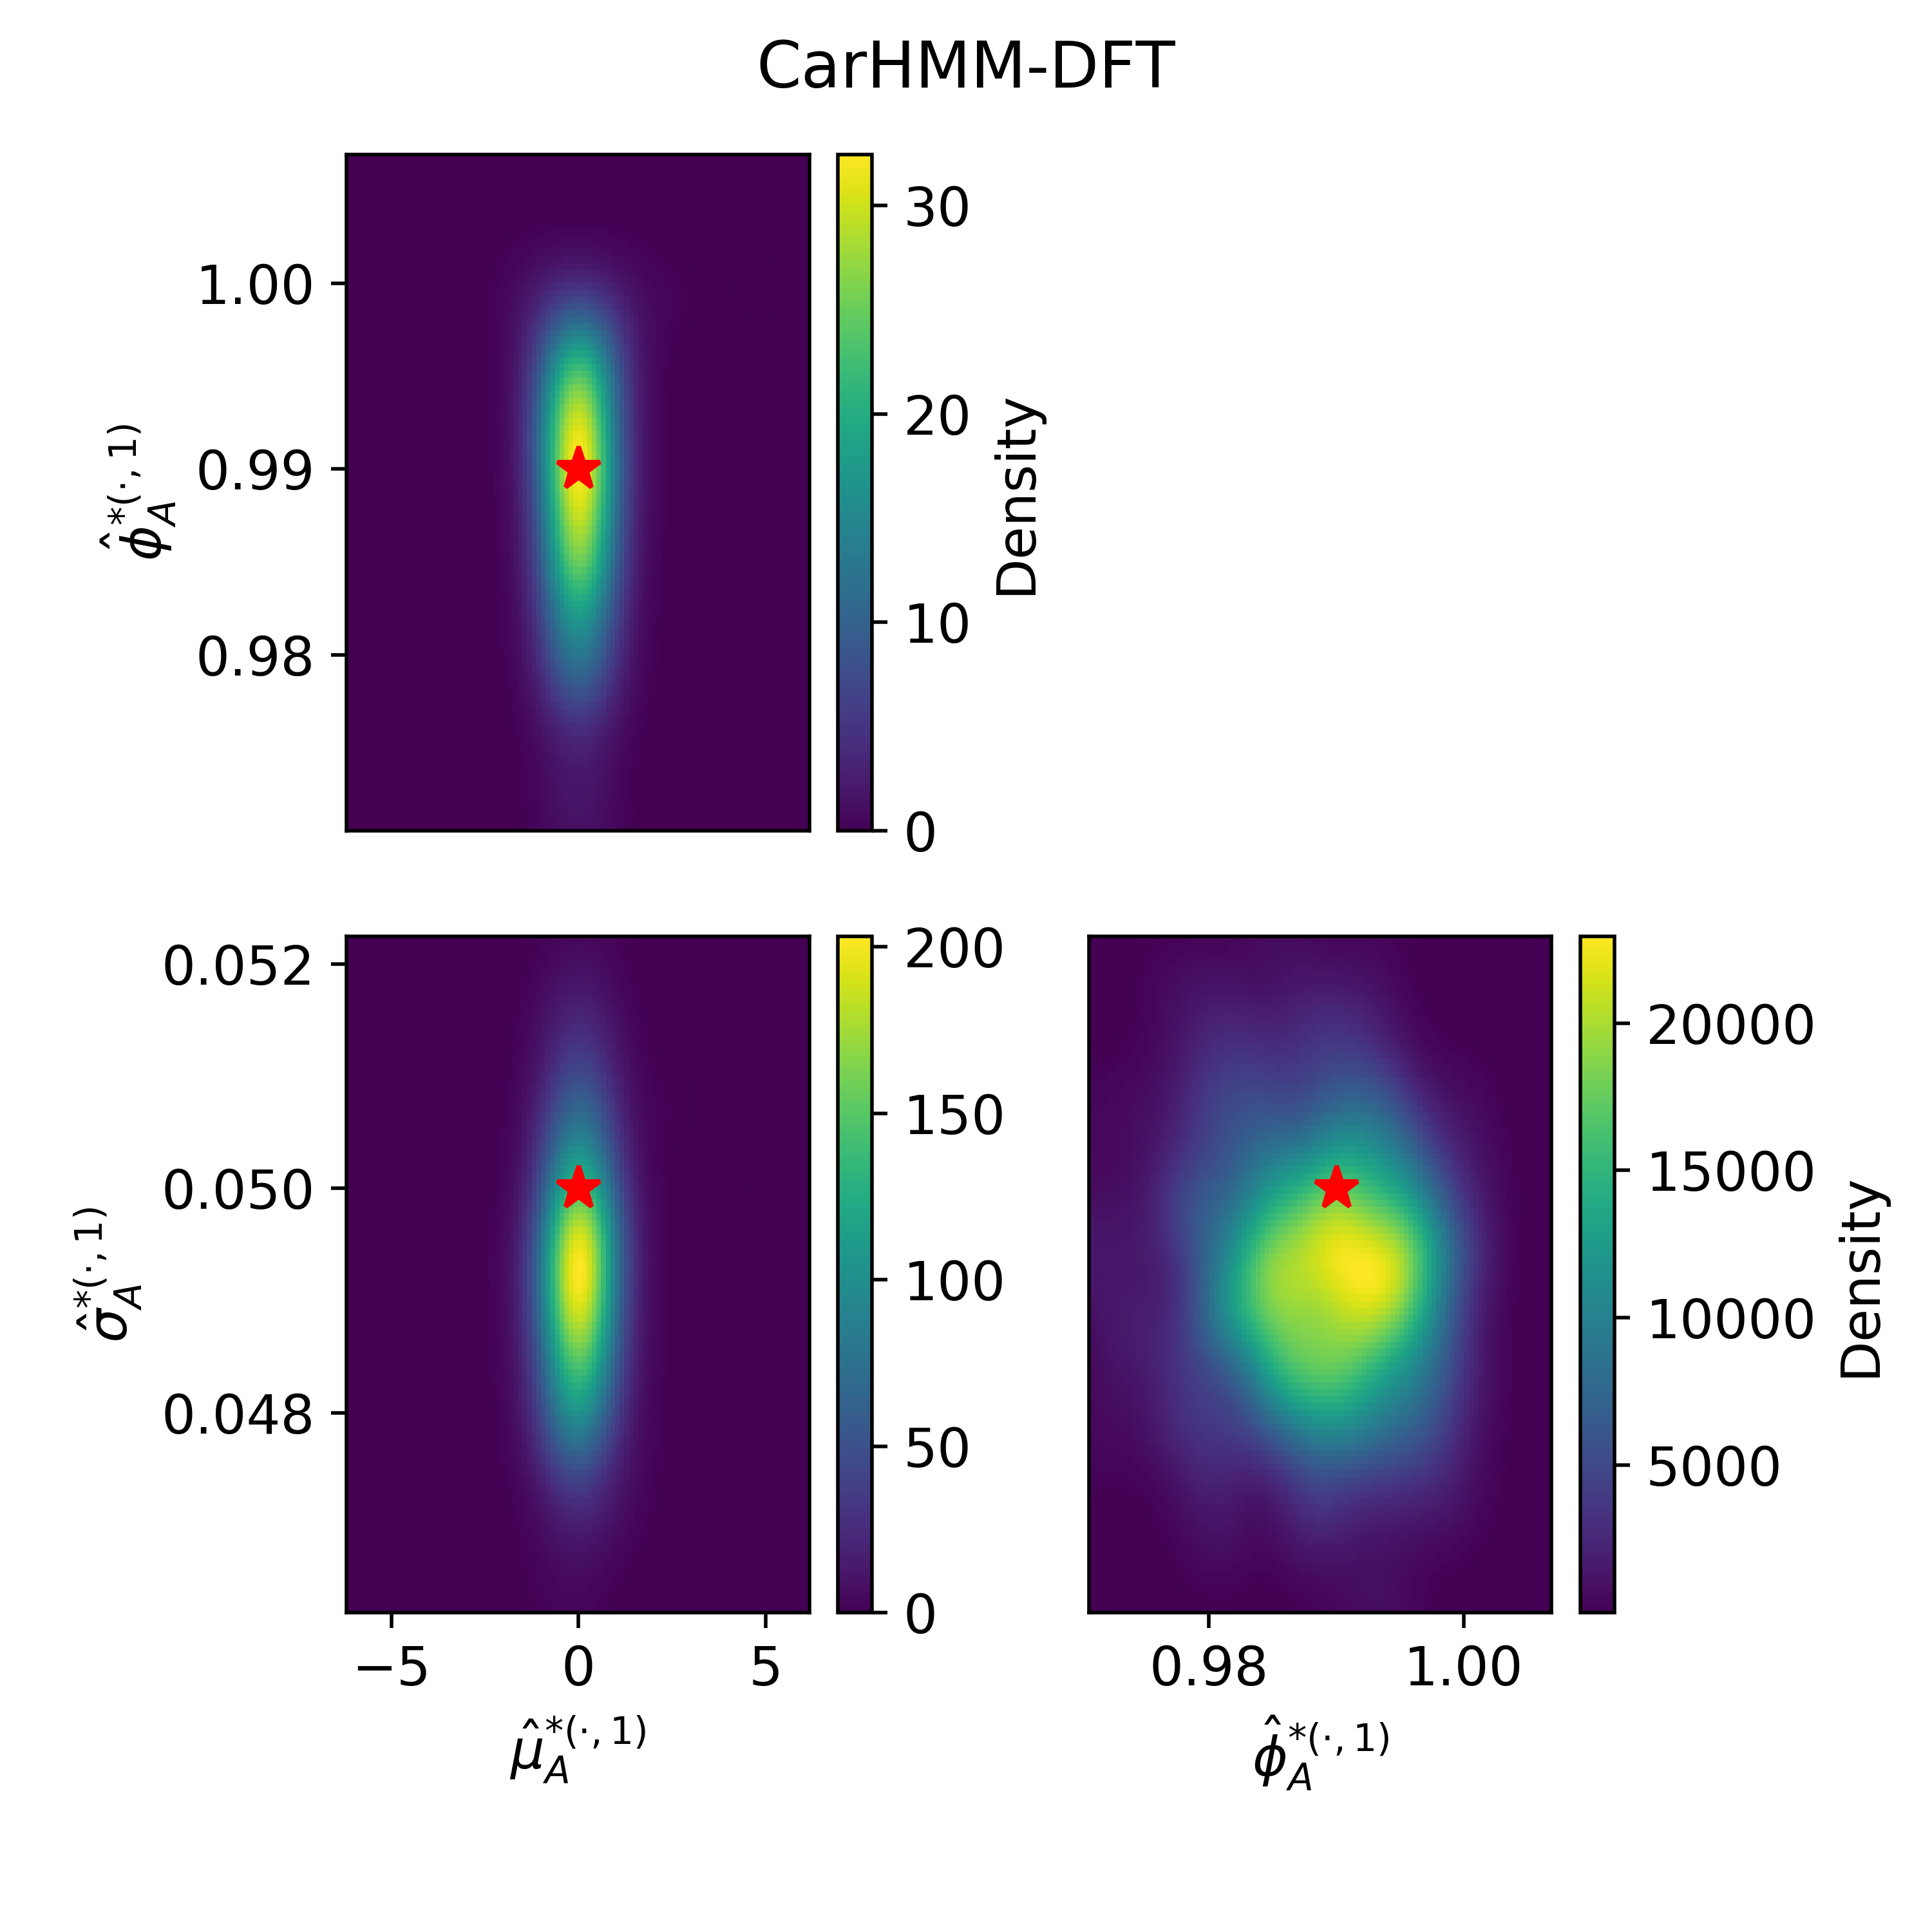
\includegraphics[height=4in]{../Plots/hmm_FV_MLE_density_A_0_0.png}
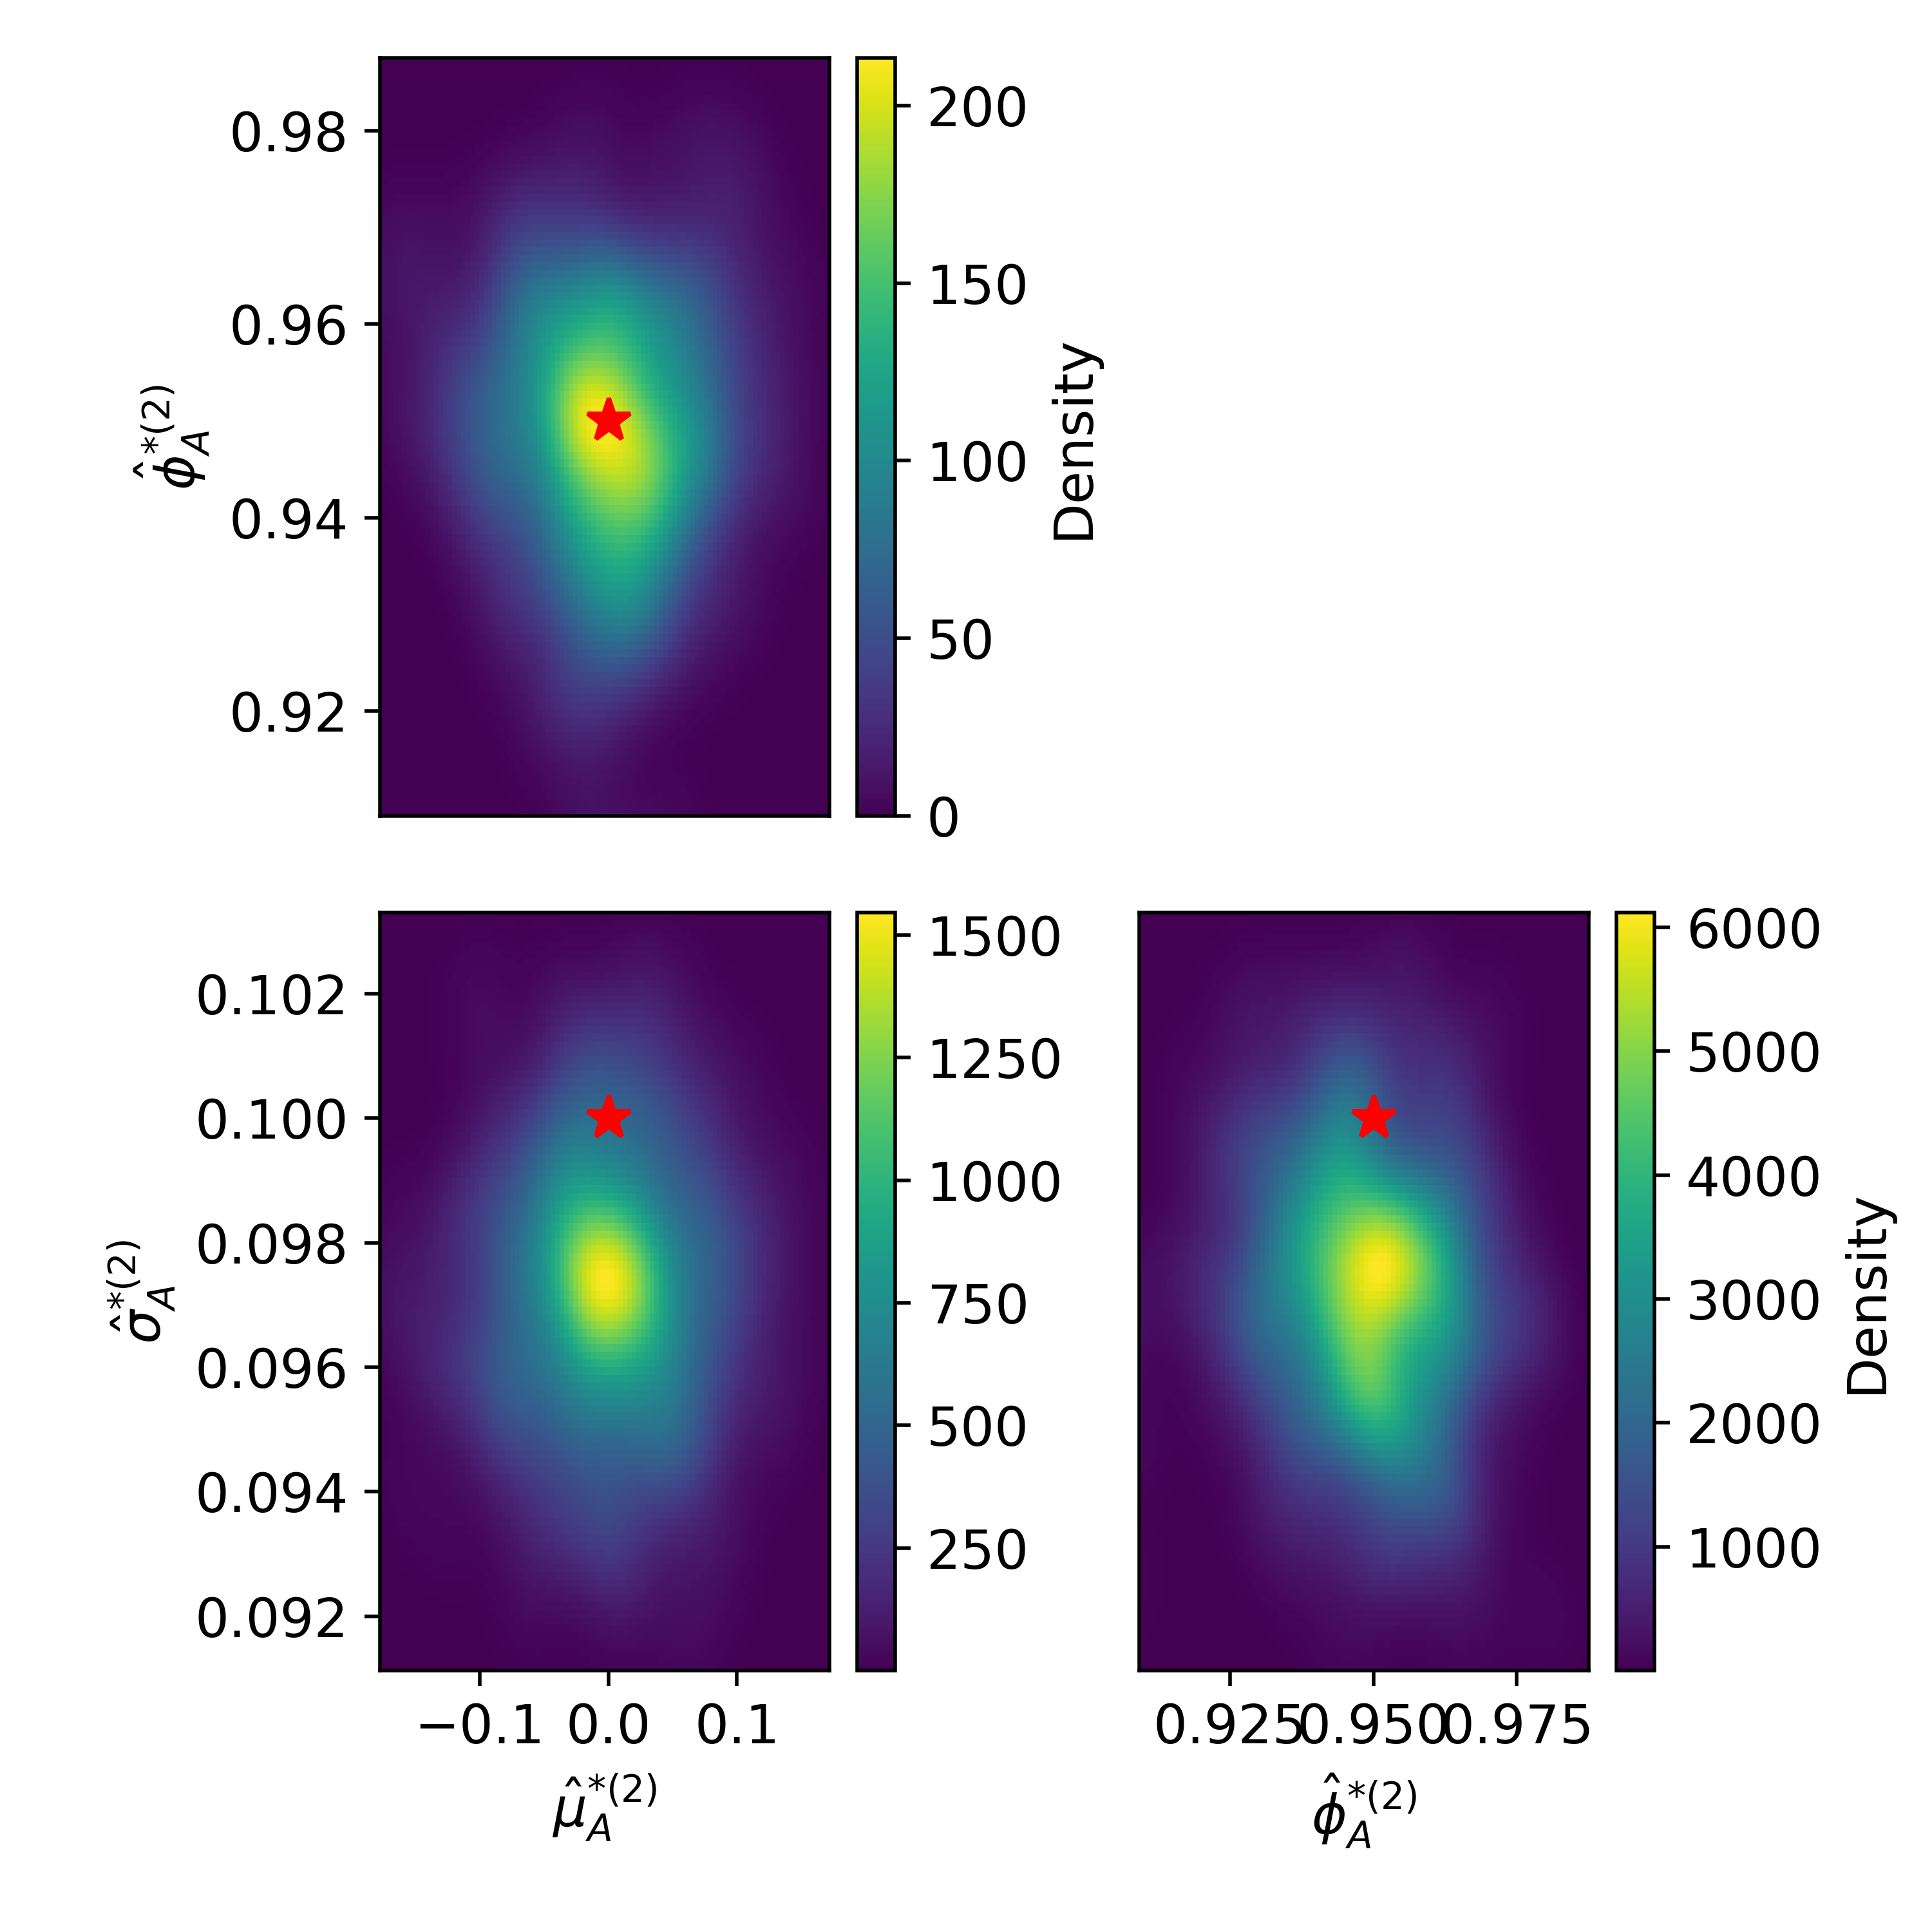
\includegraphics[height=4in]{../Plots/hmm_FV_MLE_density_A_0_1.png}
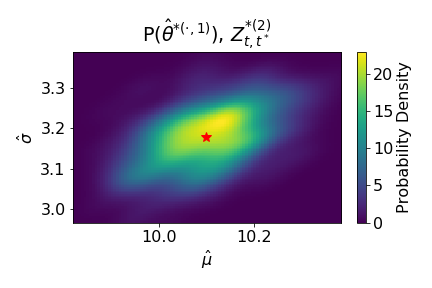
\includegraphics[width=2in]{../Plots/hmm_FV_MLE_density_FoVeDBA_0_0.png}
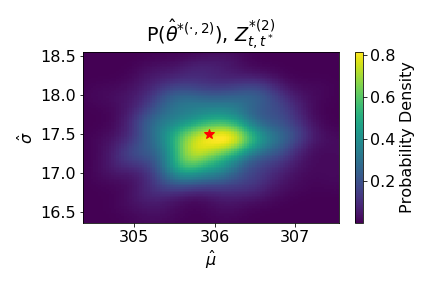
\includegraphics[width=2in]{../Plots/hmm_FV_MLE_density_FoVeDBA_0_1.png}

%%%%%%%%%%%%%%%%%%%%%%%%

\newpage
\subsubsection{\textbf{HHMM-DFT}}

The \textbf{HHMM-DFT} had no modelled auto-correlation, so the joint distribution of $\hat \theta^{*(\cdot,i^*)}$ is only two-dimensional ($\mu$ and $\sigma$) rather than three-dimensional.

\centering
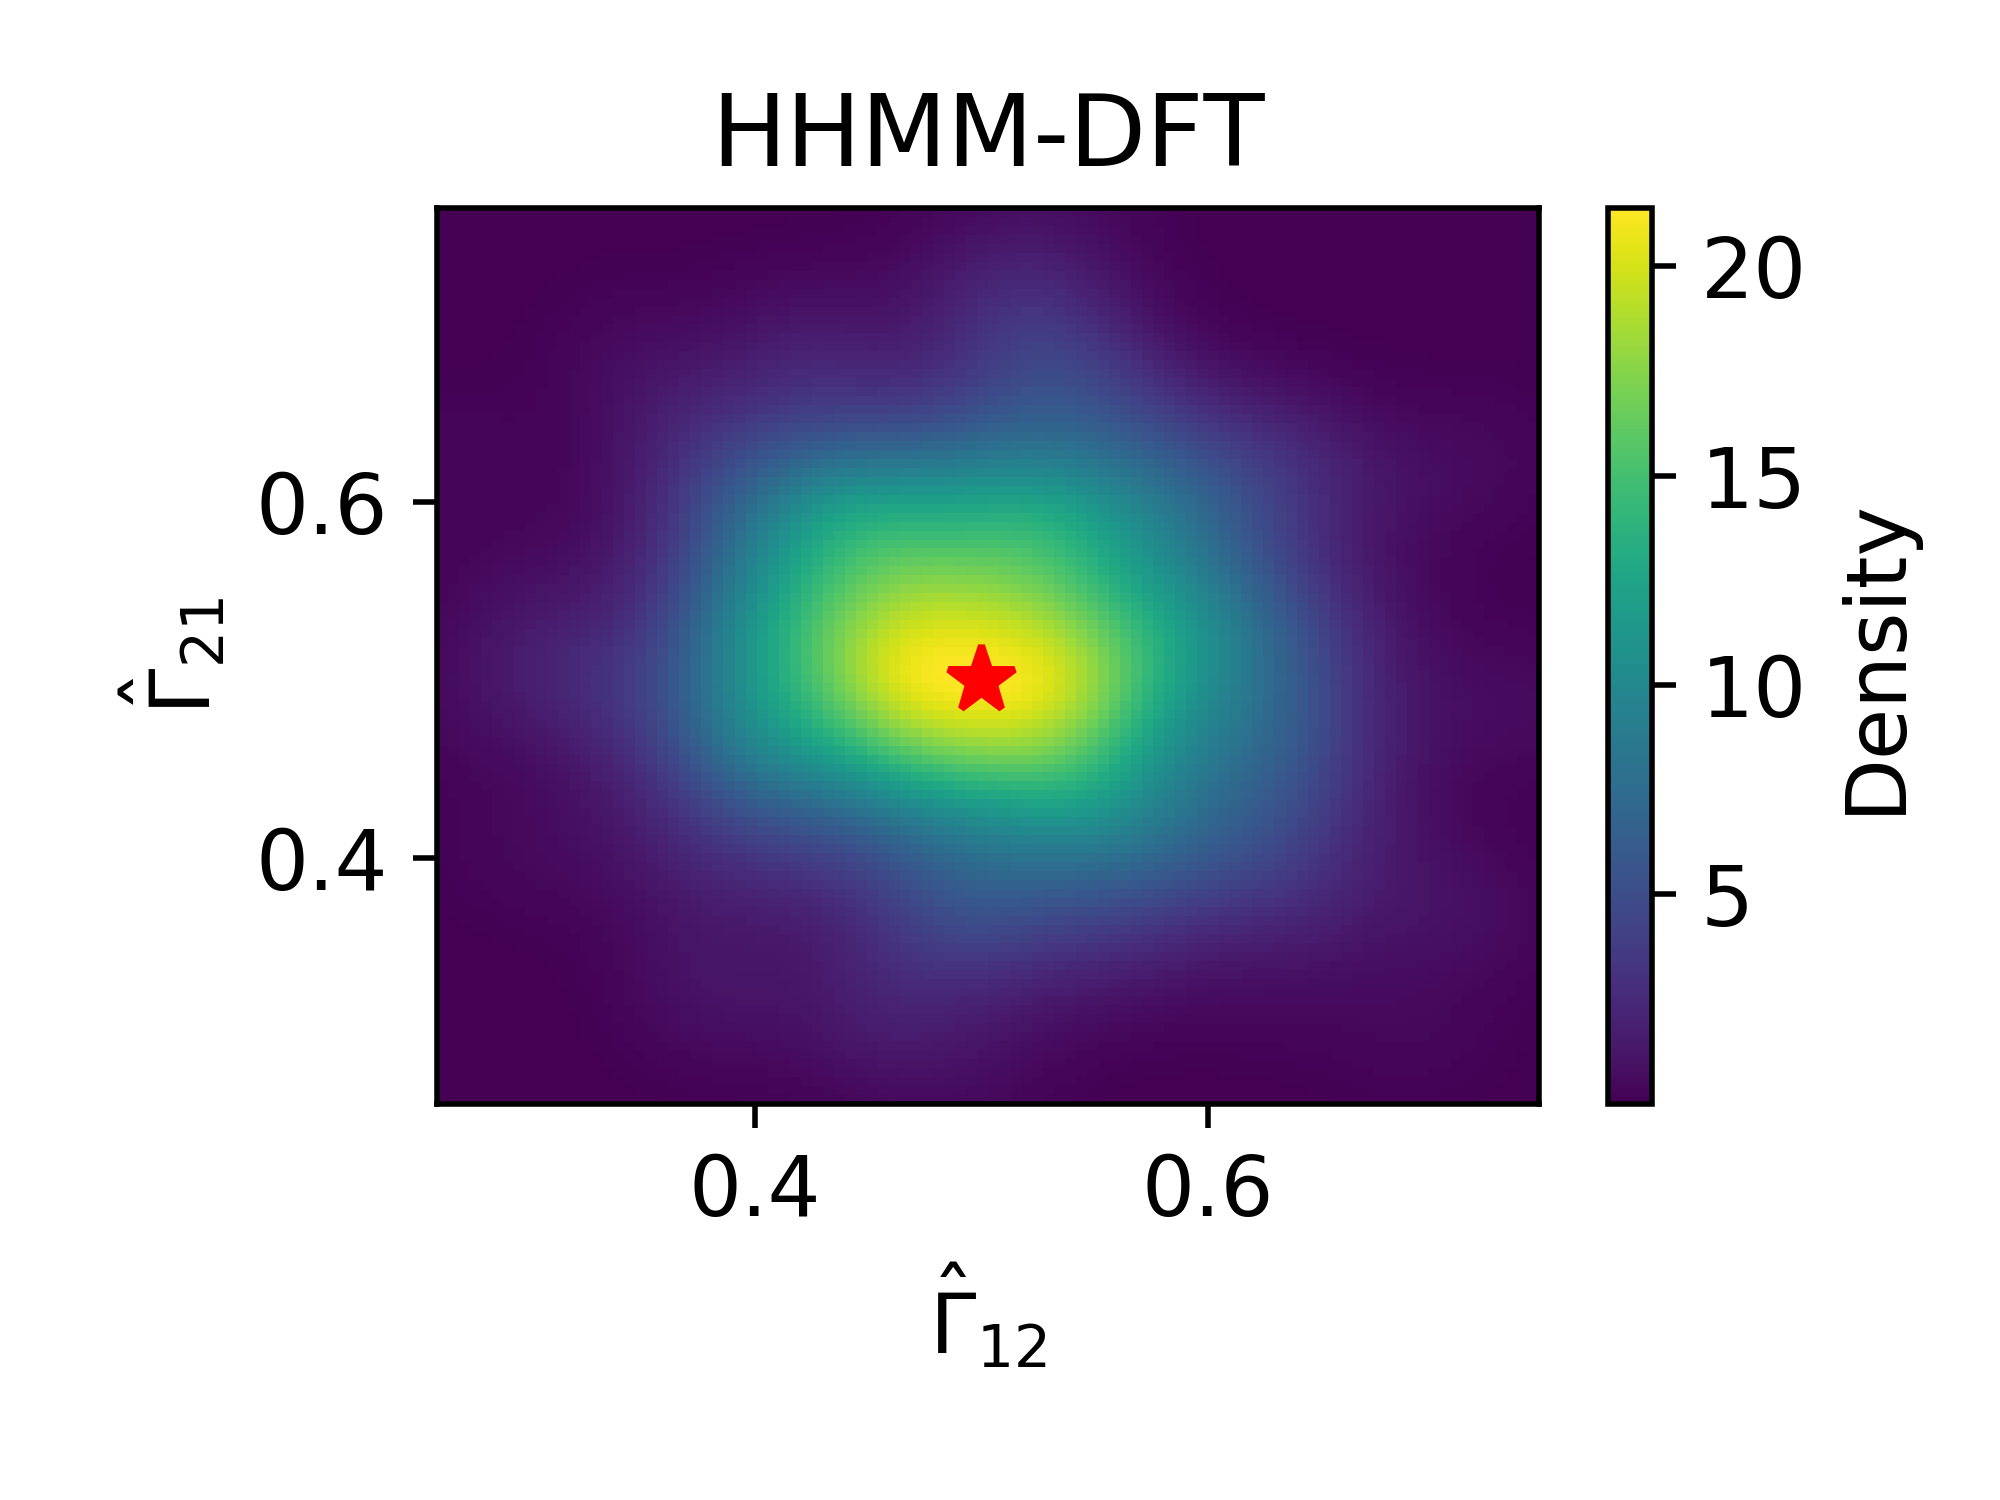
\includegraphics[width=5in]{../Plots/hhmm_FV_uncorr_Gamma_density_-1.png}
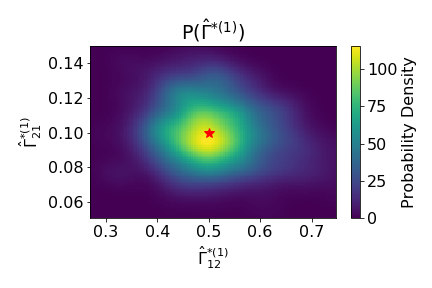
\includegraphics[width=2.25in]{../Plots/hhmm_FV_uncorr_Gamma_density_0.png}
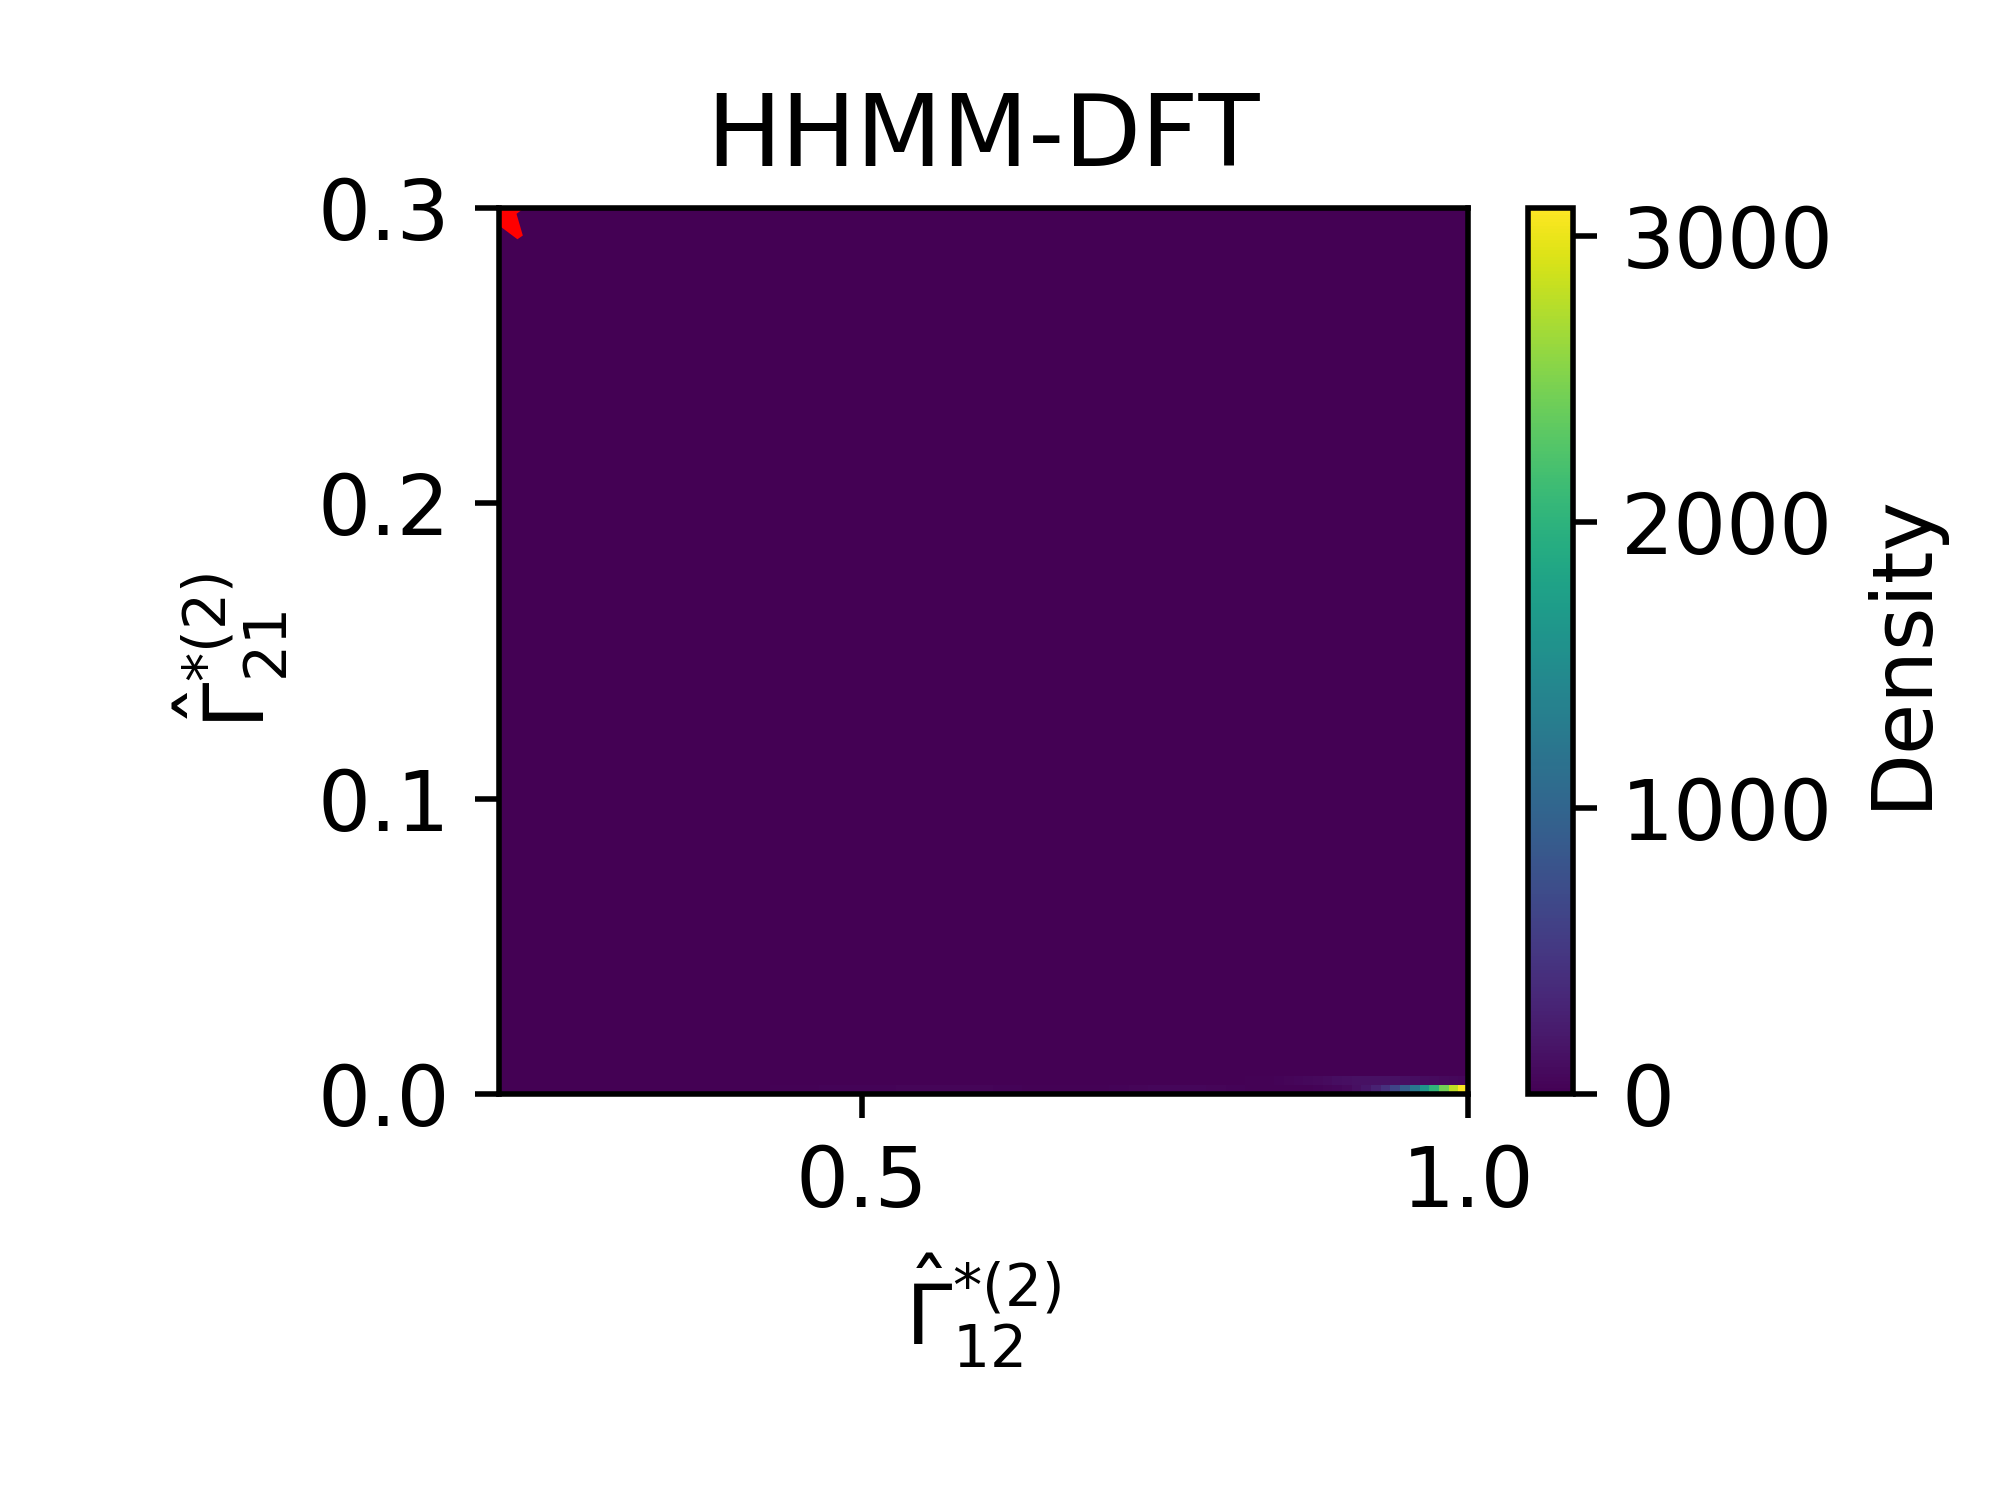
\includegraphics[width=2.25in]{../Plots/hhmm_FV_uncorr_Gamma_density_1.png}
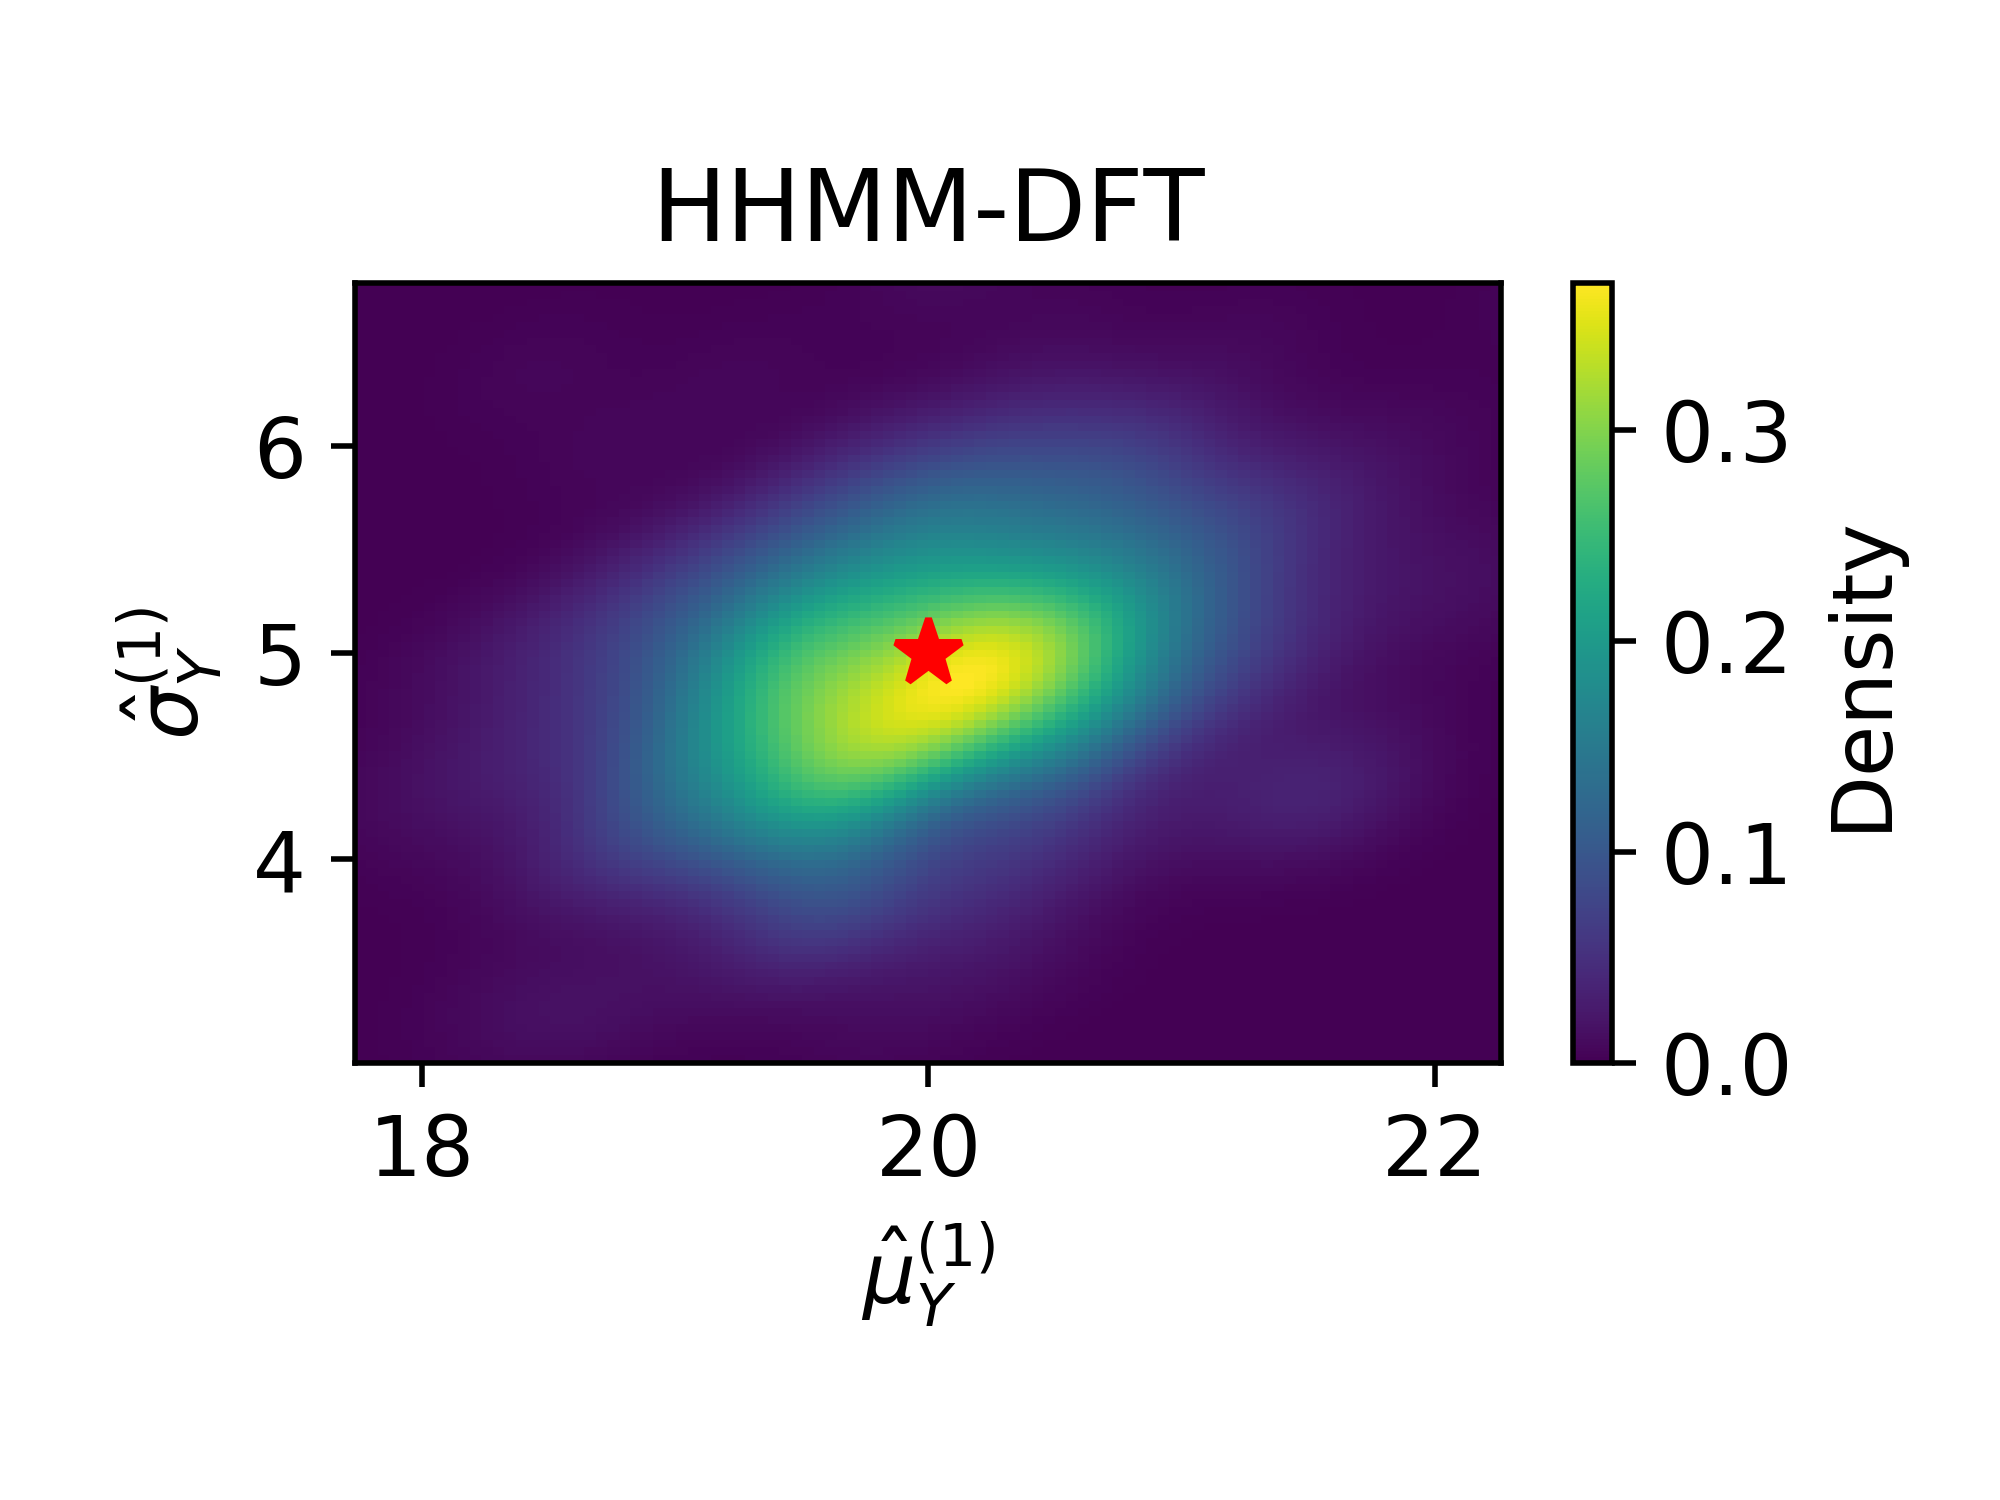
\includegraphics[width=2.25in]{../Plots/hhmm_FV_uncorr_MLE_density_dive_duration_-1_0.png}
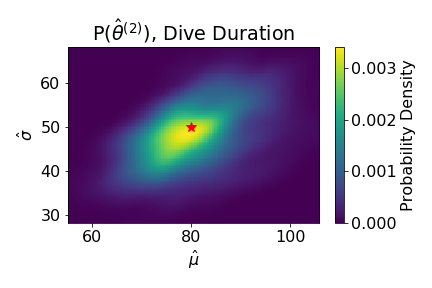
\includegraphics[width=2.25in]{../Plots/hhmm_FV_uncorr_MLE_density_dive_duration_-1_1.png}
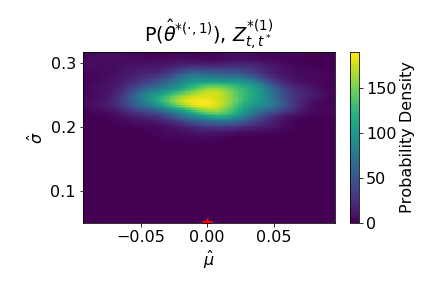
\includegraphics[width=2.25in]{../Plots/hhmm_FV_uncorr_MLE_density_A_0_0.png}
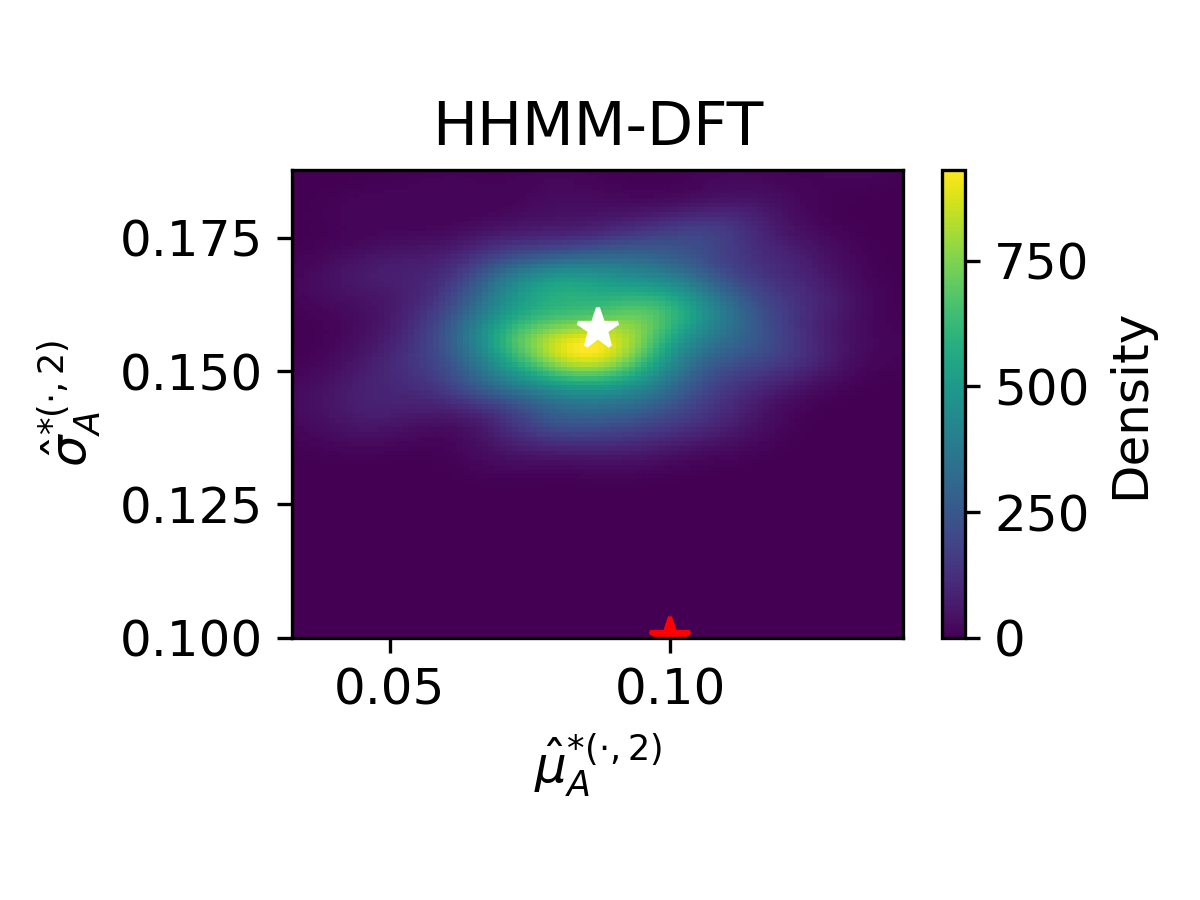
\includegraphics[width=2.25in]{../Plots/hhmm_FV_uncorr_MLE_density_A_0_1.png}
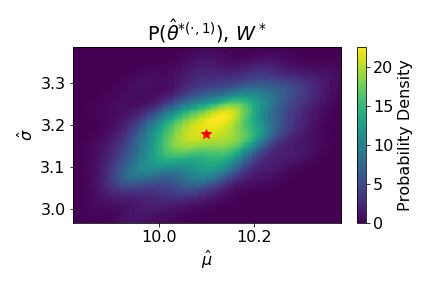
\includegraphics[width=2.25in]{../Plots/hhmm_FV_uncorr_MLE_density_FoVeDBA_0_0.png}
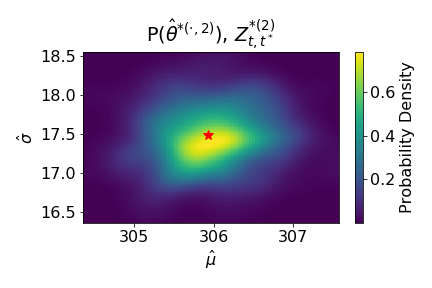
\includegraphics[width=2.25in]{../Plots/hhmm_FV_uncorr_MLE_density_FoVeDBA_0_1.png}

%%%%%%%%%%%%%%%%%%%%%%%%%%%%%%%%%

\newpage
\subsubsection{\textbf{CarHHMM}}

The \textbf{CarHHMM} lacks $Z^{*(2)}$ as an observation, so there is not distribution for $\hat Z^{*(2)}$ in the plots shown below.

\centering
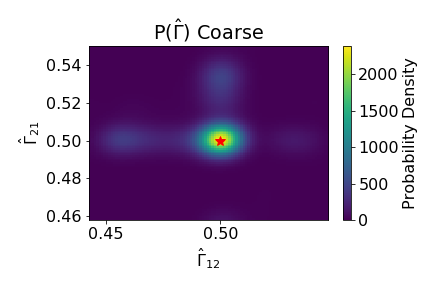
\includegraphics[width=5in]{../Plots/hhmm_V_Gamma_density_-1.png}
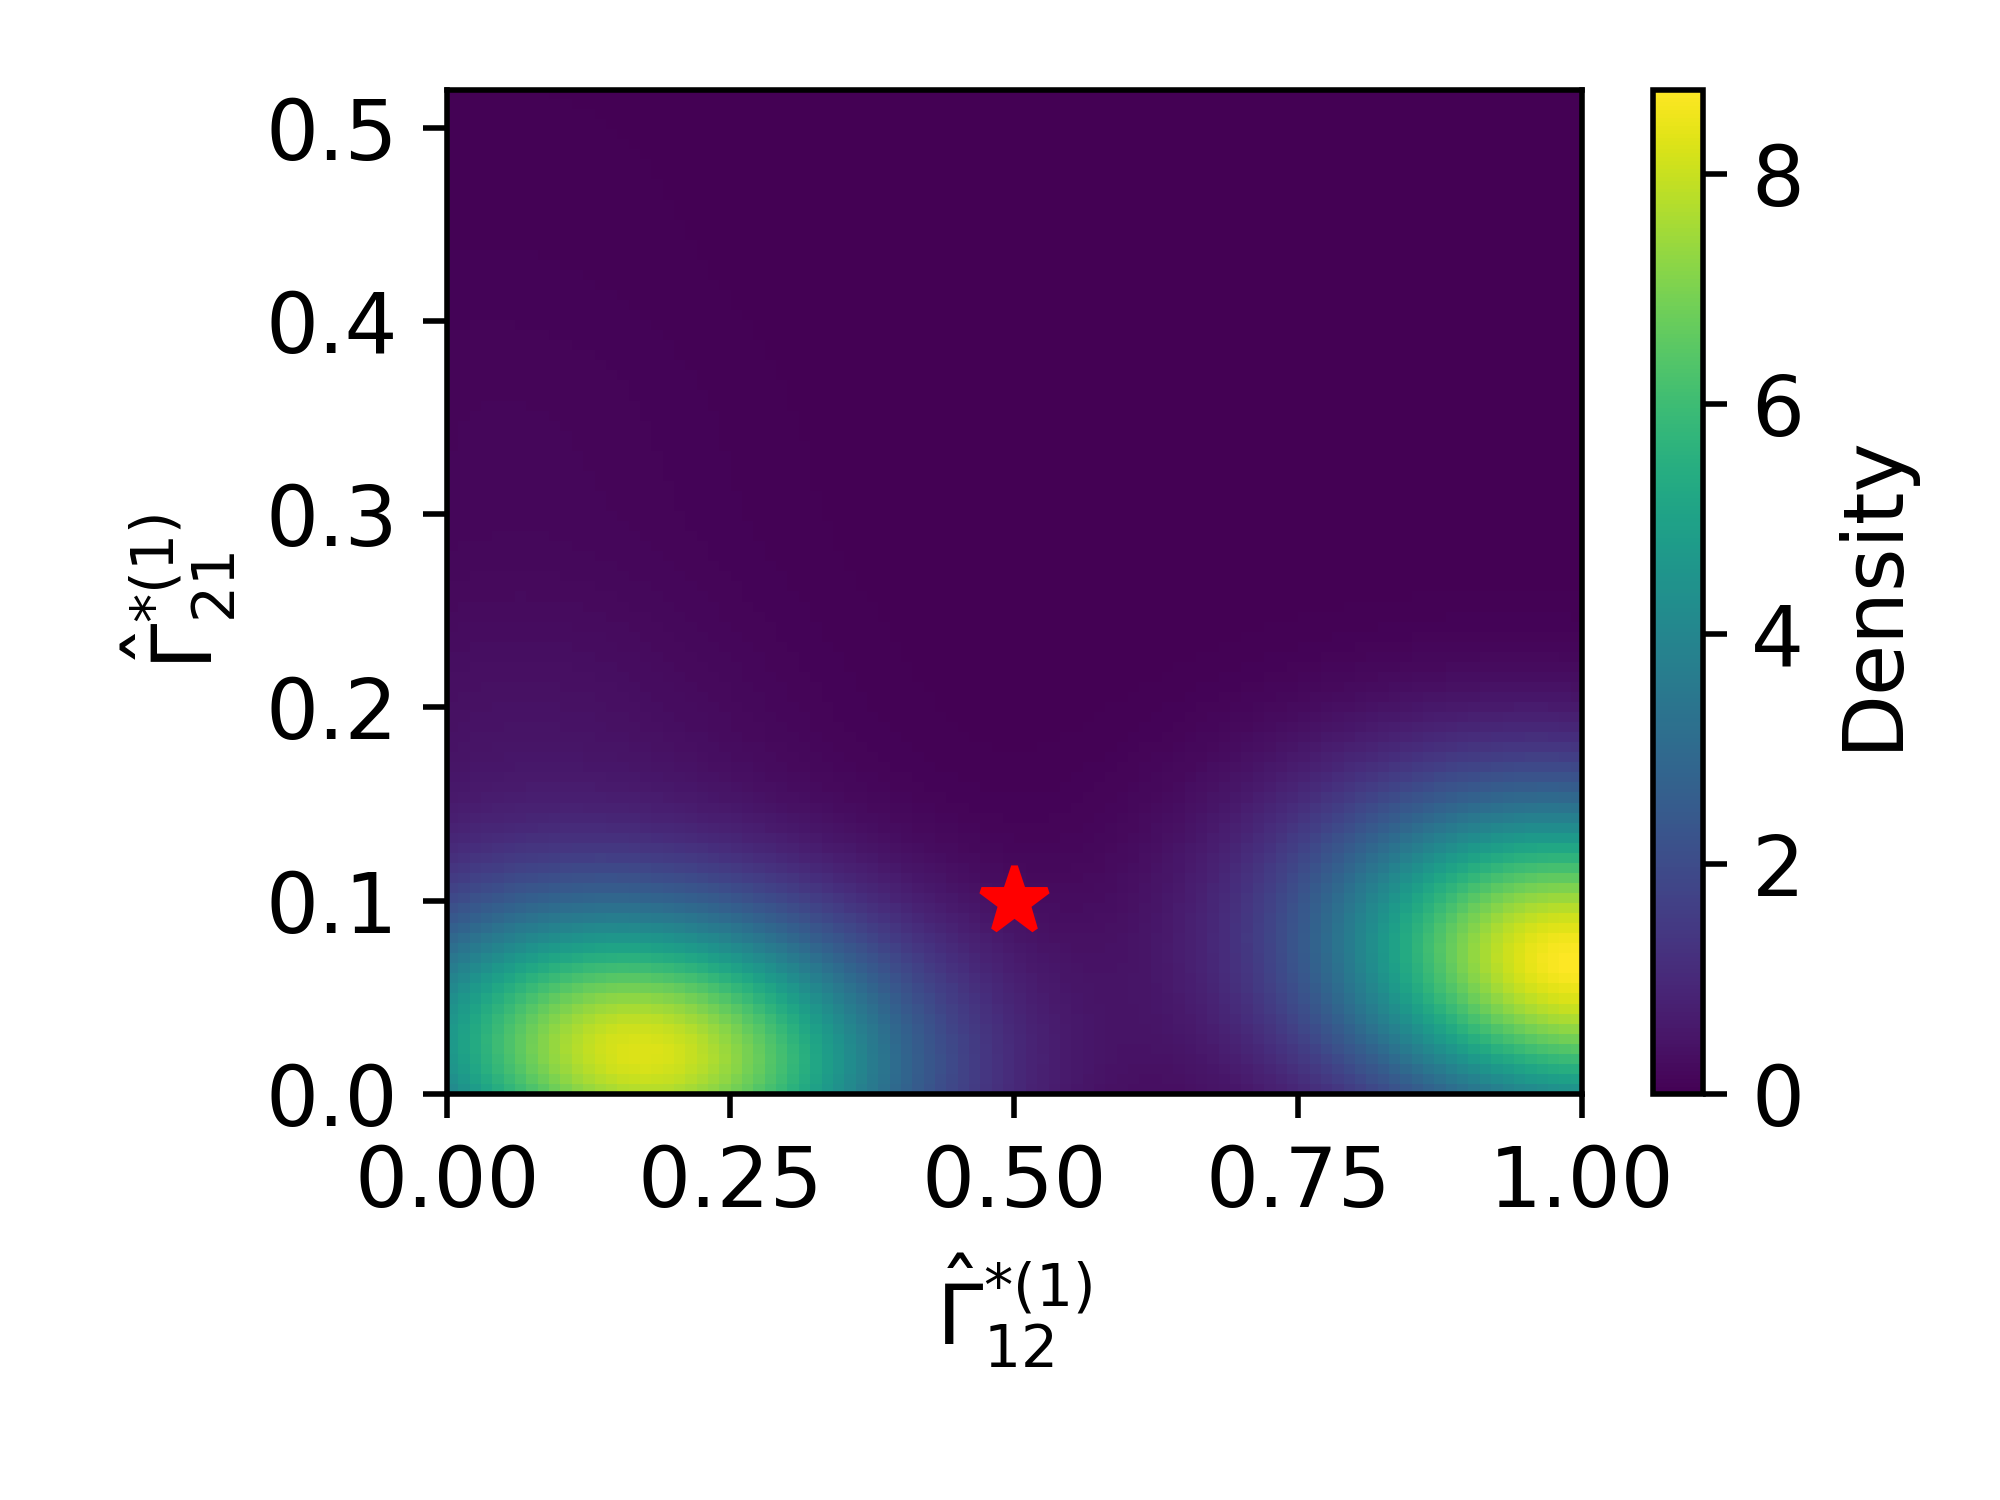
\includegraphics[width=2.25in]{../Plots/hhmm_V_Gamma_density_0.png}
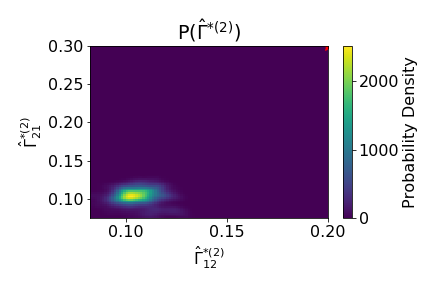
\includegraphics[width=2.25in]{../Plots/hhmm_V_Gamma_density_1.png}
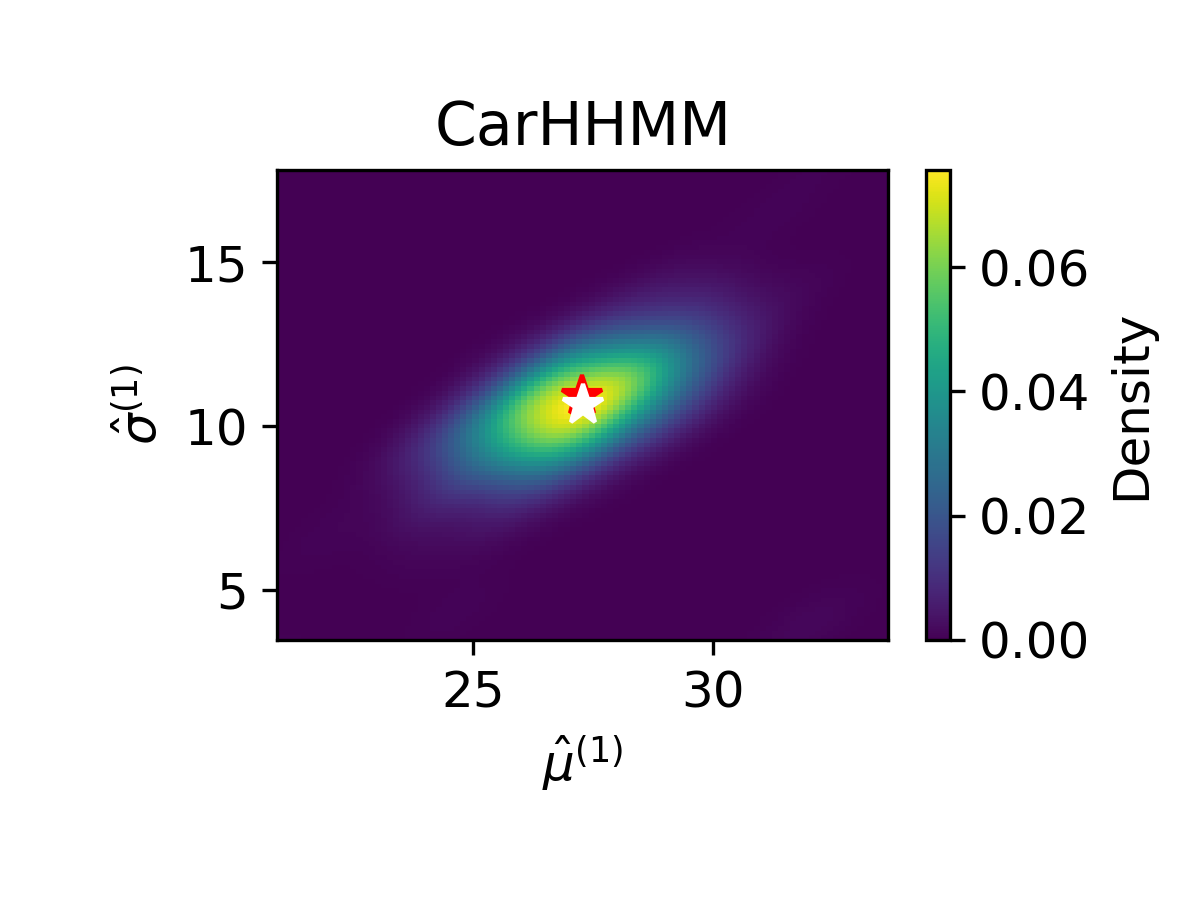
\includegraphics[width=2.25in]{../Plots/hhmm_V_MLE_density_dive_duration_-1_0.png}
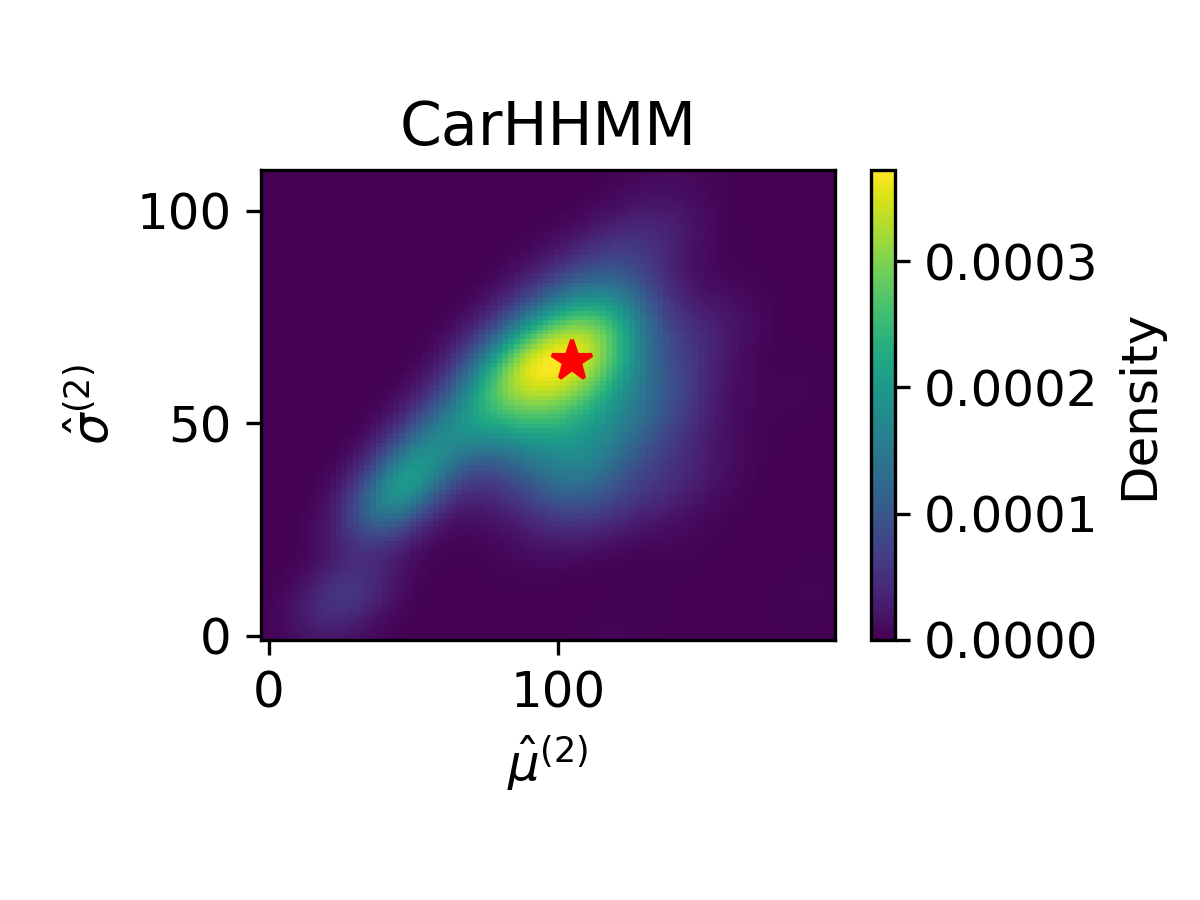
\includegraphics[width=2.25in]{../Plots/hhmm_V_MLE_density_dive_duration_-1_1.png}
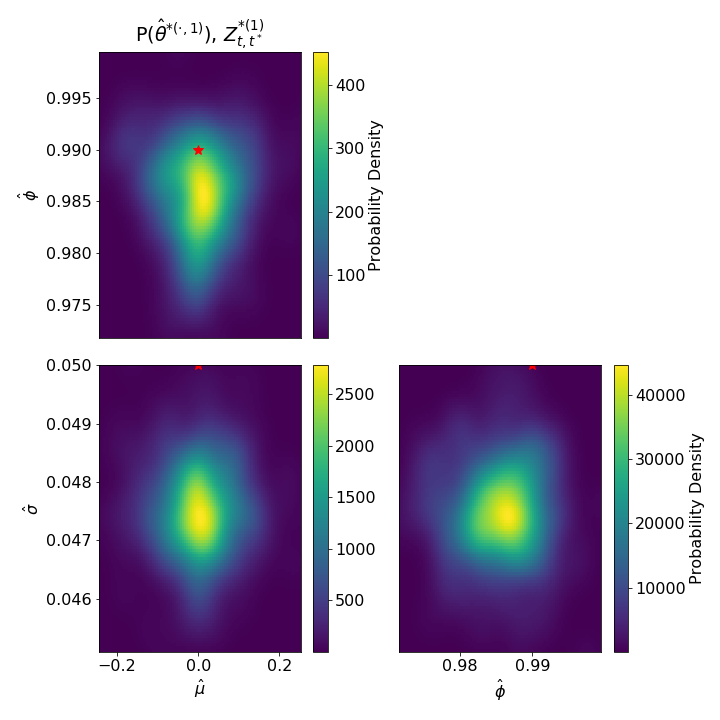
\includegraphics[height=4in]{../Plots/hhmm_V_MLE_density_A_0_0.png}
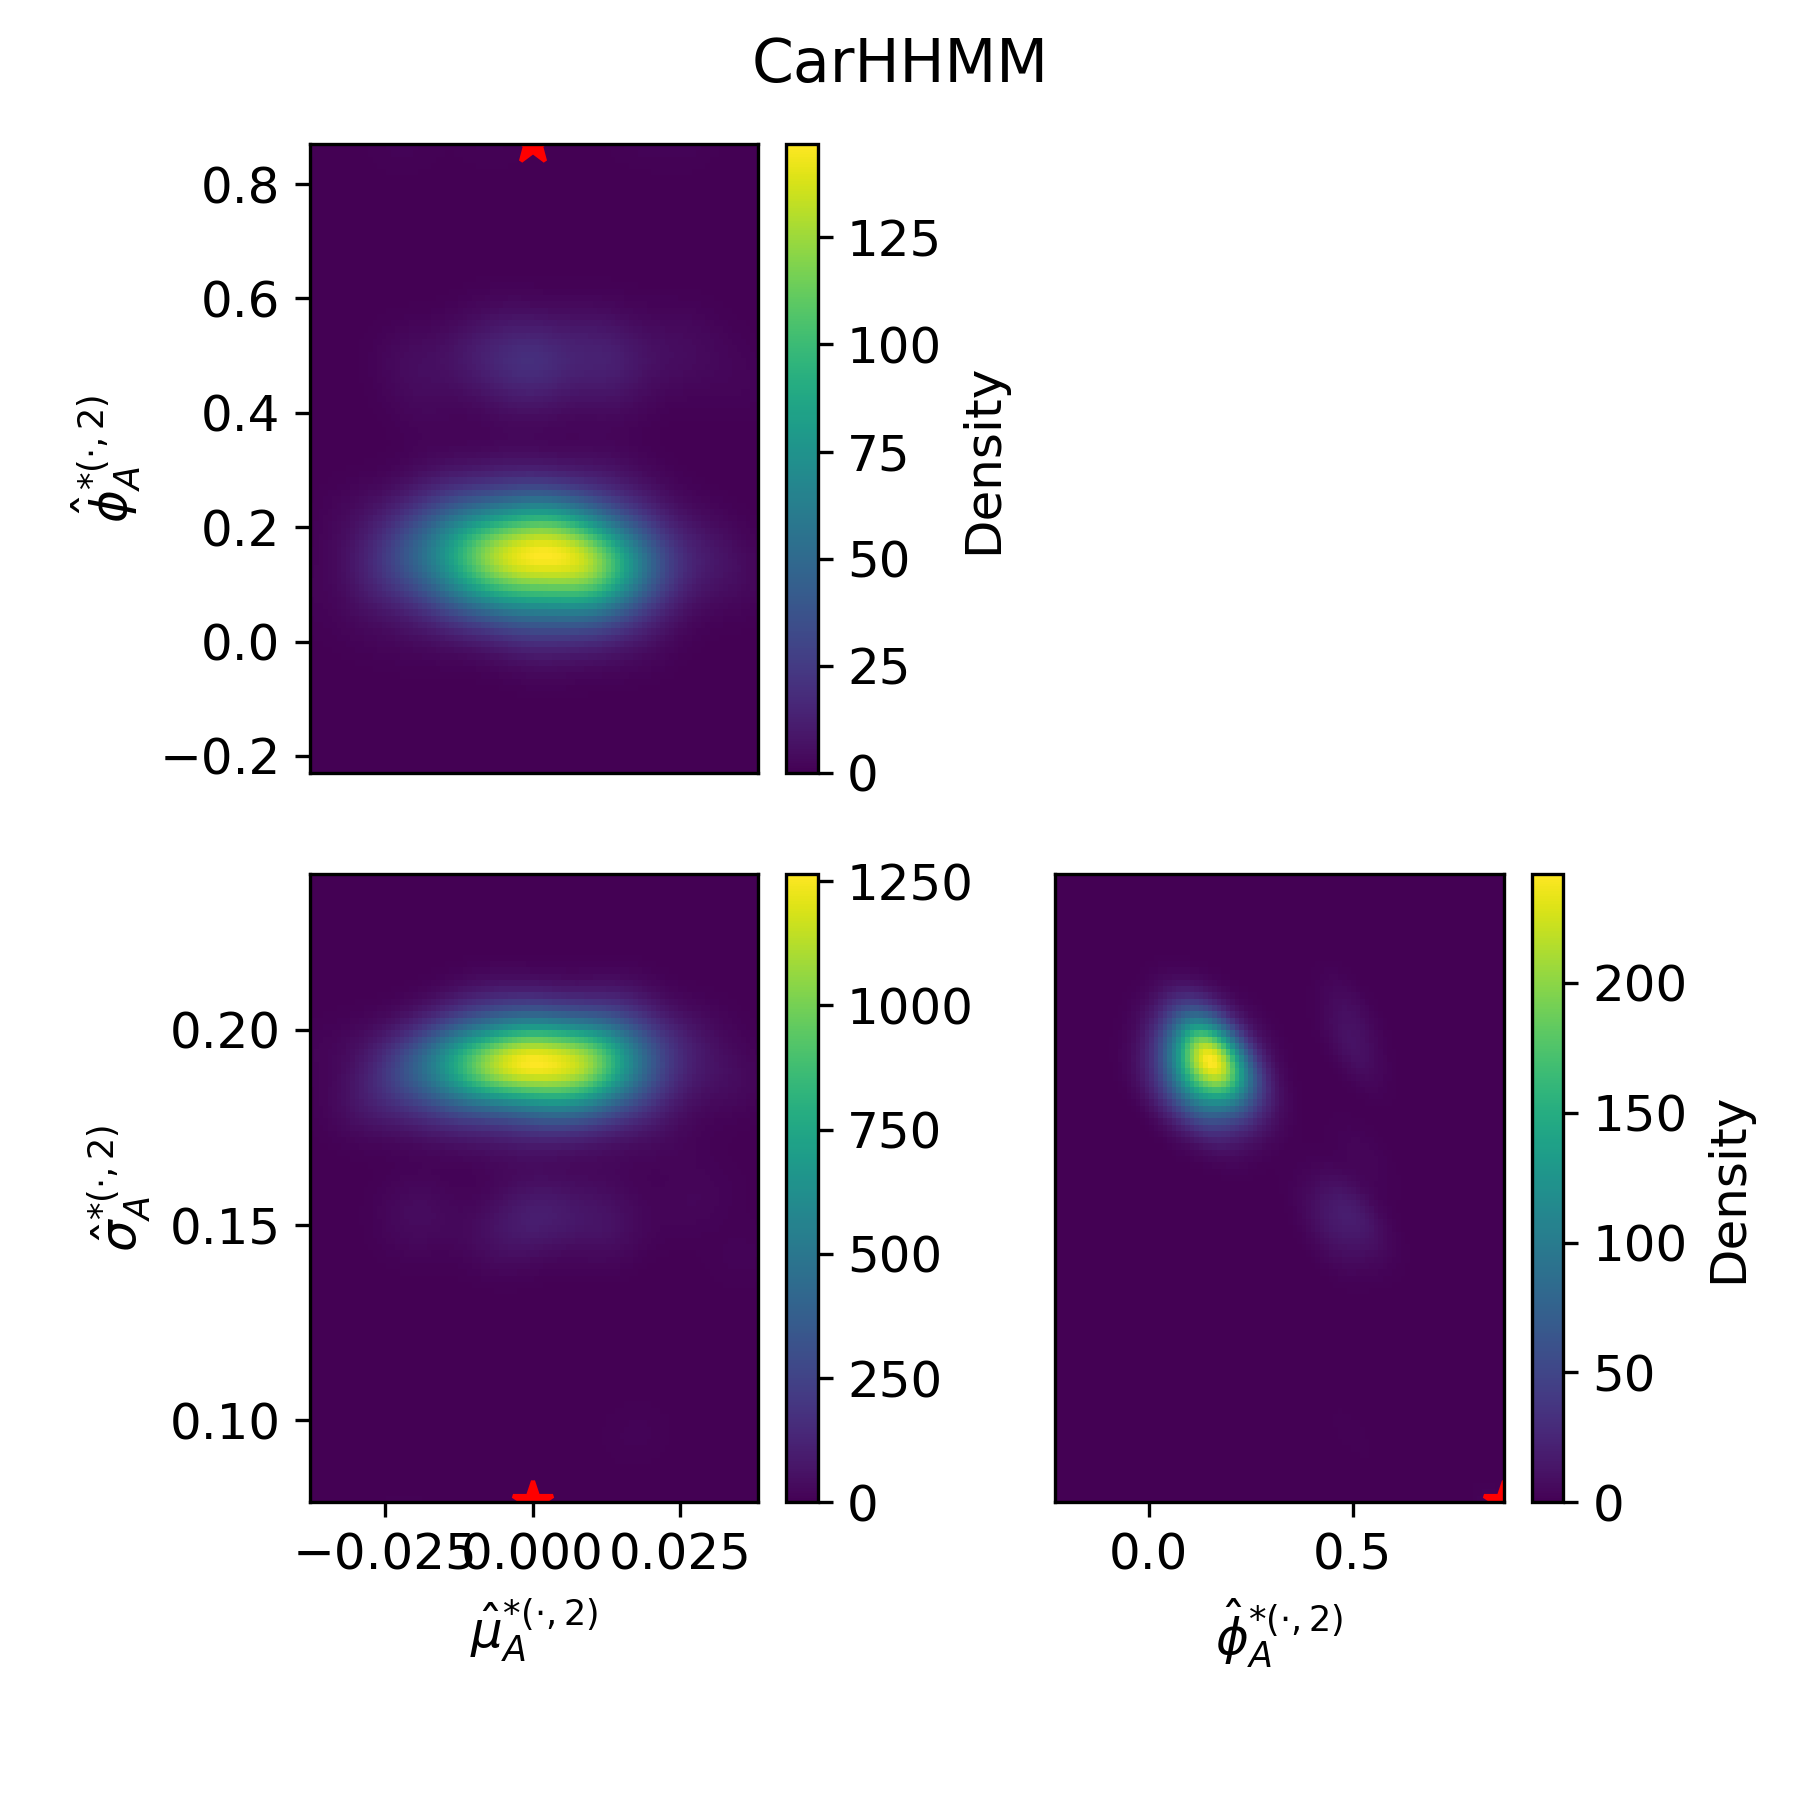
\includegraphics[height=4in]{../Plots/hhmm_V_MLE_density_A_0_1.png}

%%%%%%%%%%%%%%%%%%%%%%%%%%%%%%%%%

\newpage
\subsubsection{\textbf{CarHHMM-DFT}}

The \textbf{CarHHMM-DFT} is well-specified for the data from the simulation study. 

\centering
The \textbf{CarHHM-DFT}
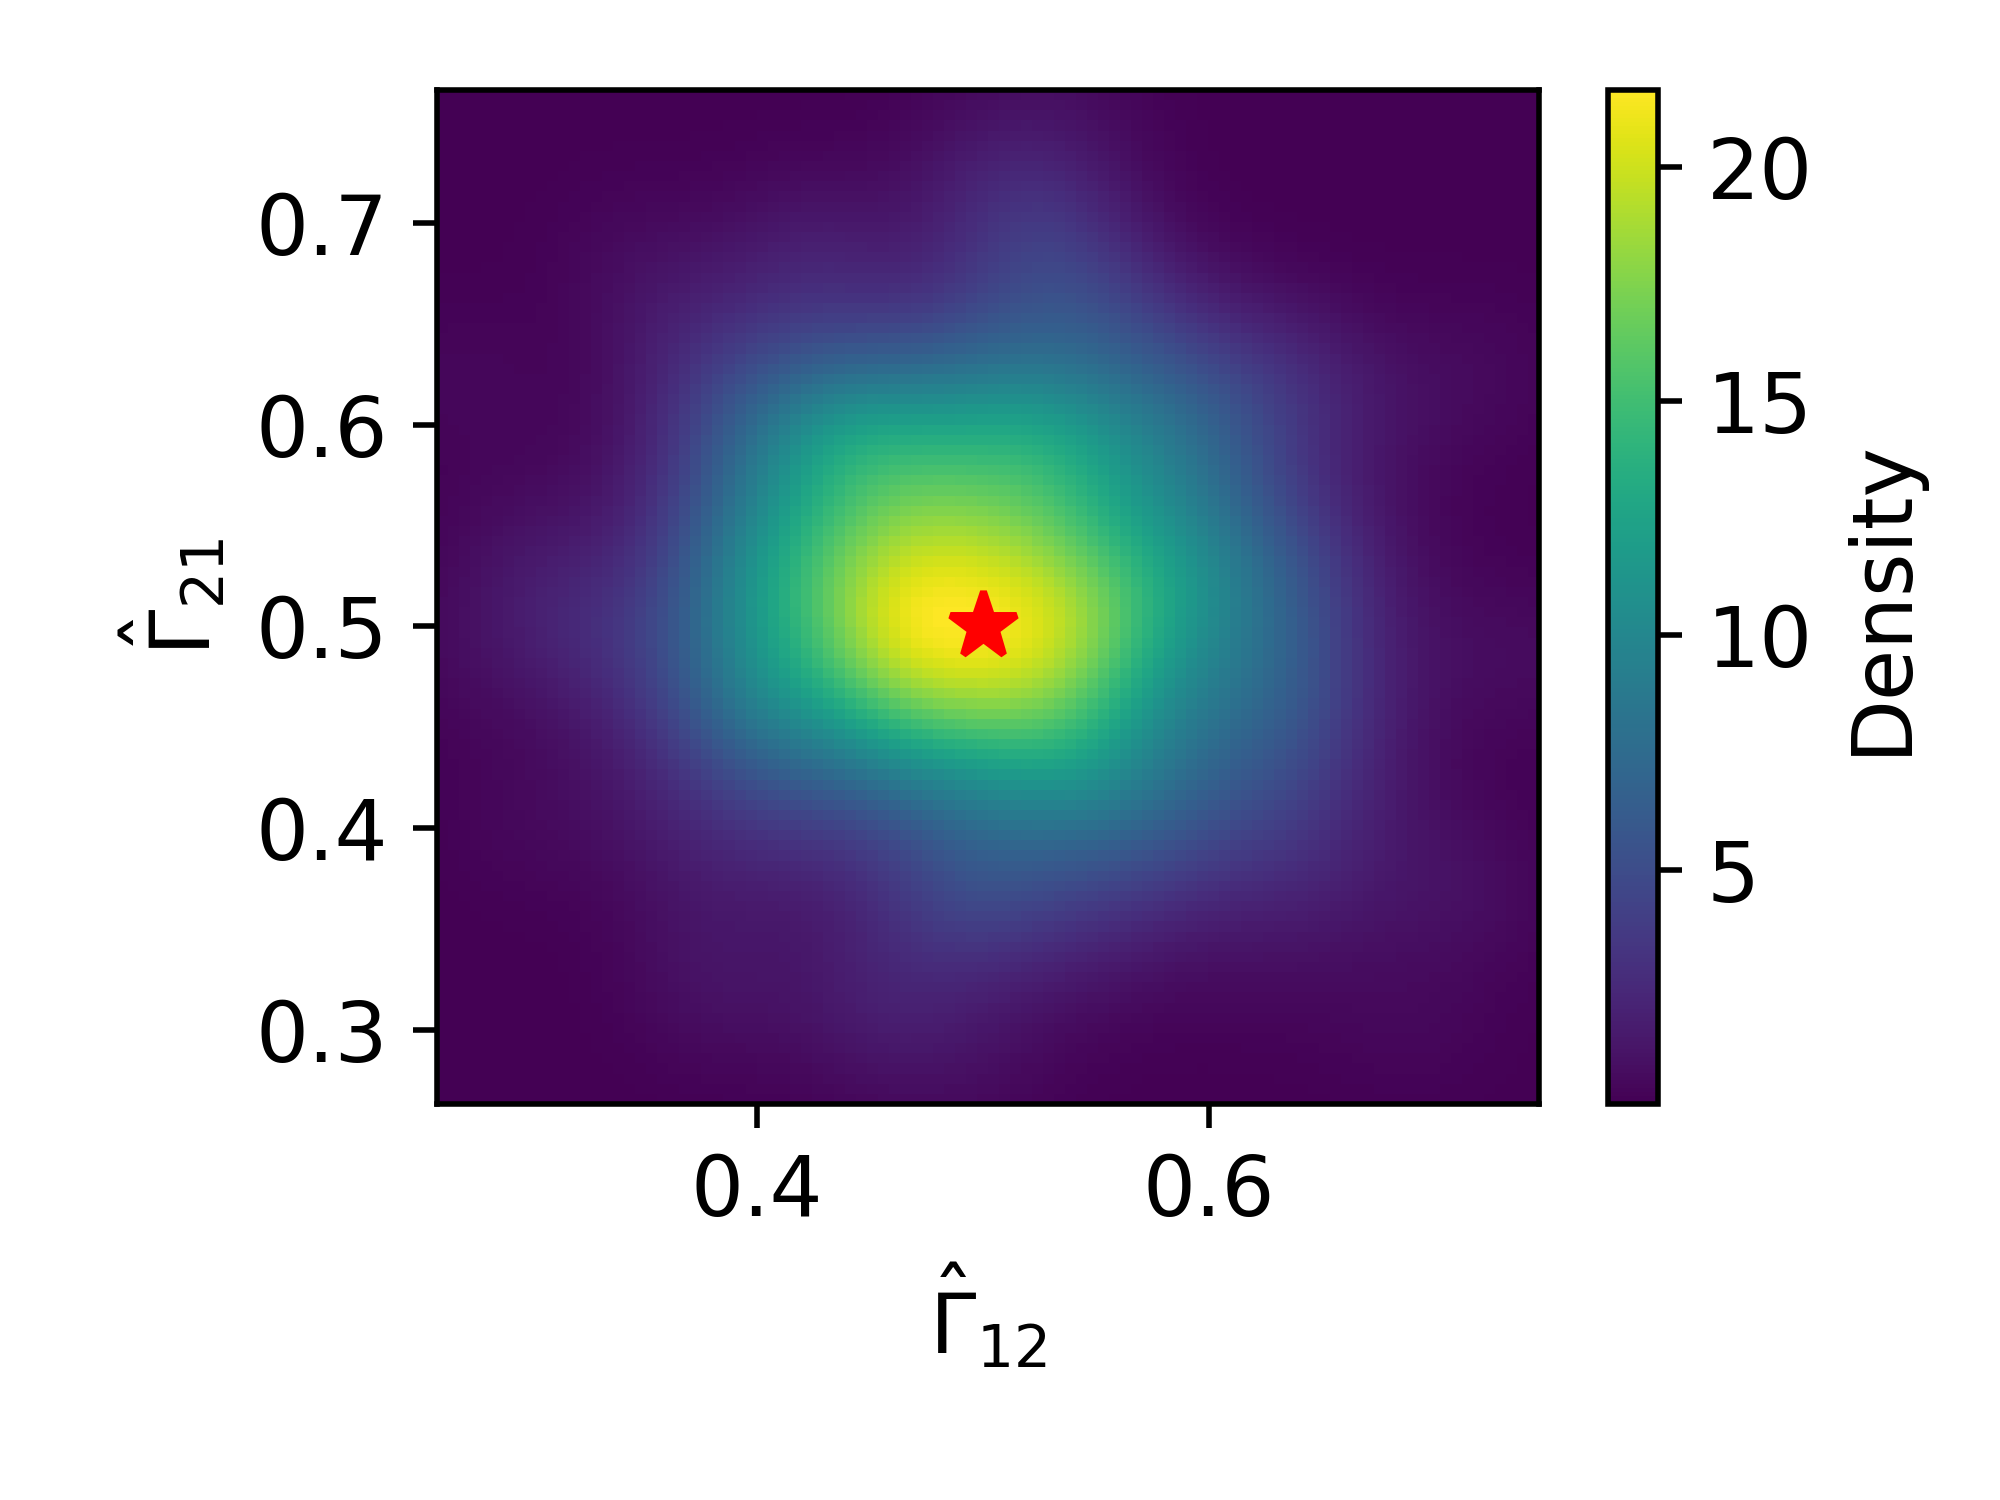
\includegraphics[width=5in]{../Plots/hhmm_FV_Gamma_density_-1.png}
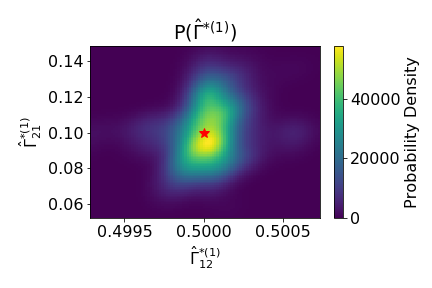
\includegraphics[width=2.25in]{../Plots/hhmm_FV_Gamma_density_0.png}
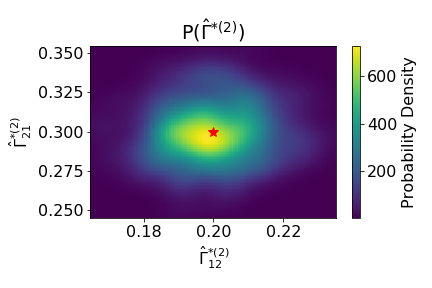
\includegraphics[width=2.25in]{../Plots/hhmm_FV_Gamma_density_1.png}
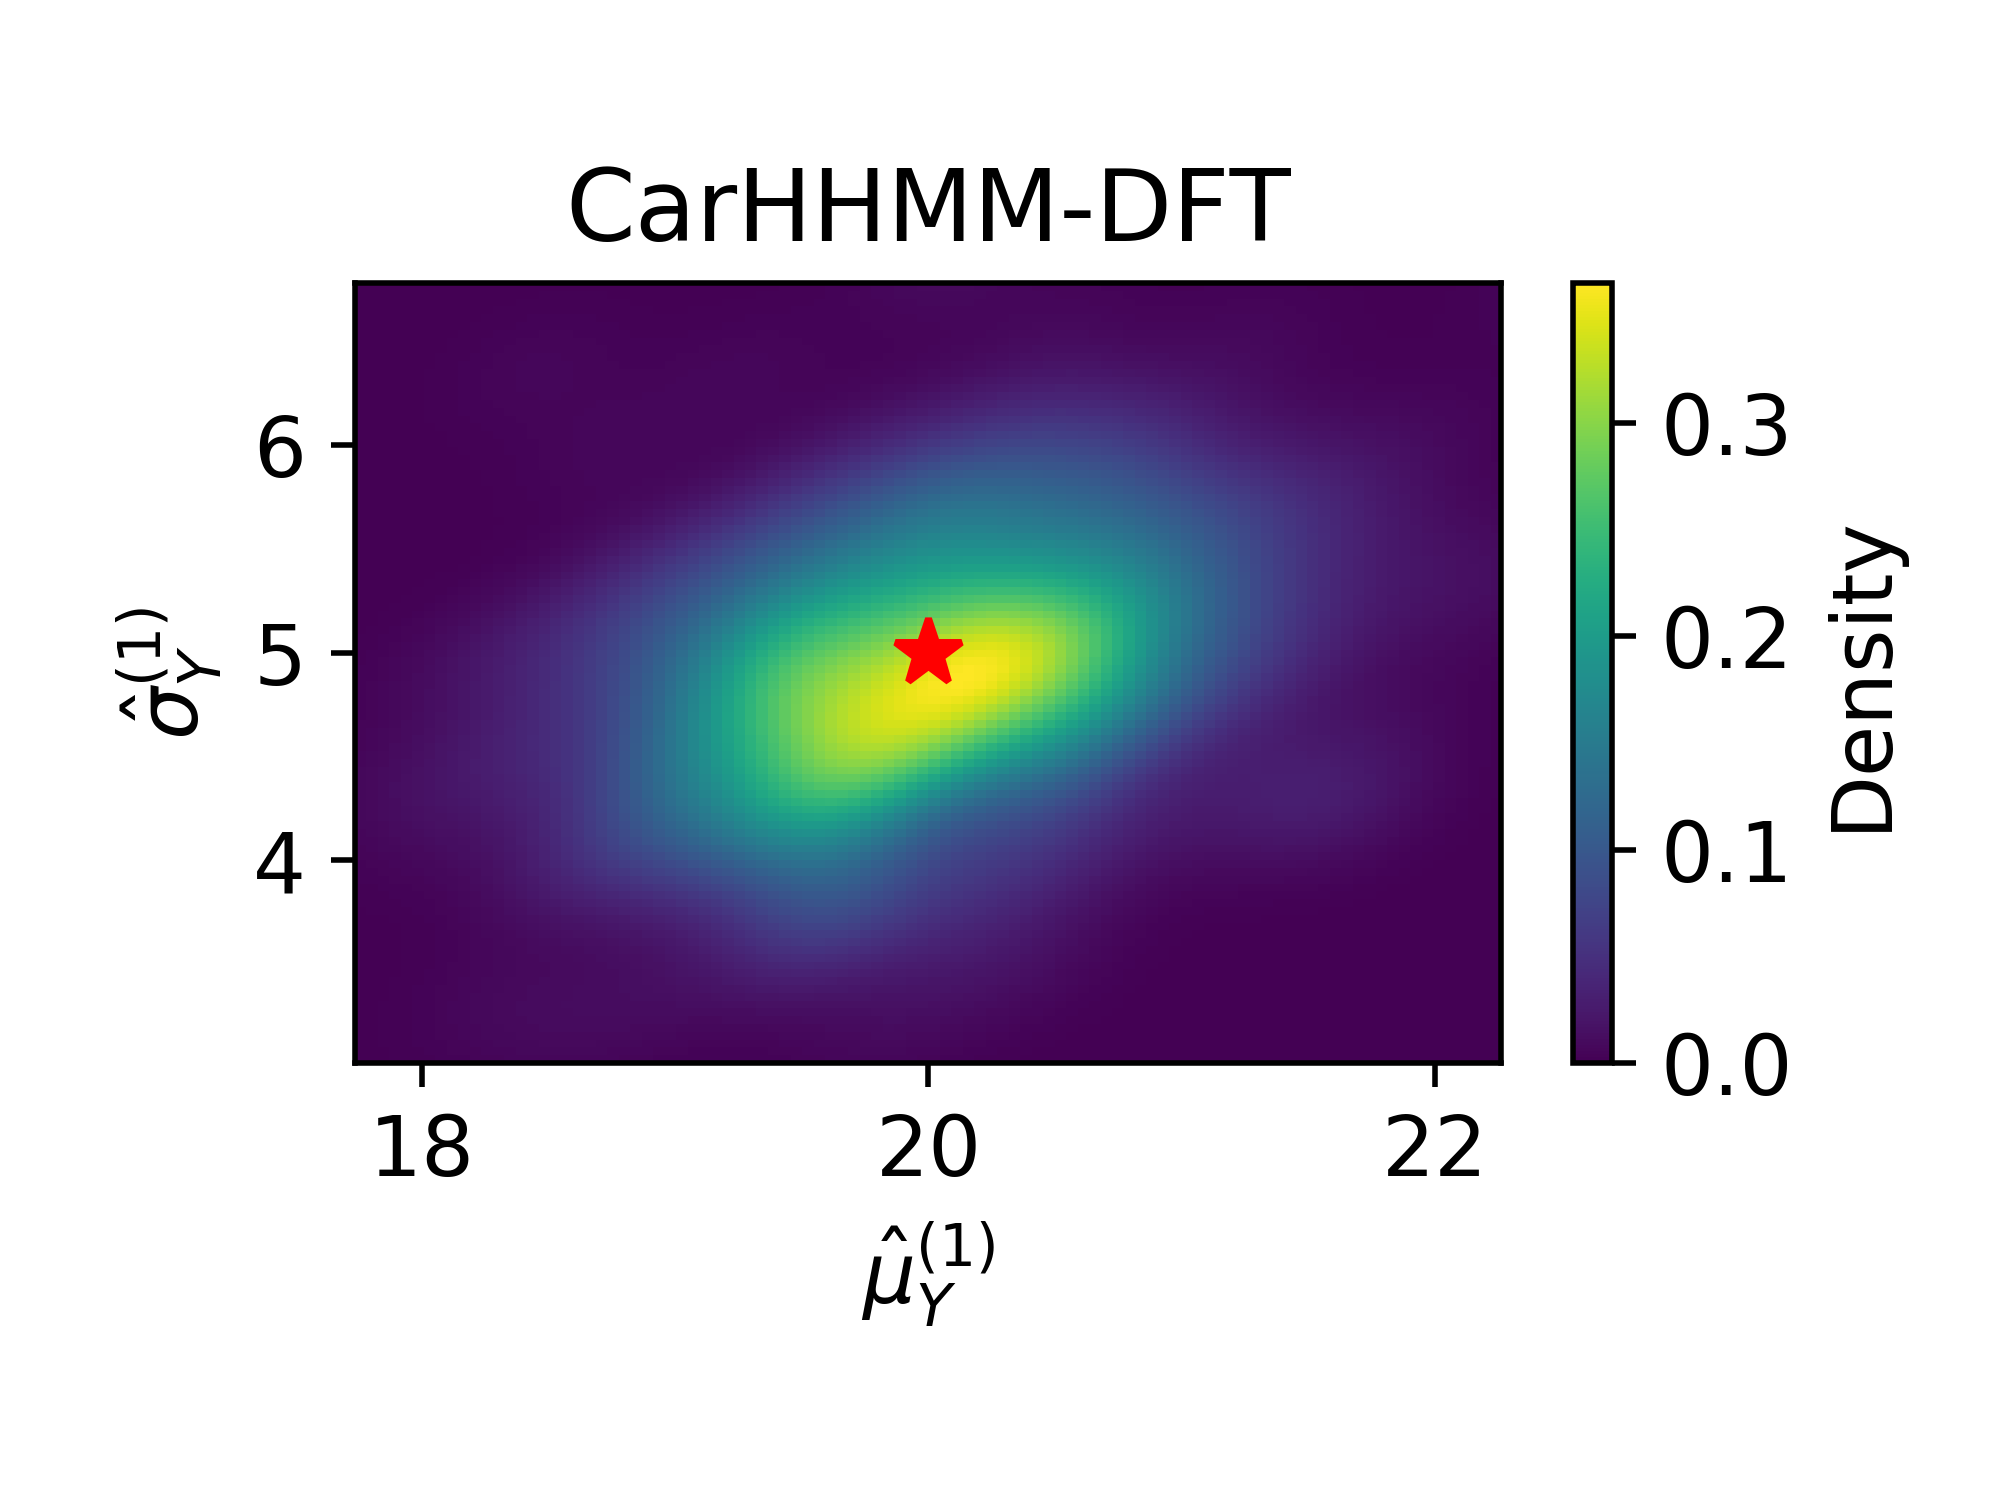
\includegraphics[width=2.25in]{../Plots/hhmm_FV_MLE_density_dive_duration_-1_0.png}
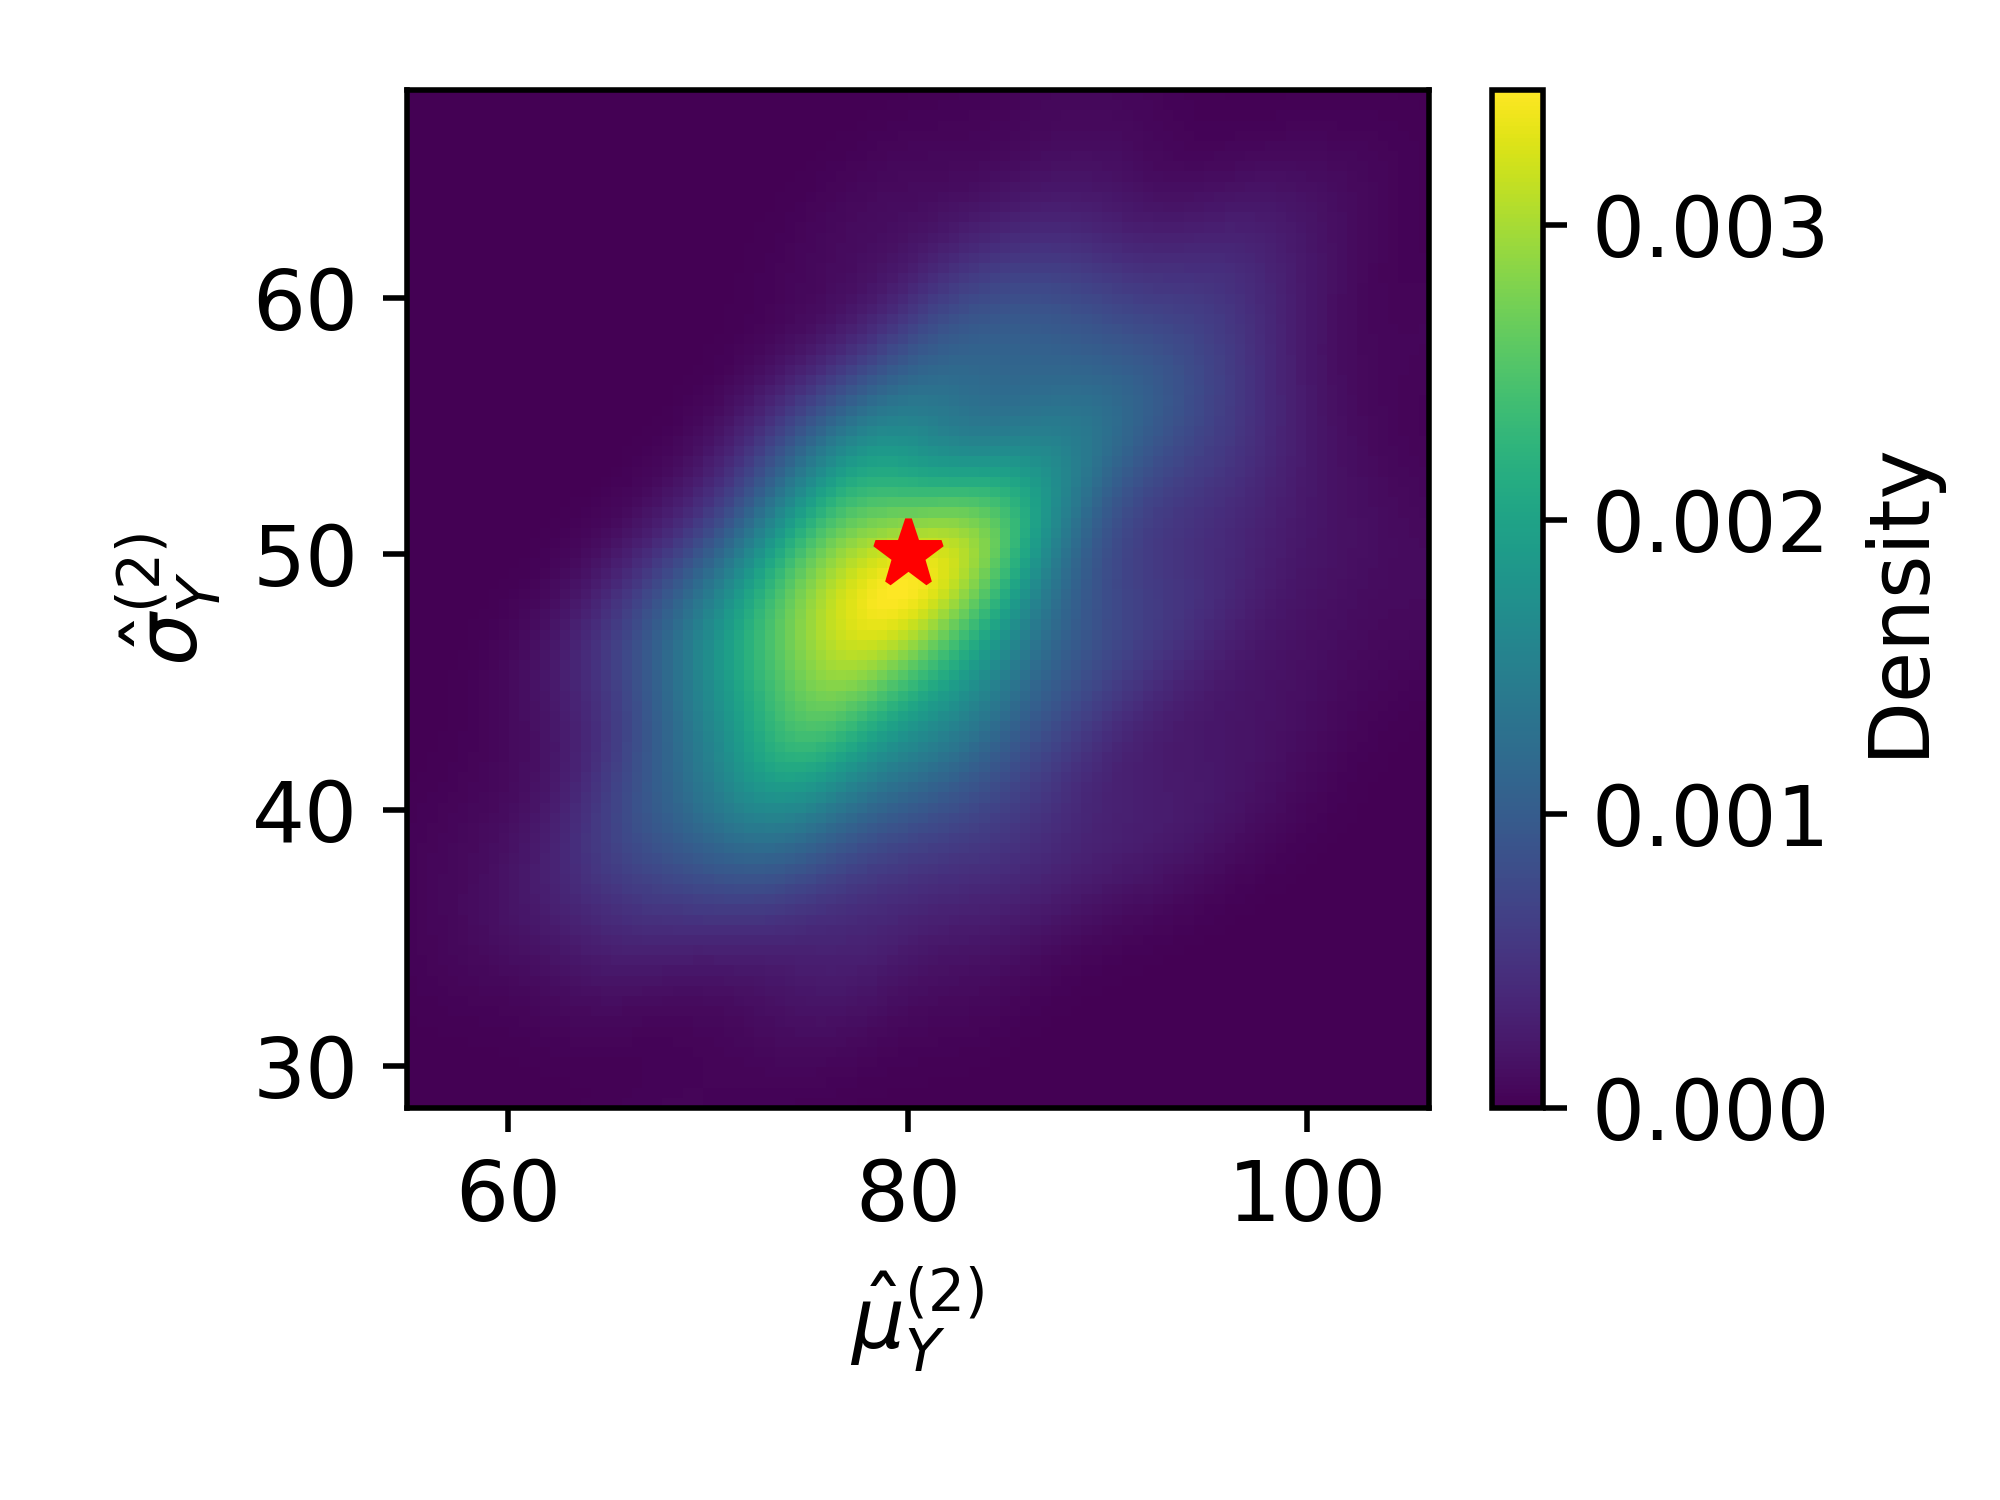
\includegraphics[width=2.25in]{../Plots/hhmm_FV_MLE_density_dive_duration_-1_1.png}
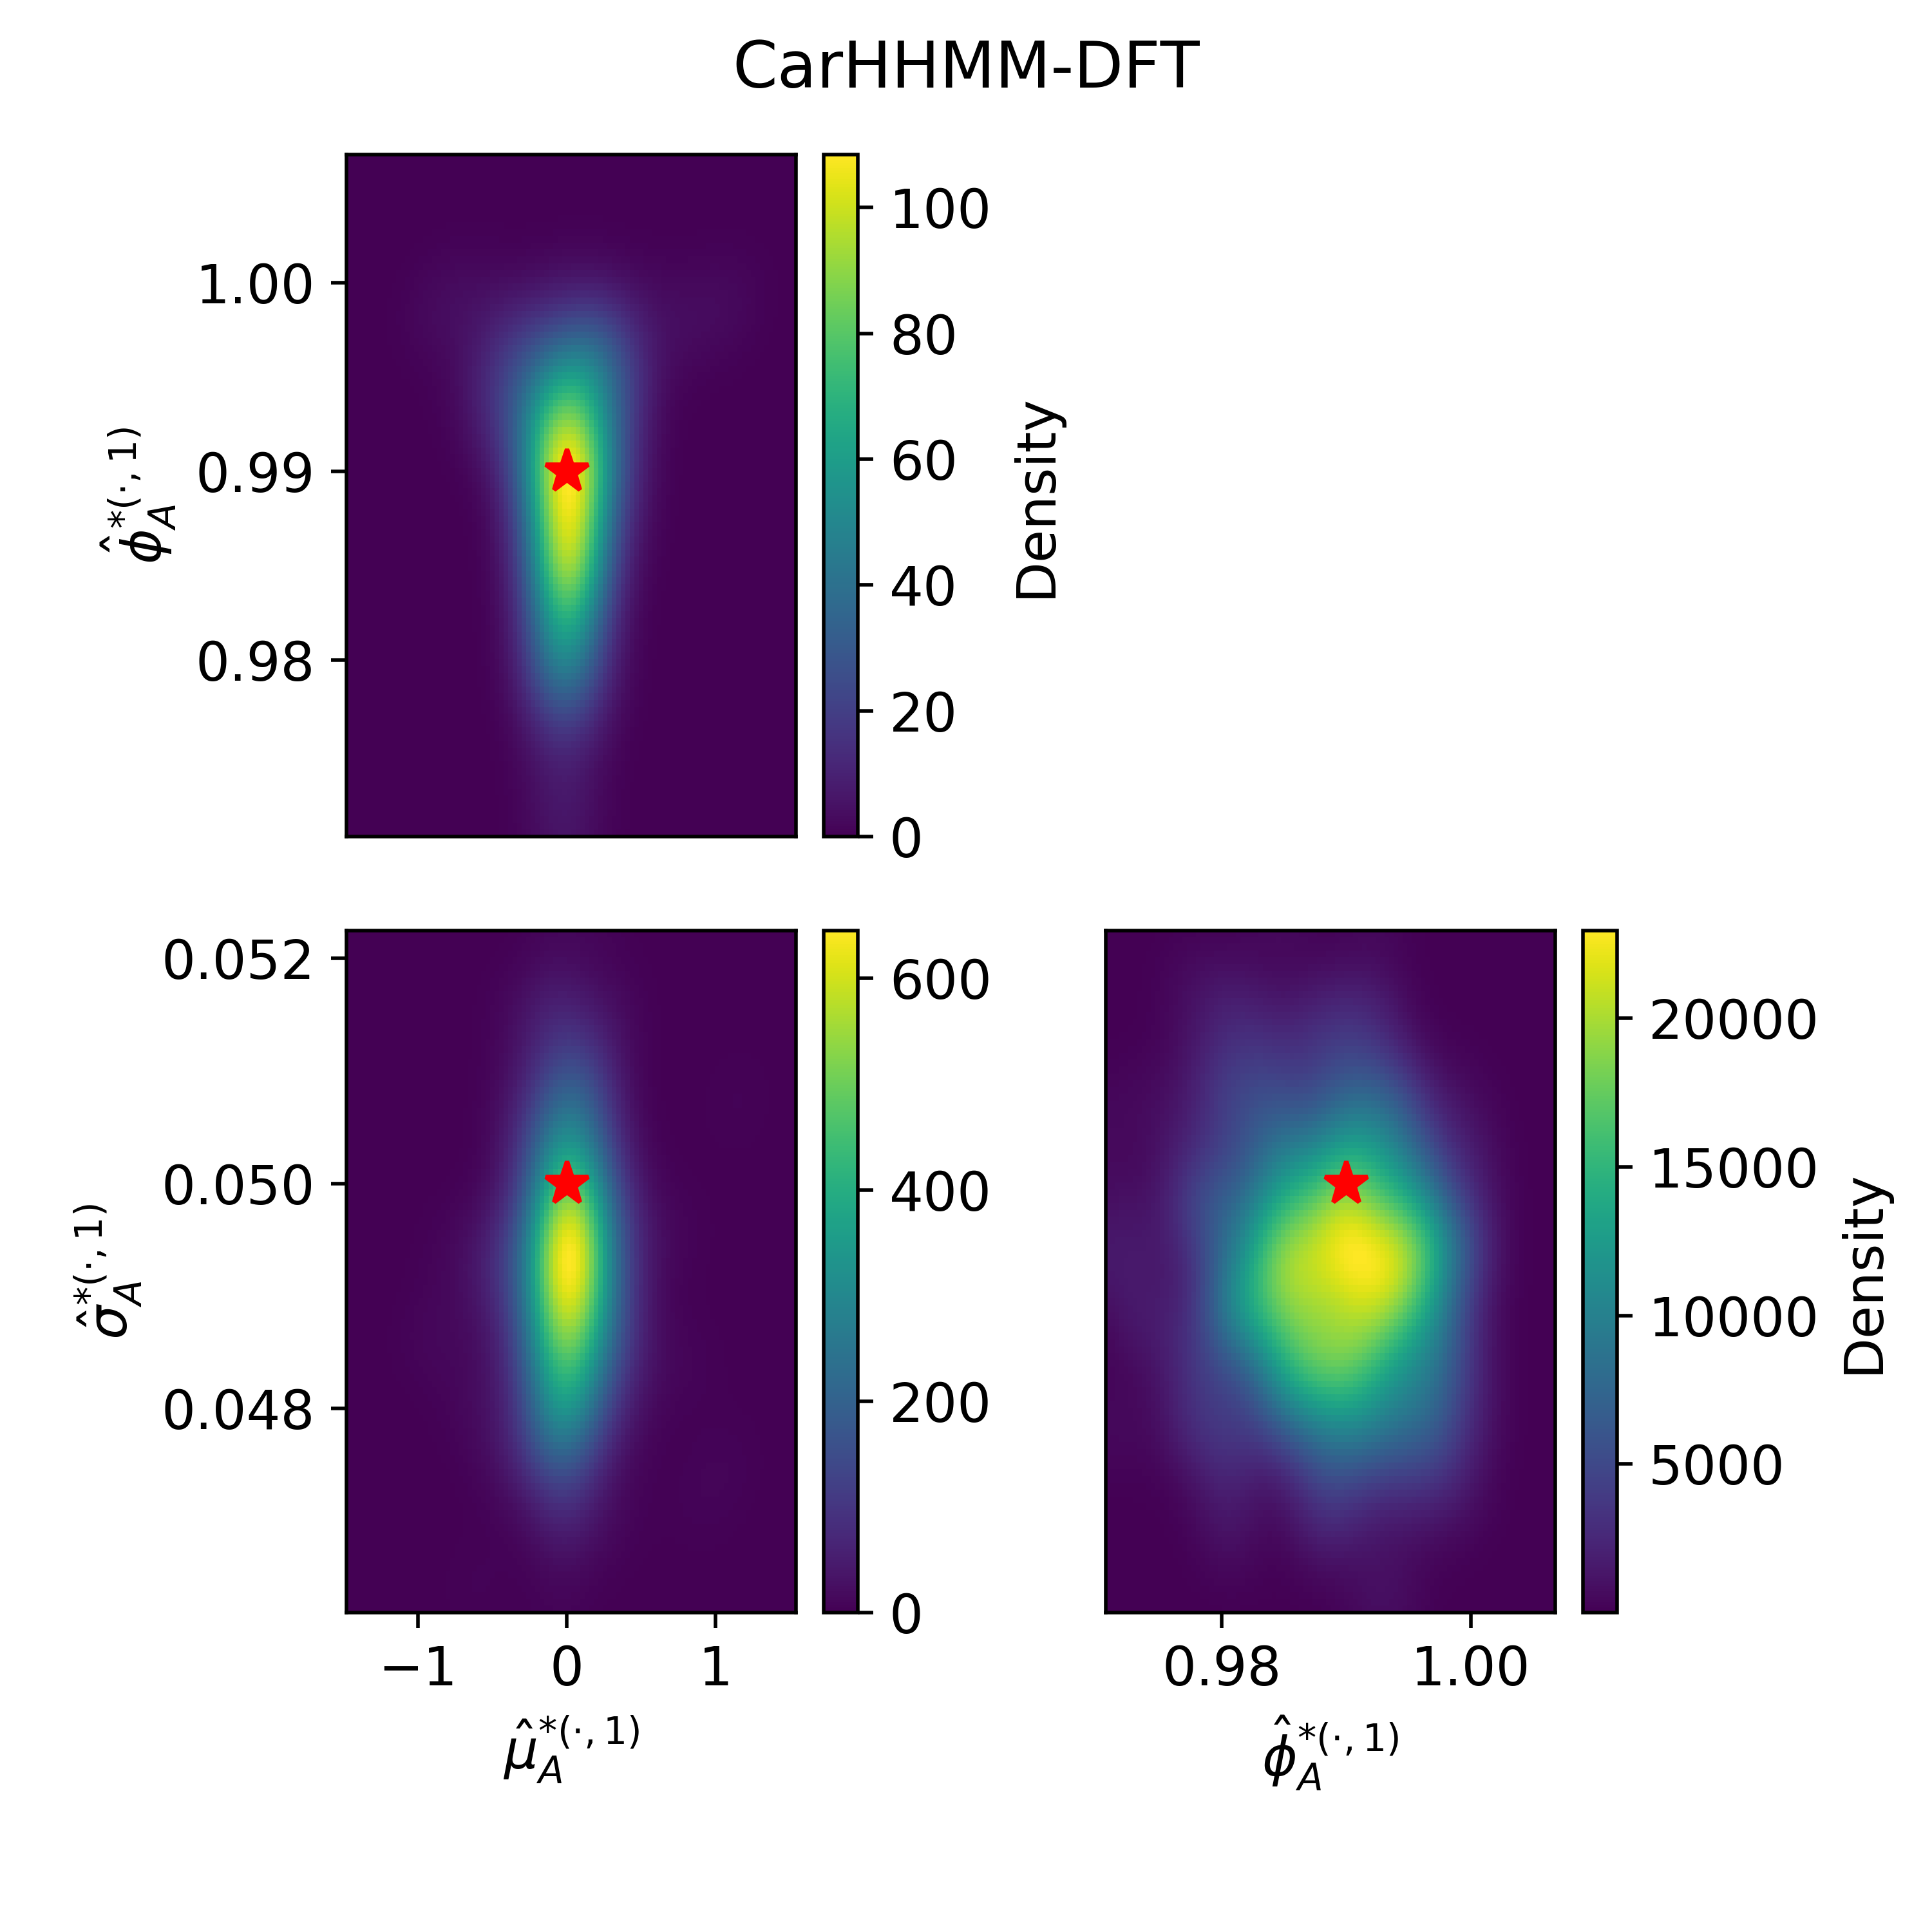
\includegraphics[height=4in]{../Plots/hhmm_FV_MLE_density_A_0_0.png}
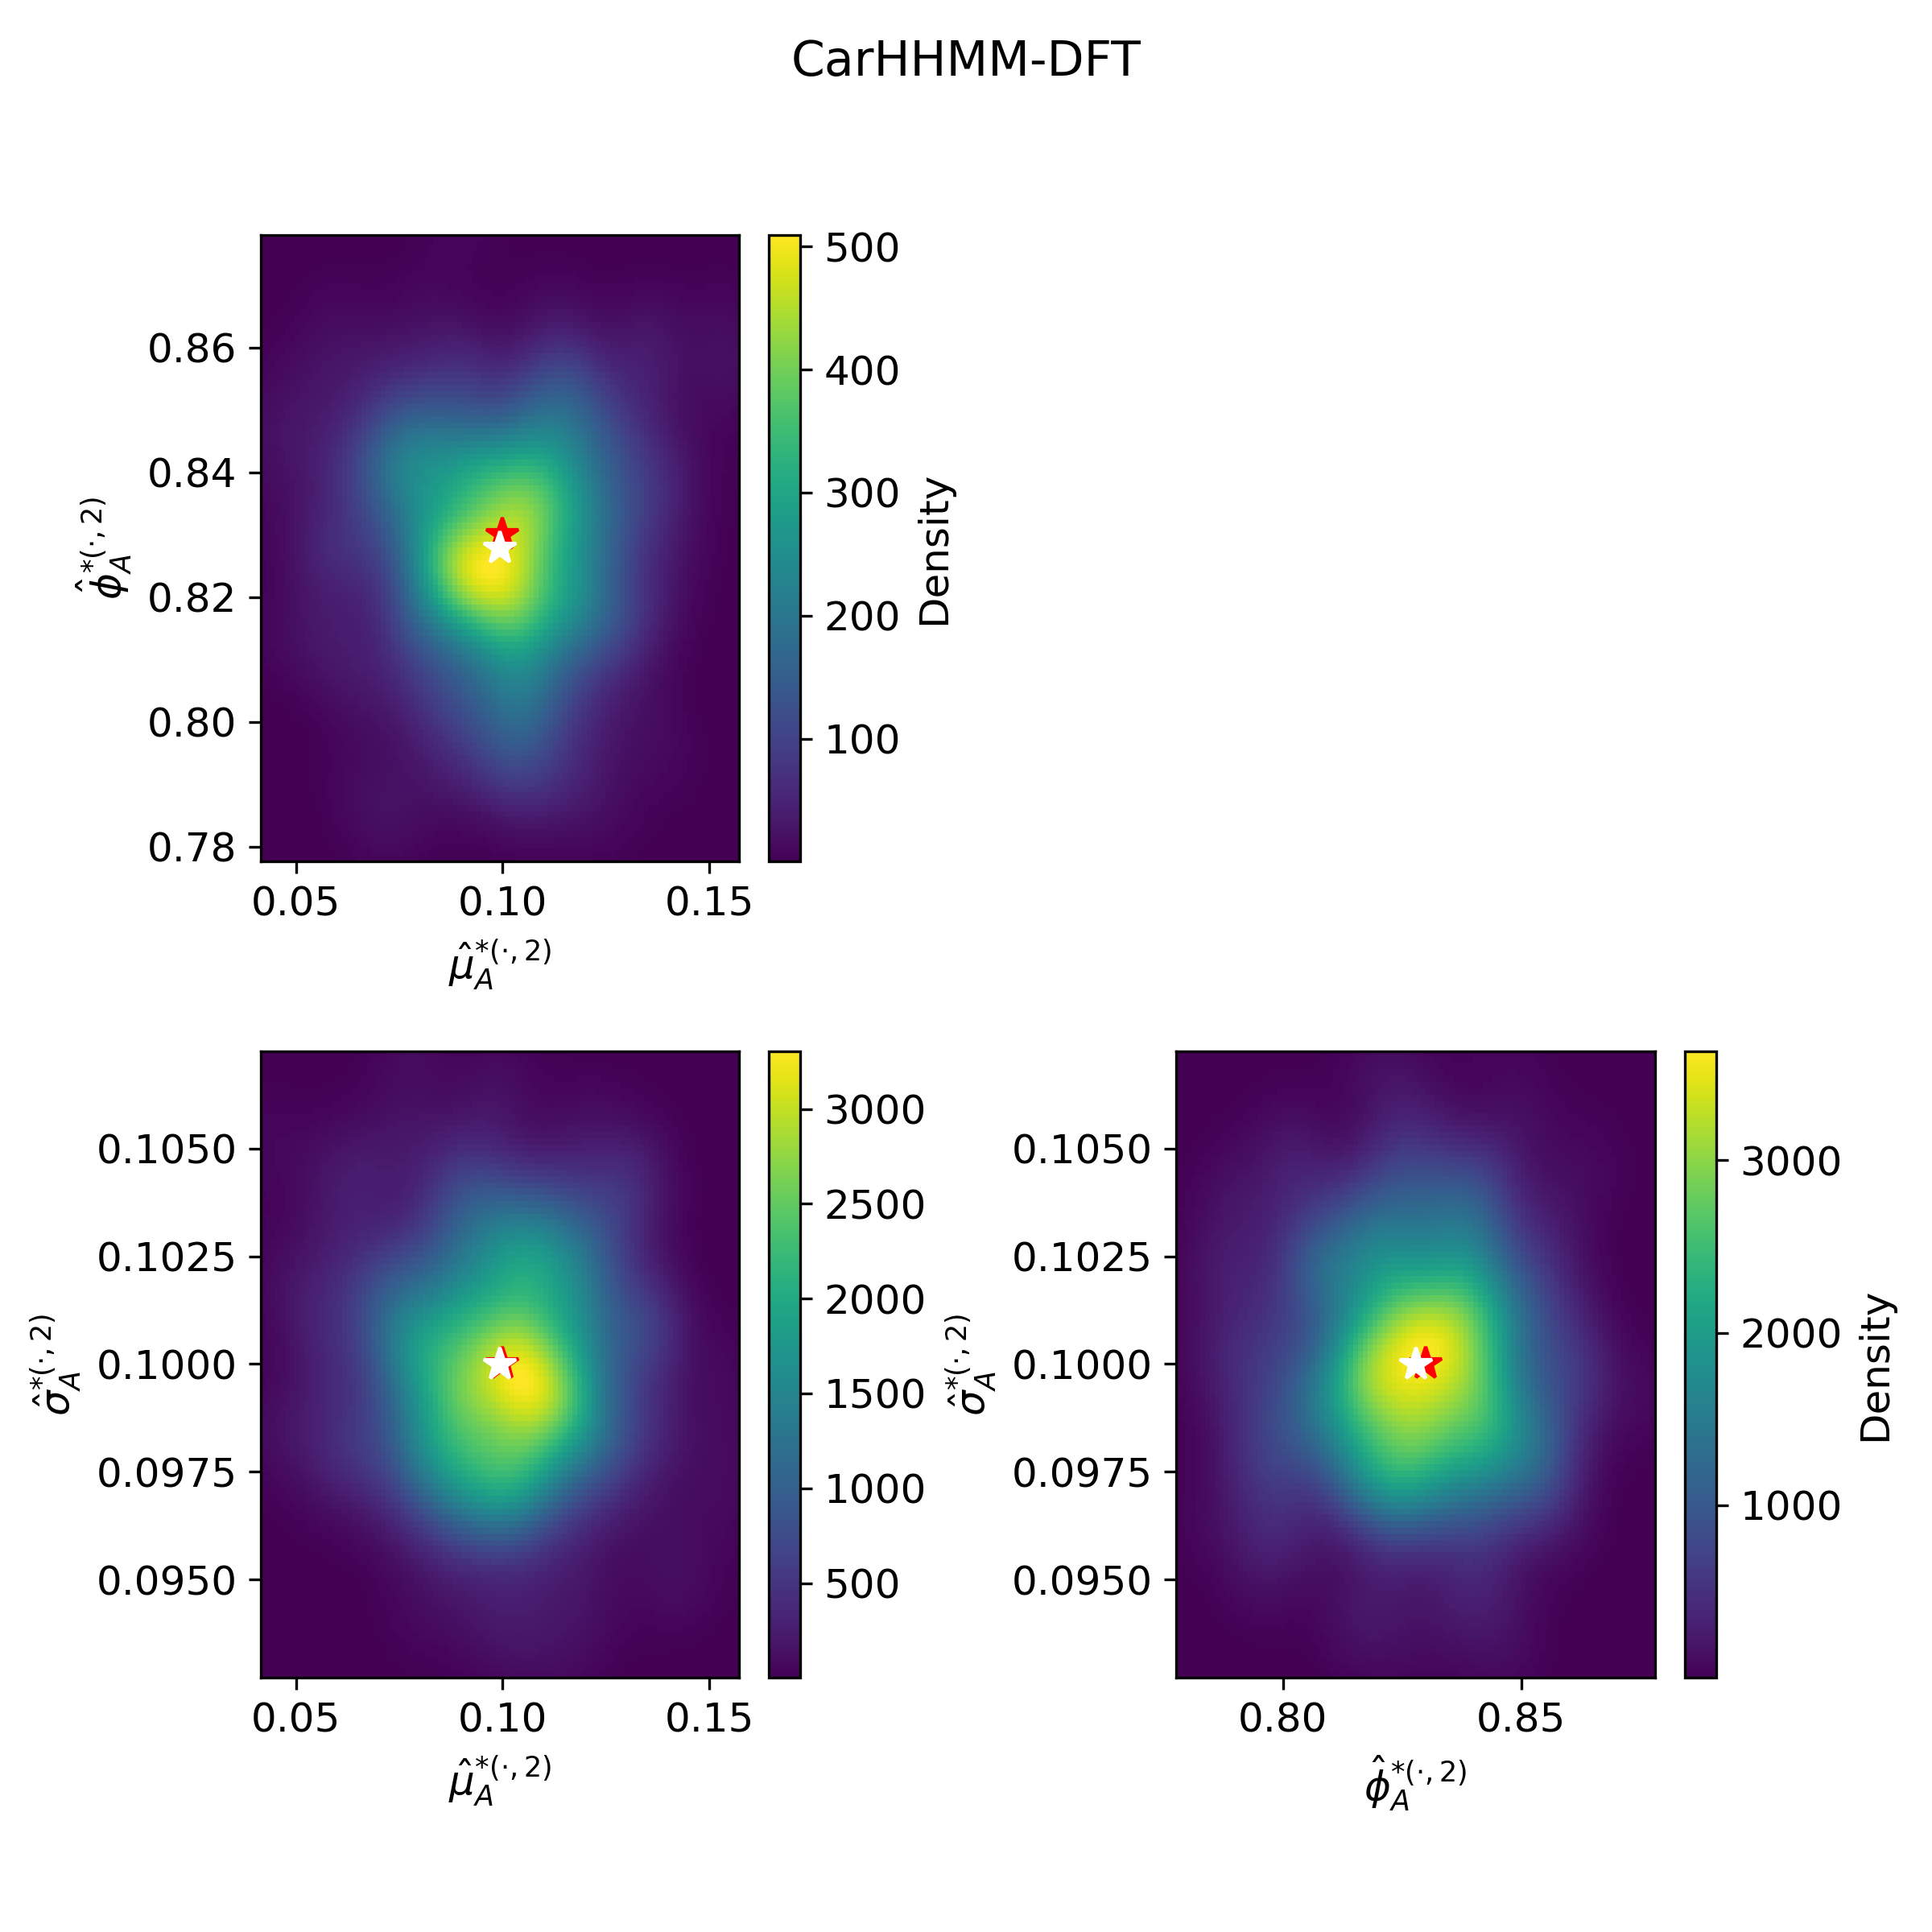
\includegraphics[height=4in]{../Plots/hhmm_FV_MLE_density_A_0_1.png}
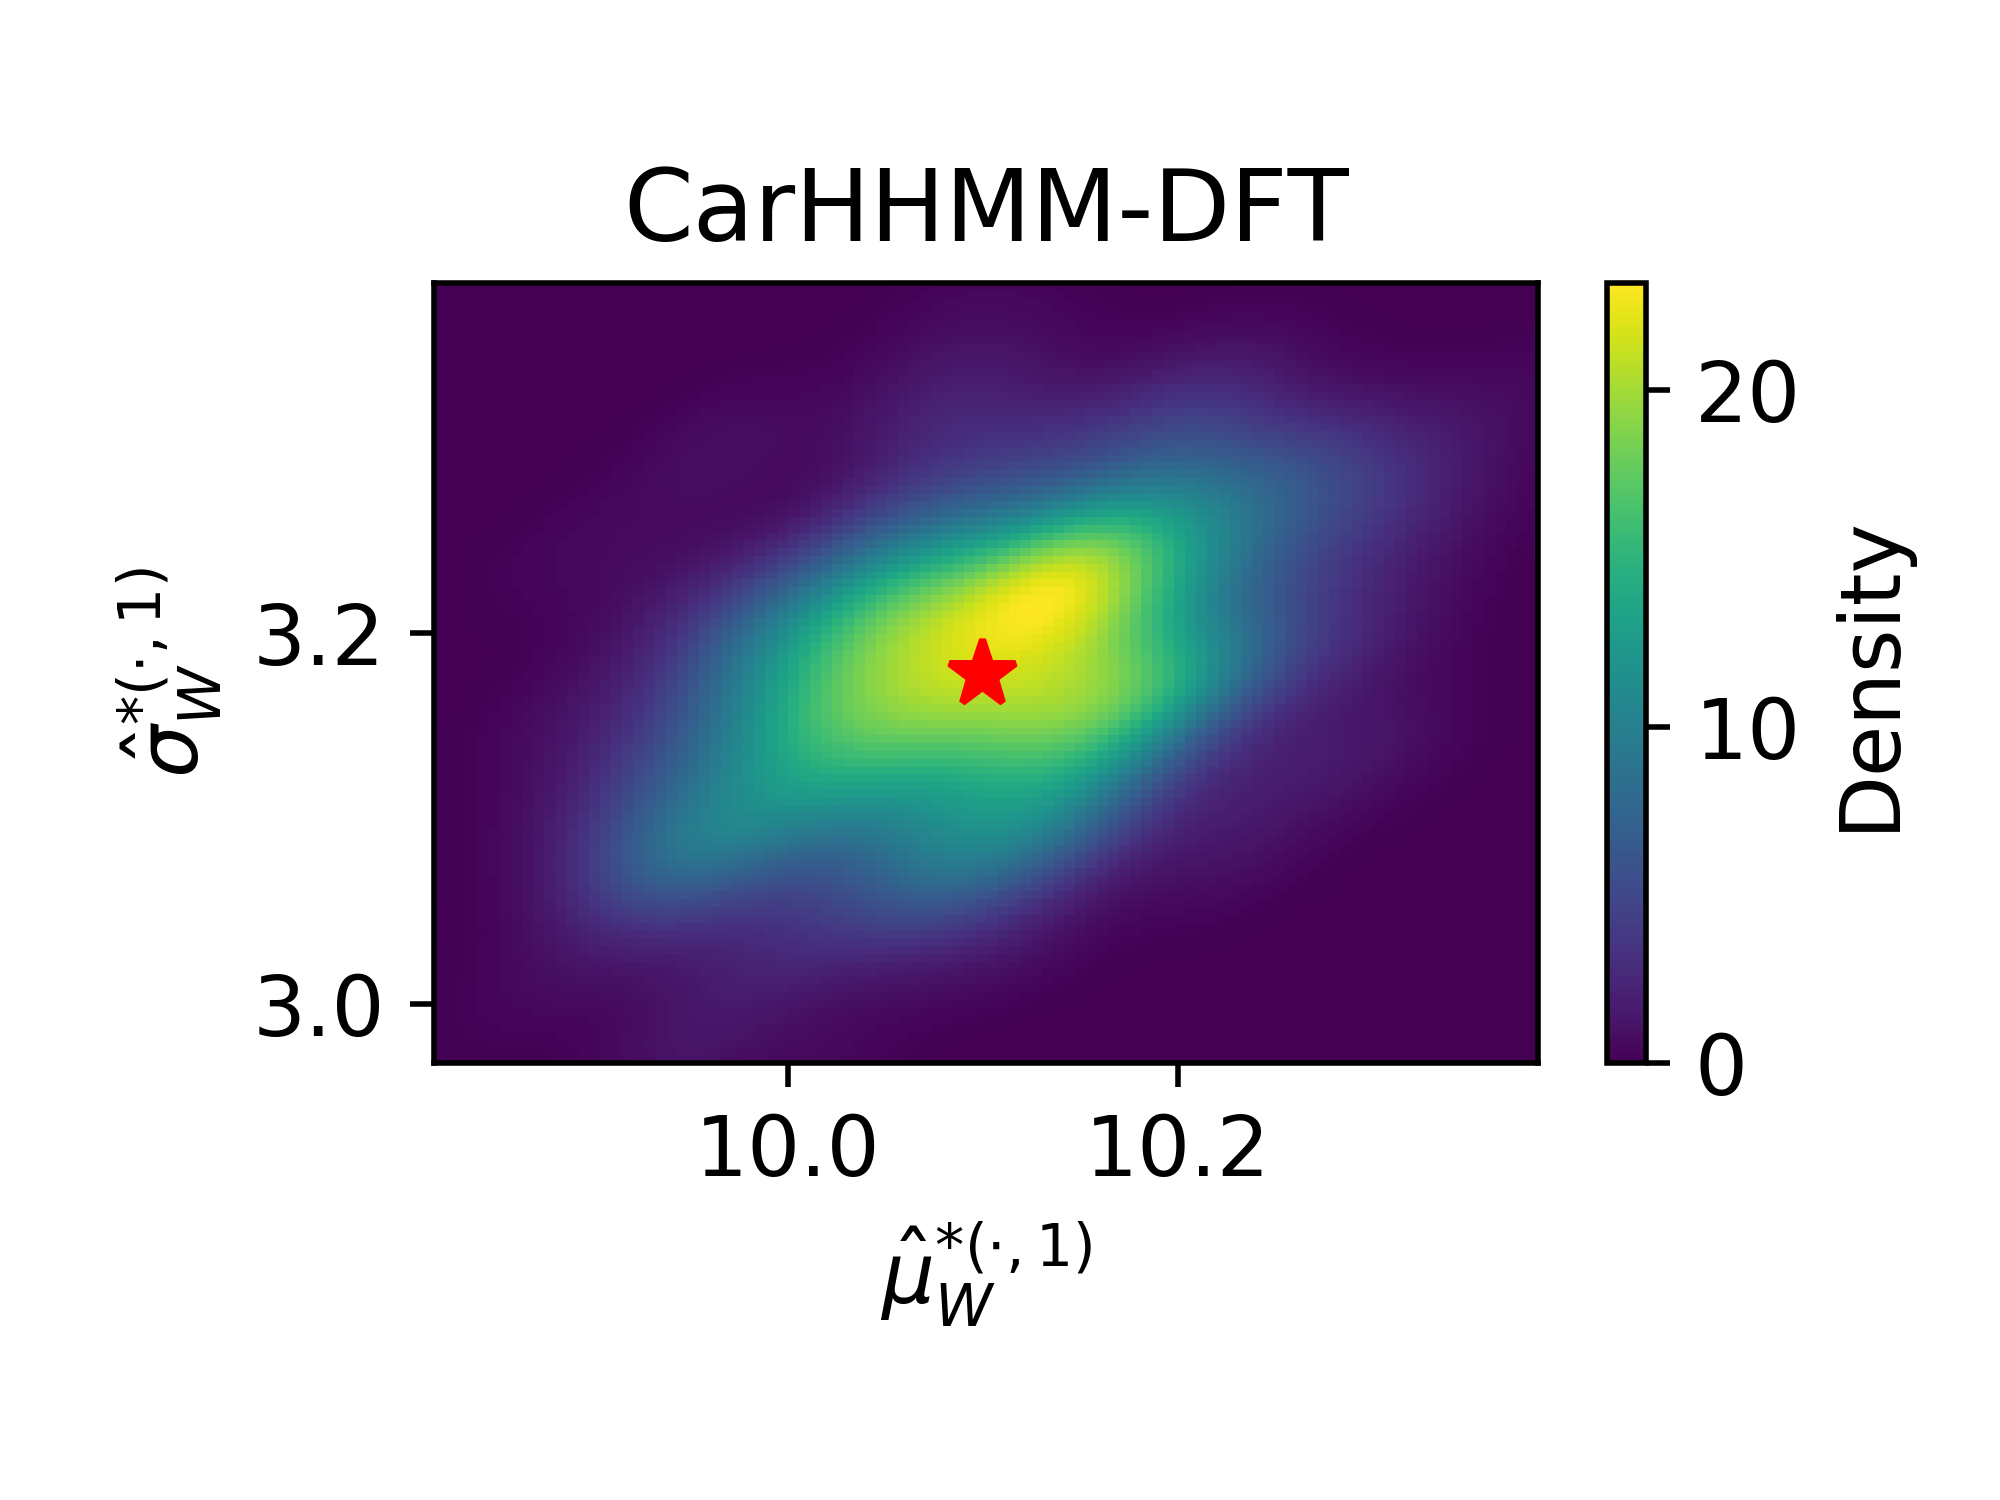
\includegraphics[width=2.25in]{../Plots/hhmm_FV_MLE_density_FoVeDBA_0_0.png}
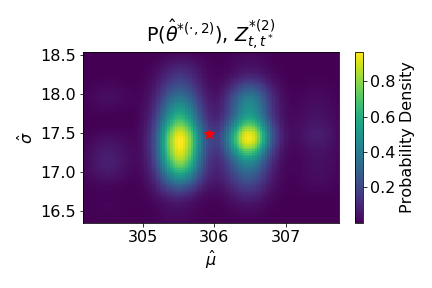
\includegraphics[width=2.25in]{../Plots/hhmm_FV_MLE_density_FoVeDBA_0_1.png}


%%%%%%%%%%%%%%%%%%%%%%%%%%%%%%%%%%%%

\newpage
\subsection{Parameter estimates and standard errors}

%%% Accuracy %%%

Below is a table showing the accuracies and run times for all models. All reported values are averages, and $\pm$ refers to the standard deviation.
\vspace{1cm}

\centering
\scalebox{0.8}{
\begin{tabular}{ccccccc}
Model                      & \multicolumn{1}{c}{Training Time (Minutes)} & \multicolumn{1}{c}{Dive Type} & \multicolumn{1}{c}{Subdive Type} & \multicolumn{1}{c}{Dive Accuracy} & \multicolumn{1}{c}{Subdive Accuracy}  \\ \hline
\multirow{5}{*}{CarHMM-DFT}& \multirow{5}{*}{$15.74 \pm 2.46$}   & Both                          & Both                             & -------------                     & $1.00 \pm 0.00$                       \\
                           &                                    & 1                             & 1                                & \multirow{2}{*}{-------------}    & $1.00 \pm 0.00$                       \\ 
                           &                                    & 1                             & 2                                &                                   & $1.00 \pm 0.00$                       \\ 
                           &                                    & 2                             & 1                                & \multirow{2}{*}{-------------}    & $1.00 \pm 0.00$                       \\ 
                           &                                    & 2                             & 2                                &                                   & $1.00 \pm 0.00$                       \\ \hline 
\multirow{5}{*}{HHMM-DFT}  & \multirow{5}{*}{$82.43 \pm 11.48$}   & Both                          & Both                             & $0.94 \pm 0.02$                   & $1.00 \pm 0.00$                       \\
                           &                                    & 1                             & 1                                & \multirow{2}{*}{$0.94\pm0.03$}    & $1.00 \pm 0.00$                       \\ 
                           &                                    & 1                             & 2                                &                                   & $1.00 \pm 0.00$                       \\ 
                           &                                    & 2                             & 1                                & \multirow{2}{*}{$0.94\pm0.03$}    & $1.00 \pm 0.00$                       \\ 
                           &                                    & 2                             & 2                                &                                   & $1.00 \pm 0.00$                       \\ \hline
\multirow{5}{*}{CarHHMM}   & \multirow{5}{*}{$70.85 \pm 15.89$}   & Both                          & Both                             & $0.91 \pm 0.03$                   & $0.89 \pm 0.02$                       \\
                           &                                    & 1                             & 1                                & \multirow{2}{*}{$0.87\pm0.04$}    & $0.44 \pm 0.12$                       \\ 
                           &                                    & 1                             & 2                                &                                   & $1.00 \pm 0.00$                       \\ 
                           &                                    & 2                             & 1                                & \multirow{2}{*}{$0.95\pm0.03$}    & $0.81 \pm 0.04$                       \\ 
                           &                                    & 2                             & 2                                &                                   & $1.00 \pm 0.00$                       \\ \hline
\multirow{5}{*}{CarHHMM-DFT}& \multirow{5}{*}{$81.22 \pm 16.10$}   & Both                          & Both                             & $0.94 \pm 0.02$                   & $1.00 \pm 0.00$                       \\
                           &                                    & 1                             & 1                                & \multirow{2}{*}{$0.94\pm0.03$}    & $1.00 \pm 0.00$                       \\ 
                           &                                    & 1                             & 2                                &                                   & $1.00 \pm 0.00$                       \\ 
                           &                                    & 2                             & 1                                & \multirow{2}{*}{$0.94\pm0.03$}    & $1.00 \pm 0.00$                       \\ 
                           &                                    & 2                             & 2                                &                                   & $1.00 \pm 0.00$                       \\ \hline
\end{tabular}
}


%%% dive duration %%%
\newpage
Below is a table of estimates and standard errors of parameters for dive duration distribution for all four models. All reported values are averages, except for the Fisher observed standard error, which are medians. $\pm$ refers to the IQR.
\vspace{1cm}

\centering
\scalebox{0.9}{
\begin{tabular}{ccccccc}
Model                      & \multicolumn{1}{c}{Parameter} & \multicolumn{1}{c}{Dive Type} & \multicolumn{1}{c}{Estimate} & \multicolumn{1}{c}{Bias} & \multicolumn{1}{c}{Empirical SE} & \multicolumn{1}{c}{Observed Fischer SE}           \\ \hline
\multirow{4}{*}{CarHMM-DFT}& \multirow{2}{*}{$\mu$}        & 1                             & $49.72$                         & $-0.28$                     & $4.78$                             & $2.47 \pm 0.34$                             \\
                           &                               & ---                           & ---                            & ---                        & ---                                & ---                                         \\
                           & \multirow{2}{*}{$\sigma$}     & 1                             & $39.00$                         & $-7.51$                     & $5.05$                             & $2.50 \pm 0.40$                             \\
                           &                               & ---                           & ---                            & ---                        & ---                                & ---                                         \\ \hline
\multirow{4}{*}{HHMM-DFT}  & \multirow{2}{*}{$\mu$}        & 1                             & $19.99$                         & $-0.01$                     & $0.75$                             & $0.69 \pm 0.11$                             \\
                           &                               & 2                             & $79.85$                         & $-0.15$                     & $8.05$                             & $5.85 \pm 1.10$                             \\
                           & \multirow{2}{*}{$\sigma$}     & 1                             & $4.90$                         & $-0.10$                     & $0.61$                             & $0.53 \pm 0.10$                             \\
                           &                               & 2                             & $48.74$                         & $-1.26$                     & $6.50$                             & $5.15 \pm 1.02$                             \\ \hline
\multirow{4}{*}{CarHHMM}   & \multirow{2}{*}{$\mu$}        & 1                             & $19.91$                         & $-0.09$                     & $0.77$                             & $0.71 \pm 0.12$                             \\
                           &                               & 2                             & $75.80$                         & $-4.20$                     & $7.72$                             & $5.32 \pm 0.98$                             \\
                           & \multirow{2}{*}{$\sigma$}     & 1                             & $4.73$                         & $-0.27$                     & $0.59$                             & $0.55 \pm 0.10$                             \\
                           &                               & 2                             & $49.48$                         & $-0.52$                     & $6.26$                             & $4.79 \pm 0.93$                             \\ \hline
\multirow{4}{*}{CarHHMM-DFT}& \multirow{2}{*}{$\mu$}        & 1                             & $19.99$                         & $-0.01$                     & $0.75$                             & $0.69 \pm 0.12$                             \\
                           &                               & 2                             & $79.85$                         & $-0.15$                     & $8.05$                             & $5.85 \pm 1.10$                             \\
                           & \multirow{2}{*}{$\sigma$}     & 1                             & $4.90$                         & $-0.10$                     & $0.61$                             & $0.53 \pm 0.10$                             \\
                           &                               & 2                             & $48.74$                         & $-1.26$                     & $6.50$                             & $5.15 \pm 1.02$                             
\end{tabular}
}

%%% Acceleration %%%
\newpage
Below is a table of estimates and standard errors of parameters for $Z^{*(1)}_{t,t^*}$ for all four models. All reported values are averages, except for the Fisher observed standard error, which are medians. $\pm$ refers to the IQR.
\vspace{1cm}

\centering
\scalebox{0.7}{
\begin{tabular}{ccccccc}
Model                      & \multicolumn{1}{c}{Parameter} & \multicolumn{1}{c}{Subdive Type} & \multicolumn{1}{c}{Estimate} & \multicolumn{1}{c}{Bias} & \multicolumn{1}{c}{Empirical SE} & \multicolumn{1}{c}{Observed Fischer SE}        \\ \hline
\multirow{6}{*}{CarHMM-DFT}& \multirow{2}{*}{$\mu$}        & 1                             & $0.00$                         & $0.00$                     & $0.00$                             & $0.14 \pm 0.13$                             \\
                           &                               & 2                             & $0.00$                         & $0.00$                     & $0.01$                             & $0.06 \pm 0.02$                             \\
                           & \multirow{2}{*}{$\sigma$}     & 1                             & $0.05$                         & $-0.00$                     & $0.00$                             & $0.00 \pm 0.00$                             \\
                           &                               & 2                             & $0.10$                         & $-0.00$                     & $0.00$                             & $0.00 \pm 0.00$                             \\ 
                           & \multirow{2}{*}{$\phi$}       & 1                             & $0.99$                         & $-0.00$                     & $0.01$                             & $0.01 \pm 0.00$                             \\
                           &                               & 2                             & $0.95$                         & $-0.00$                     & $0.01$                             & $0.01 \pm 0.00$                             \\ \hline
\multirow{6}{*}{HHMM-DFT}  & \multirow{2}{*}{$\mu$}        & 1                             & $-0.01$                         & $-0.01$                     & $0.02$                             & $0.01 \pm 0.00$                             \\
                           &                               & 2                             & $-0.00$                         & $-0.00$                     & $0.02$                             & $0.01 \pm 0.00$                             \\
                           & \multirow{2}{*}{$\sigma$}     & 1                             & $0.25$                         & $0.20$                     & $0.04$                             & $0.00 \pm 0.00$                             \\
                           &                               & 2                             & $0.24$                         & $0.14$                     & $0.03$                             & $0.00 \pm 0.00$                             \\ 
                           & \multirow{2}{*}{$\phi$}       & 1                             & ------                         & ------                     & ------                             & ------                                      \\
                           &                               & 2                             & ------                         & ------                     & ------                             & ------                                      \\ \hline
\multirow{6}{*}{CarHHMM}   & \multirow{2}{*}{$\mu$}        & 1                             & $0.00$                         & $0.00$                     & $0.00$                             & $0.08 \pm 0.04$                             \\
                           &                               & 2                             & $-0.01$                         & $-0.01$                     & $0.01$                             & $0.01 \pm 0.00$                             \\
                           & \multirow{2}{*}{$\sigma$}     & 1                             & $0.05$                         & $0.00$                     & $0.04$                             & $0.00 \pm 0.00$                             \\
                           &                               & 2                             & $0.27$                         & $0.17$                     & $0.01$                             & $0.00 \pm 0.00$                             \\ 
                           & \multirow{2}{*}{$\phi$}       & 1                             & $0.97$                         & $-0.02$                     & $0.10$                             & $0.00 \pm 0.00$                             \\
                           &                               & 2                             & $0.49$                         & $-0.46$                     & $0.05$                             & $0.02 \pm 0.00$                             \\ \hline
\multirow{6}{*}{CarHHMM-DFT}& \multirow{2}{*}{$\mu$}        & 1                             & $0.00$                         & $0.00$                     & $0.00$                             & $0.13 \pm 0.12$                             \\
                           &                               & 2                             & $0.00$                         & $0.00$                     & $0.00$                             & $0.06 \pm 0.02$                             \\
                           & \multirow{2}{*}{$\sigma$}     & 1                             & $0.05$                         & $-0.00$                     & $0.00$                             & $0.00 \pm 0.00$                             \\
                           &                               & 2                             & $0.10$                         & $-0.00$                     & $0.00$                             & $0.00 \pm 0.00$                             \\ 
                           & \multirow{2}{*}{$\phi$}       & 1                             & $0.99$                         & $-0.00$                     & $0.01$                             & $0.01 \pm 0.00$                             \\
                           &                               & 2                             & $0.95$                         & $-0.00$                     & $0.01$                             & $0.01 \pm 0.00$                             \\ \hline
\end{tabular}
}


%%% FoVeDBA %%%
\newpage
Below is a table of estimates and standard errors of parameters for $Z^{*(2)}_{t,t^*}$ for all four models. All reported values are averages, except for the Fisher observed standard error, which are medians. $\pm$ refers to the IQR.
\vspace{1cm}

\centering
\scalebox{0.8}{
\begin{tabular}{ccccccc}
Model                      & \multicolumn{1}{c}{Parameter} & \multicolumn{1}{c}{Subdive Type} & \multicolumn{1}{c}{Estimate} & \multicolumn{1}{c}{Bias} & \multicolumn{1}{c}{Empirical SE} & \multicolumn{1}{c}{Observed Fischer SE}        \\ \hline
\multirow{4}{*}{CarHMM-DFT}& \multirow{2}{*}{$\mu$}        & 1                             & $10.10$                         & $-0.00$                     & $0.09$                             & $0.08 \pm 0.01$                             \\
                           &                               & 2                             & $305.97$                         & $0.03$                     & $0.54$                             & $0.51 \pm 0.03$                             \\
                           & \multirow{2}{*}{$\sigma$}     & 1                             & $3.18$                         & $-0.00$                     & $0.07$                             & $0.06 \pm 0.01$                             \\
                           &                               & 2                             & $17.46$                         & $-0.03$                     & $0.37$                             & $0.36 \pm 0.02$                             \\ \hline
\multirow{4}{*}{HHMM-DFT}  & \multirow{2}{*}{$\mu$}        & 1                             & $10.10$                         & $-0.00$                     & $0.09$                             & $0.08 \pm 0.01$                             \\
                           &                               & 2                             & $305.97$                         & $0.03$                     & $0.54$                             & $0.51 \pm 0.03$                             \\
                           & \multirow{2}{*}{$\sigma$}     & 1                             & $3.18$                         & $-0.00$                     & $0.07$                             & $0.06 \pm 0.01$                             \\
                           &                               & 2                             & $17.46$                         & $-0.03$                     & $0.37$                             & $0.36 \pm 0.02$                             \\ \hline
\multirow{4}{*}{CarHHMM}   & \multirow{2}{*}{$\mu$}        & 1                             & ------                         & ------                     & ------                             & ------                                      \\
                           &                               & 2                             & ------                         & ------                     & ------                             & ------                                      \\
                           & \multirow{2}{*}{$\sigma$}     & 1                             & ------                         & ------                     & ------                             & ------                                      \\
                           &                               & 2                             & ------                         & ------                     & ------                             & ------                                      \\ \hline
\multirow{4}{*}{CarHHMM-DFT}& \multirow{2}{*}{$\mu$}        & 1                             & $10.10$                         & $-0.00$                     & $0.09$                             & $0.08 \pm 0.01$                             \\
                           &                               & 2                             & $305.97$                         & $0.03$                     & $0.54$                             & $0.51 \pm 0.03$                             \\
                           & \multirow{2}{*}{$\sigma$}     & 1                             & $3.18$                         & $-0.00$                     & $0.07$                             & $0.06 \pm 0.01$                             \\
                           &                               & 2                             & $17.46$                         & $-0.03$                     & $0.37$                             & $0.36 \pm 0.02$                             
\end{tabular}
}

% Gamma
\newpage
Below is a table of estimates and standard errors of $\Gamma$ and $\Gamma^*$ for all four models. All reported values are averages except for the observed fisher SE, which is a median. $\pm$ refers to the IQR.
\vspace{1cm}

\centering
\scalebox{0.7}{
\begin{tabular}{ccccccc}
Model                        & \multicolumn{1}{c}{Parameter} & \multicolumn{1}{c}{Estimate}   & \multicolumn{1}{c}{Bias} & \multicolumn{1}{c}{Empirical SE} & \multicolumn{1}{c}{Observed Fischer SE}     \\ \hline
\multirow{6}{*}{HHMM-DFT}    & $\Gamma_{12}$                 & $0.50$                         & $-0.00$                   & $0.03$                           & $0.08 \pm 0.01$                             \\
                             & $\Gamma_{21}$                 & $0.50$                         & $-0.00$                   & $0.03$                           & $0.08 \pm 0.01$                             \\
                             & $\Gamma^{*(1)}_{12}$          & $0.50$                         & $0.00$                   & $0.00$                           & $0.07 \pm 0.01$                             \\
                             & $\Gamma^{*(1)}_{21}$          & $0.10$                         & $0.00$                   & $0.02$                           & $0.02 \pm 0.00$                             \\
                             & $\Gamma^{*(2)}_{12}$          & $0.20$                         & $-0.00$                   & $0.01$                           & $0.01 \pm 0.00$                             \\
                             & $\Gamma^{*(2)}_{21}$          & $0.30$                         & $-0.00$                   & $0.02$                           & $0.02 \pm 0.00$                             \\ \hline
\multirow{6}{*}{CarHMM-DFT}  & $\Gamma_{12}$                 & ------                         & ------                   & ------                           & ------                                      \\
                             & $\Gamma_{21}$                 & ------                         & ------                   & ------                           & ------                                      \\
                             & $\Gamma^{*(1)}_{12}$          & $0.23$                         & ------                   & $0.01$                           & $0.00 \pm 0.00$                             \\
                             & $\Gamma^{*(1)}_{21}$          & $0.23$                         & ------                   & $0.02$                           & $0.00 \pm 0.00$                             \\
                             & $\Gamma^{*(2)}_{12}$          & ------                         & ------                   & ------                           & ------                                      \\
                             & $\Gamma^{*(2)}_{21}$          & ------                         & ------                   & ------                           & ------                                      \\ \hline
\multirow{6}{*}{CarHHMM}     & $\Gamma_{12}$                 & $0.49$                         & $-0.01$                   & $0.02$                           & $0.08 \pm 0.01$                             \\
                             & $\Gamma_{21}$                 & $0.50$                         & $0.00$                   & $0.02$                           & $0.08 \pm 0.01$                             \\
                             & $\Gamma^{*(1)}_{12}$          & $0.50$                         & $-0.00$                   & $0.00$                           & $0.23 \pm 0.19$                             \\
                             & $\Gamma^{*(1)}_{21}$          & $0.04$                         & $-0.06$                   & $0.02$                           & $0.01 \pm 0.00$                             \\
                             & $\Gamma^{*(2)}_{12}$          & $0.11$                         & $-0.09$                   & $0.02$                           & $0.01 \pm 0.00$                             \\
                             & $\Gamma^{*(2)}_{21}$          & $0.11$                         & $-0.19$                   & $0.03$                           & $0.01 \pm 0.00$                             \\ \hline
\multirow{6}{*}{CarHHMM-DFT} & $\Gamma_{12}$                 & $0.50$                         & $-0.00$                   & $0.03$                           & $0.08 \pm 0.01$                             \\
                             & $\Gamma_{21}$                 & $0.50$                         & $-0.00$                   & $0.03$                           & $0.08 \pm 0.01$                             \\
                             & $\Gamma^{*(1)}_{12}$          & $0.50$                         & $0.00$                   & $0.00$                           & $0.07 \pm 0.01$                             \\
                             & $\Gamma^{*(1)}_{21}$          & $0.10$                         & $0.00$                   & $0.02$                           & $0.02 \pm 0.00$                             \\
                             & $\Gamma^{*(2)}_{12}$          & $0.20$                         & $-0.00$                   & $0.01$                           & $0.01 \pm 0.00$                             \\
                             & $\Gamma^{*(2)}_{21}$          & $0.30$                         & $-0.00$                   & $0.02$                           & $0.02 \pm 0.00$                             \\ \hline

\end{tabular}
}

\newpage
\section{Case Study Results}
\subsection{Model selection- lag plots}

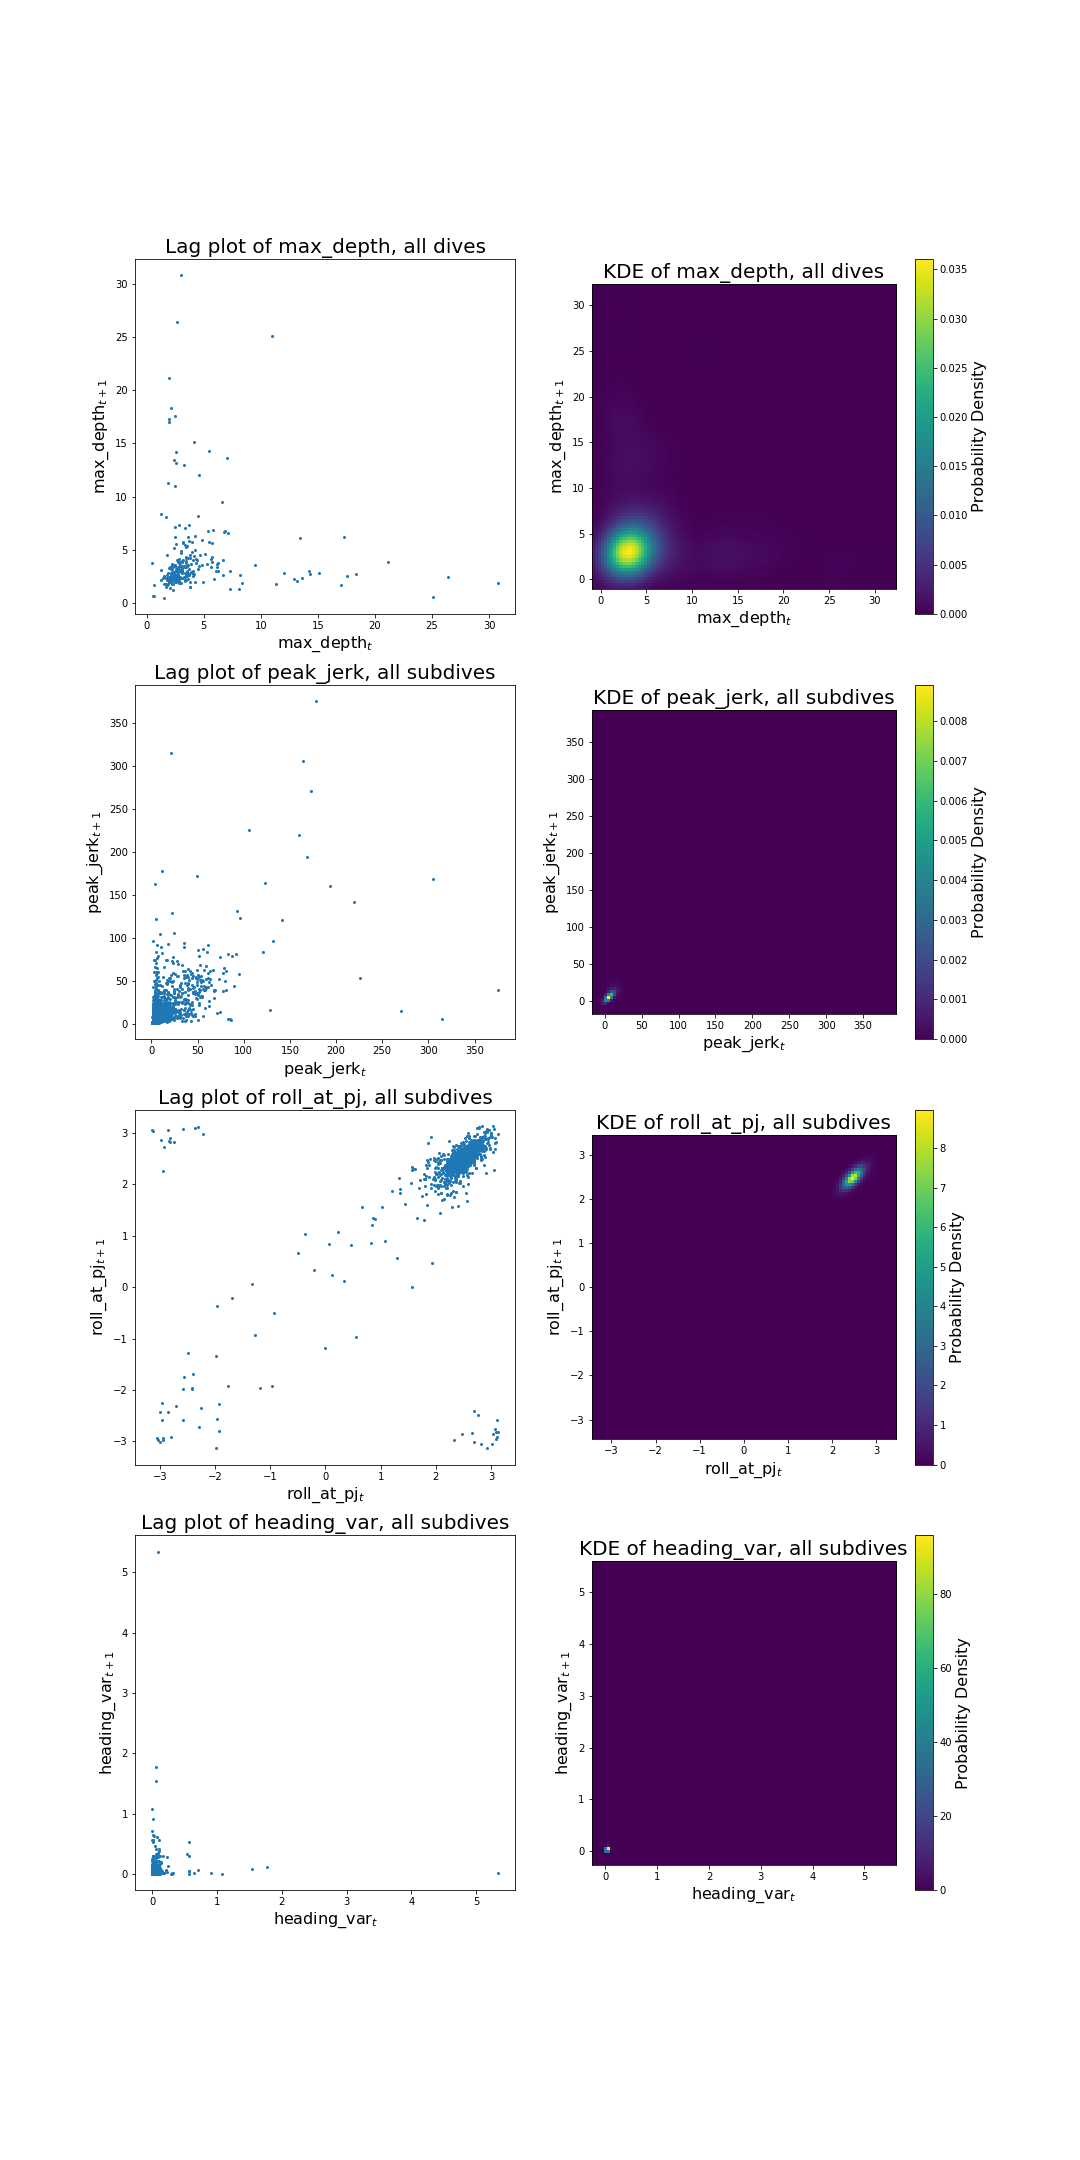
\includegraphics[height=7in]{../Plots/lagplot.png}

\subsection{Results- decoded state probabilities}

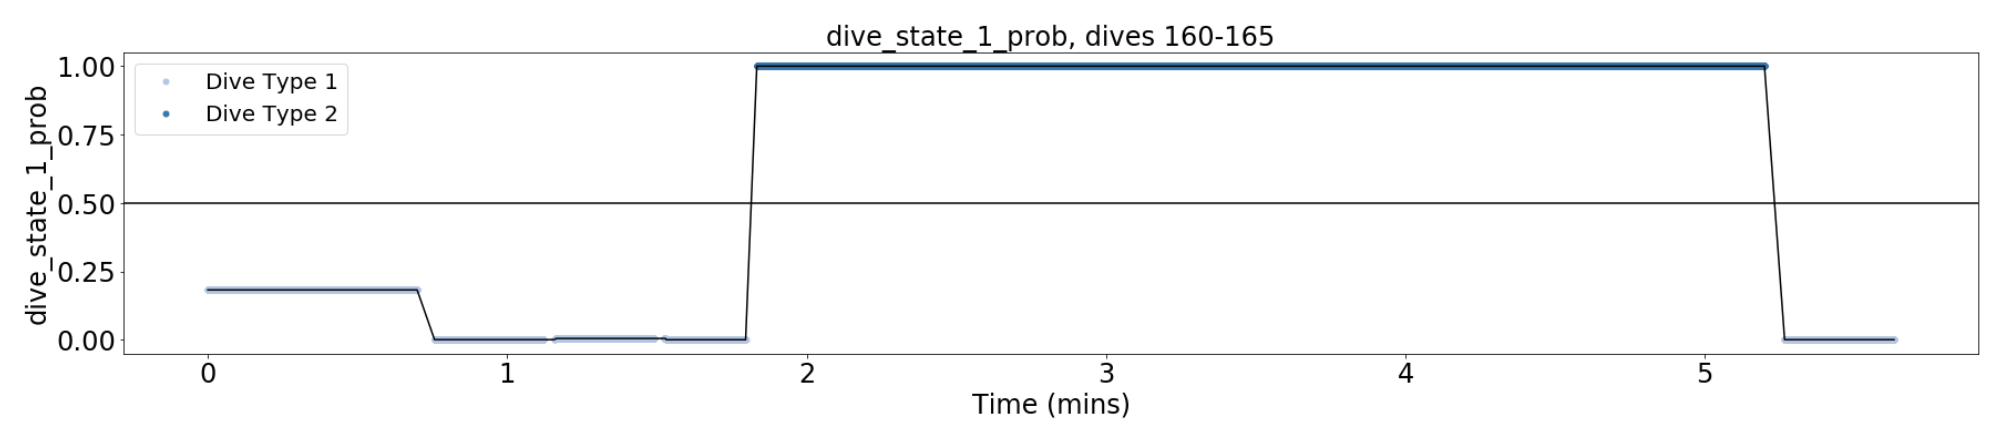
\includegraphics[width=5in]{../Plots/Coarse_state_probs.png}
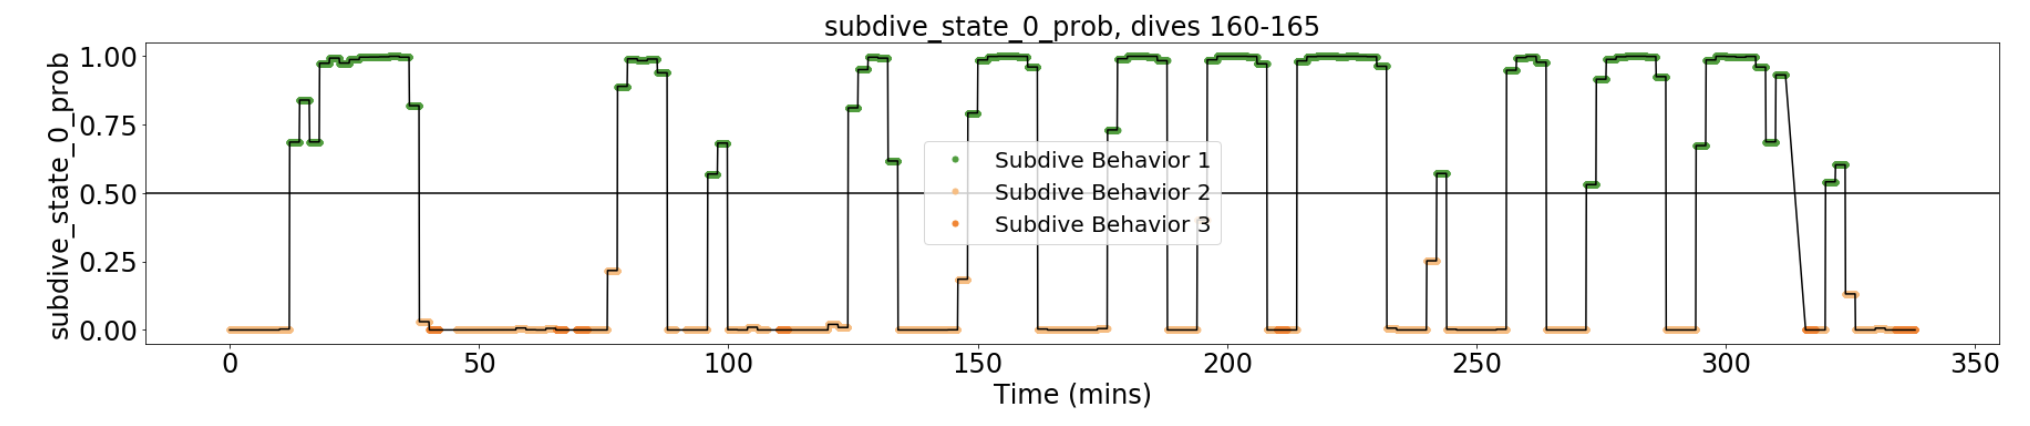
\includegraphics[width=5in]{../Plots/Fine_state_probs_1.png}
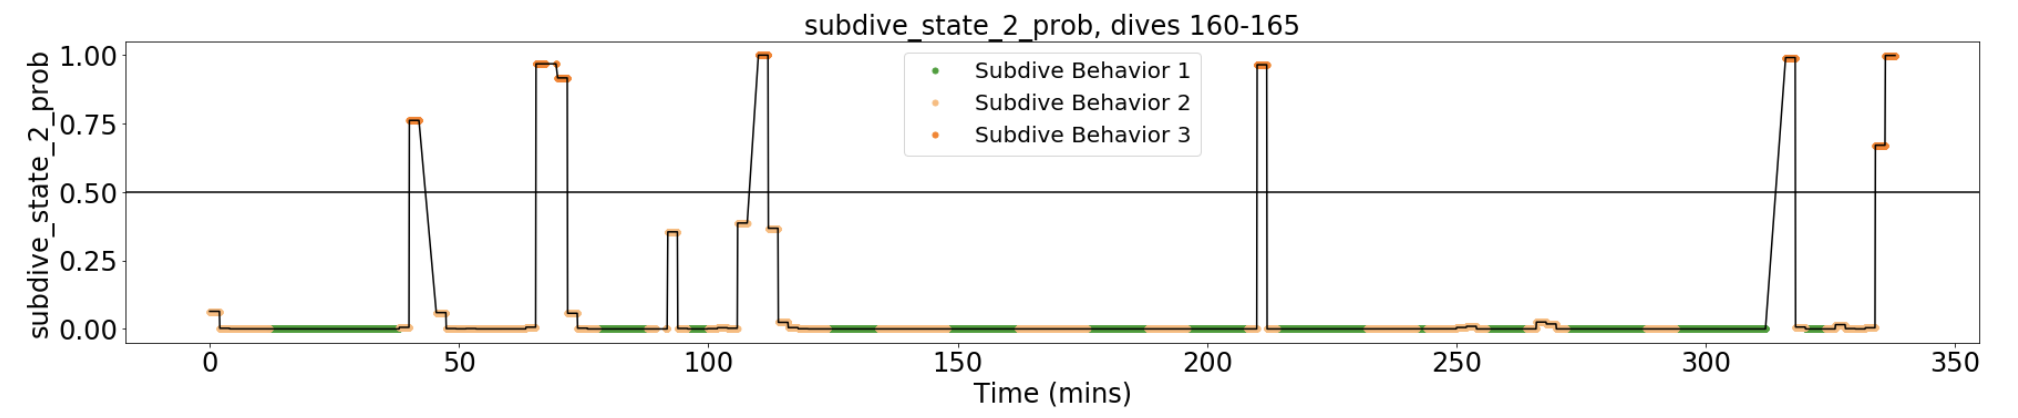
\includegraphics[width=5in]{../Plots/Fine_state_probs_3.png}

\newpage

\subsection{Model validation- empirical distributions and pseudoresiduals}
\subsubsection{Dive Duration ($Y$)}

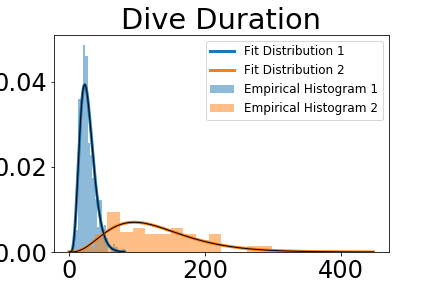
\includegraphics[width=5in]{../Plots/empirical_hist_dive_duration.png}
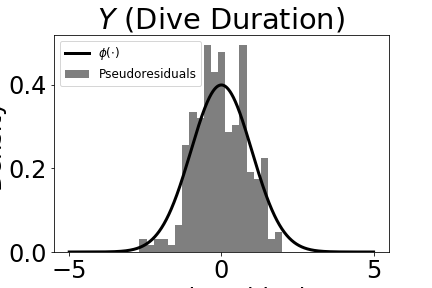
\includegraphics[width=5in]{../Plots/psedoresids_Dive_Duration.png}

\newpage
\subsubsection{Acceleration ($Z^{*(1)}$)}

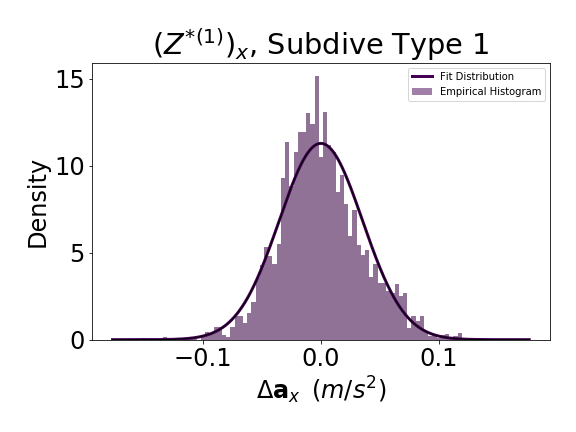
\includegraphics[width=2.5in]{../Plots/empirical_hist_Ax_0.png}
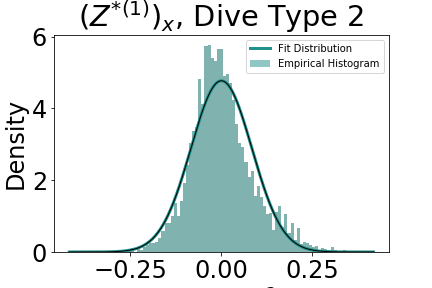
\includegraphics[width=2.5in]{../Plots/empirical_hist_Ax_1.png}
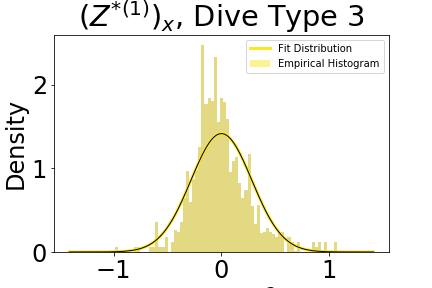
\includegraphics[width=2.5in]{../Plots/empirical_hist_Ax_2.png}
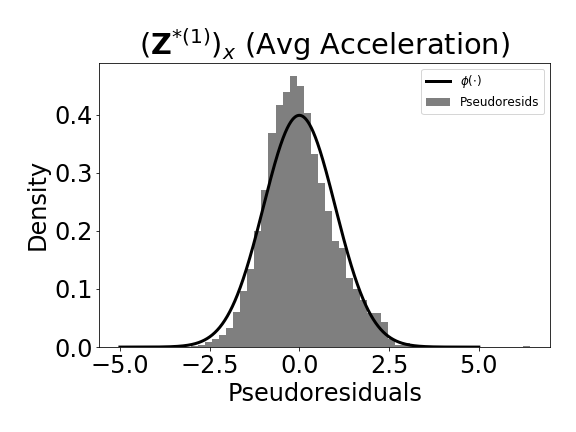
\includegraphics[width=5in]{../Plots/psedoresids_Ax.png}

\newpage

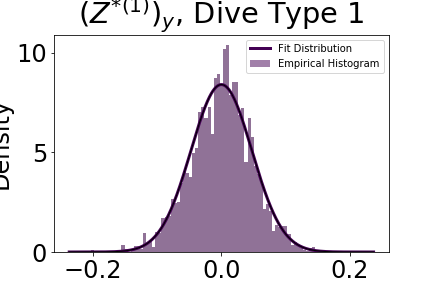
\includegraphics[width=2.5in]{../Plots/empirical_hist_Ay_0.png}
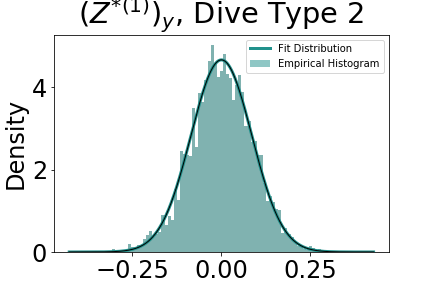
\includegraphics[width=2.5in]{../Plots/empirical_hist_Ay_1.png}
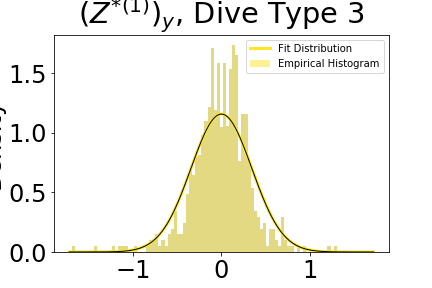
\includegraphics[width=2.5in]{../Plots/empirical_hist_Ay_2.png}
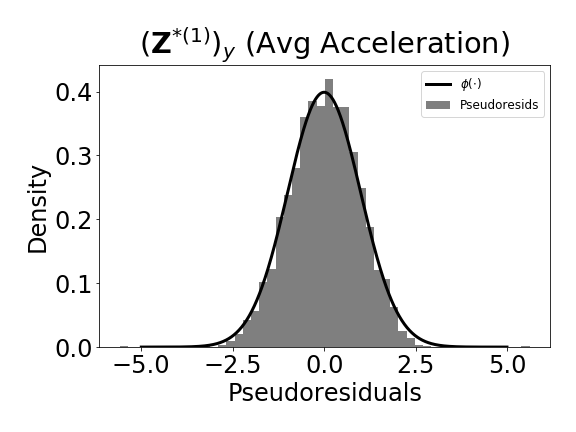
\includegraphics[width=5in]{../Plots/psedoresids_Ay.png}

\newpage

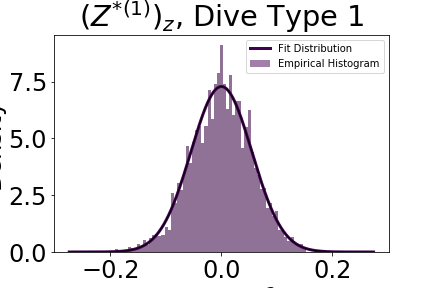
\includegraphics[width=2.5in]{../Plots/empirical_hist_Az_0.png}
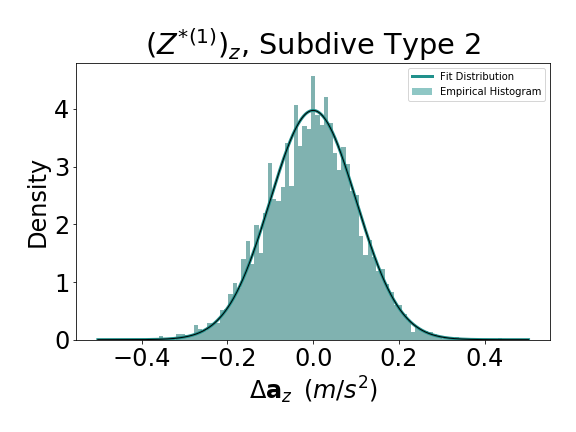
\includegraphics[width=2.5in]{../Plots/empirical_hist_Az_1.png}
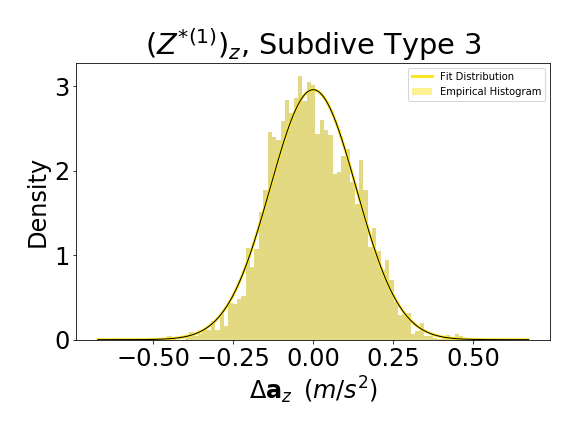
\includegraphics[width=2.5in]{../Plots/empirical_hist_Az_2.png}
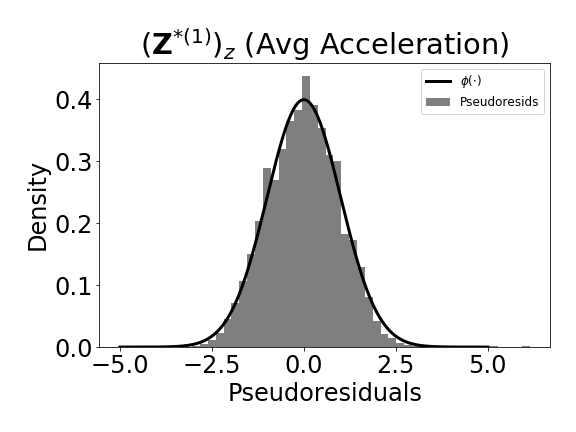
\includegraphics[width=5in]{../Plots/psedoresids_Az.png}

\newpage
\subsubsection{Fourier Sums ($Z^{*(2)}$)}

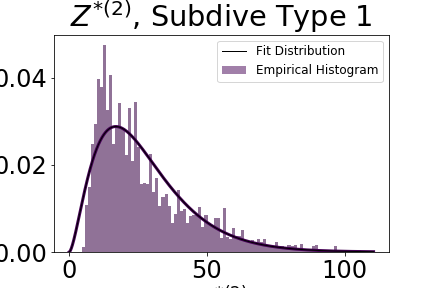
\includegraphics[width=2.5in]{../Plots/empirical_hist_ahat_0.png}
\includegraphics[width=2.5in]{../Plots/empirical_hist_ahat_1.png}
\includegraphics[width=2.5in]{../Plots/empirical_hist_ahat_2.png}
\includegraphics[width=5in]{../Plots/psedoresids_ahat.png}

\end{document}



%%%%%%%%%%%%% Everything as a figure %%%%%%%%%%%%%%%%%%%%%%%




\iffalse

Below are the empirical joint distributions of the parameter estimates from the simulation study:

\subsubsection{CarHMM-DFT}

\begin{figure}
    \centering
    \includegraphics[width=5in]{../Plots/hmm_FV_Gamma_density_0.png}
    \caption{Distribution of $\hat \Gamma^{*(1)}$ for the \textbf{CarHMM-DFT}}
\end{figure}

\begin{figure}
    \centering
    \includegraphics[width=5in]{../Plots/hmm_FV_MLE_density_dive_duration_-1_0.png}
    \caption{Distribution of Dive Duration parameter estimates for the \textbf{CarHMM-DFT}}
\end{figure}

\begin{figure}[ht]
	\centering
	\begin{subfigure}[t]{\textwidth}
        \centering
        \includegraphics[height=3in]{../Plots/hmm_FV_MLE_density_A_0_0.png}
        \caption{Sub-dive state 1}
    \end{subfigure}
    \newline
    \begin{subfigure}[t]{\textwidth}
        \centering
        \includegraphics[height=3in]{../Plots/hmm_FV_MLE_density_A_0_1.png}
        \caption{Sub-dive state 2}
    \end{subfigure}
    \caption{Distribution of $Z^{*(1)}$ parameter estimates for the \textbf{CarHMM-DFT}}
\end{figure}

\begin{figure}[ht]
	\centering
	\begin{subfigure}[t]{0.4\textwidth}
        \centering
        \includegraphics[width=2in]{../Plots/hmm_FV_MLE_density_FoVeDBA_0_0.png}
        \caption{Sub-dive state 1}
    \end{subfigure}
    %
    \begin{subfigure}[t]{0.4\textwidth}
        \centering
        \includegraphics[width=2in]{../Plots/hmm_FV_MLE_density_FoVeDBA_0_1.png}
        \caption{Sub-dive state 2}
    \end{subfigure}
    \caption{Distribution of $Z^{*(2)}$ parameter estimates for the \textbf{CarHMM-DFT}}
\end{figure}

%%%%%%%%%%%%%%%%%%%%%%%%

\subsubsection{HHMM-DFT}

\begin{figure}
    \centering
    \includegraphics[width=5in]{../Plots/hhmm_FV_uncorr_Gamma_density_-1.png}
    \caption{Distribution of $\hat \Gamma$ for the \textbf{HHMM-DFT}}
\end{figure}

\begin{figure}[ht]
	\centering
	\begin{subfigure}[t]{0.45\textwidth}
        \centering
        \includegraphics[width=2.25in]{../Plots/hhmm_FV_uncorr_Gamma_density_0.png}
        \caption{Sub-dive state 1}
    \end{subfigure}
    %
    \begin{subfigure}[t]{0.45\textwidth}
        \centering
        \includegraphics[width=2.25in]{../Plots/hhmm_FV_uncorr_Gamma_density_1.png}
        \caption{Sub-dive state 2}
    \end{subfigure}
    \caption{Distribution of $\hat \Gamma^{*}$ for the \textbf{HHMM-DFT}}
\end{figure}

\begin{figure}[ht]
	\centering
	\begin{subfigure}[t]{0.45\textwidth}
        \centering
        \includegraphics[width=2.25in]{../Plots/hhmm_FV_uncorr_MLE_density_dive_duration_-1_0.png}
        \caption{Sub-dive state 1}
    \end{subfigure}
    %
    \begin{subfigure}[t]{0.45\textwidth}
        \centering
        \includegraphics[width=2.25in]{../Plots/hhmm_FV_uncorr_MLE_density_dive_duration_-1_1.png}
        \caption{Sub-dive state 2}
    \end{subfigure}
    \caption{Distribution of $Z^{*(1)}$ parameter estimates for the \textbf{HHMM-DFT}}
\end{figure}

\begin{figure}[ht]
	\centering
	\begin{subfigure}[t]{0.45\textwidth}
        \centering
        \includegraphics[width=2.25in]{../Plots/hhmm_FV_uncorr_MLE_density_A_0_0.png}
        \caption{Sub-dive state 1}
    \end{subfigure}
    %
    \begin{subfigure}[t]{0.45\textwidth}
        \centering
        \includegraphics[width=2.25in]{../Plots/hhmm_FV_uncorr_MLE_density_A_0_1.png}
        \caption{Sub-dive state 2}
    \end{subfigure}
    \caption{Distribution of $Z^{*(1)}$ parameter estimates for the \textbf{HHMM-DFT}}
\end{figure}

\begin{figure}[ht]
	\centering
	\begin{subfigure}[t]{0.45\textwidth}
        \centering
        \includegraphics[width=2.25in]{../Plots/hhmm_FV_uncorr_MLE_density_FoVeDBA_0_0.png}
        \caption{Sub-dive state 1}
    \end{subfigure}
    %
    \begin{subfigure}[t]{0.45\textwidth}
        \centering
        \includegraphics[width=2.25in]{../Plots/hhmm_FV_uncorr_MLE_density_FoVeDBA_0_1.png}
        \caption{Sub-dive state 2}
    \end{subfigure}
    \caption{Distribution of $Z^{*(2)}$ parameter estimates for the \textbf{HHMM-DFT}}
\end{figure}

%%%%%%%%%%%%%%%%%%%%%%%%%%%%%%%%%

\subsubsection{CarHHMM}

\begin{figure}
    \centering
    \includegraphics[width=5in]{../Plots/hhmm_V_Gamma_density_-1.png}
    \caption{Distribution of $\hat \Gamma$ for the \textbf{CarHHMM}}
\end{figure}

\begin{figure}[ht]
	\centering
	\begin{subfigure}[t]{0.45\textwidth}
        \centering
        \includegraphics[width=2.25in]{../Plots/hhmm_V_Gamma_density_0.png}
        \caption{Sub-dive state 1}
    \end{subfigure}
    %
    \begin{subfigure}[t]{0.45\textwidth}
        \centering
        \includegraphics[width=2.25in]{../Plots/hhmm_V_Gamma_density_1.png}
        \caption{Sub-dive state 2}
    \end{subfigure}
    \caption{Distribution of $\hat \Gamma^{*}$ for the \textbf{CarHHMM}}
\end{figure}

\begin{figure}[ht]
	\centering
	\begin{subfigure}[t]{0.45\textwidth}
        \centering
        \includegraphics[width=2.25in]{../Plots/hhmm_V_MLE_density_dive_duration_-1_0.png}
        \caption{Sub-dive state 1}
    \end{subfigure}
    %
    \begin{subfigure}[t]{0.45\textwidth}
        \centering
        \includegraphics[width=2.25in]{../Plots/hhmm_V_MLE_density_dive_duration_-1_1.png}
        \caption{Sub-dive state 2}
    \end{subfigure}
    \caption{Distribution of $Z^{*(1)}$ parameter estimates for the \textbf{CarHHMM}}
\end{figure}

\begin{figure}[ht]
	\centering
	\begin{subfigure}[t]{\textwidth}
        \centering
        \includegraphics[height=3in]{../Plots/hhmm_V_MLE_density_A_0_0.png}
        \caption{Sub-dive state 1}
    \end{subfigure}
    \newline
    \begin{subfigure}[t]{\textwidth}
        \centering
        \includegraphics[height=3in]{../Plots/hhmm_V_MLE_density_A_0_1.png}
        \caption{Sub-dive state 2}
    \end{subfigure}
    \caption{Distribution of $Z^{*(1)}$ parameter estimates for the \textbf{CarHHMM}}
\end{figure}

\subsubsection{CarHHMM-DFT}

\begin{figure}
    \centering
    \includegraphics[width=5in]{../Plots/hhmm_FV_Gamma_density_-1.png}
    \caption{Distribution of $\hat \Gamma$ for the \textbf{CarHHMM-DFT}}
\end{figure}

\begin{figure}[ht]
	\centering
	\begin{subfigure}[t]{0.45\textwidth}
        \centering
        \includegraphics[width=2.25in]{../Plots/hhmm_FV_Gamma_density_0.png}
        \caption{Sub-dive state 1}
    \end{subfigure}
    %
    \begin{subfigure}[t]{0.45\textwidth}
        \centering
        \includegraphics[width=2.25in]{../Plots/hhmm_FV_Gamma_density_1.png}
        \caption{Sub-dive state 2}
    \end{subfigure}
    \caption{Distribution of $\hat \Gamma^{*}$ for the \textbf{CarHHMM-DFT}}
\end{figure}

\begin{figure}[ht]
	\centering
	\begin{subfigure}[t]{0.45\textwidth}
        \centering
        \includegraphics[width=2.25in]{../Plots/hhmm_FV_MLE_density_dive_duration_-1_0.png}
        \caption{Sub-dive state 1}
    \end{subfigure}
    %
    \begin{subfigure}[t]{0.45\textwidth}
        \centering
        \includegraphics[width=2.25in]{../Plots/hhmm_FV_MLE_density_dive_duration_-1_1.png}
        \caption{Sub-dive state 2}
    \end{subfigure}
    \caption{Distribution of $Z^{*(1)}$ parameter estimates for the \textbf{CarHHMM-DFT}}
\end{figure}

\begin{figure}[ht]
	\centering
	\begin{subfigure}[t]{\textwidth}
        \centering
        \includegraphics[height=3in]{../Plots/hhmm_FV_MLE_density_A_0_0.png}
        \caption{Sub-dive state 1}
    \end{subfigure}
    \newline
    \begin{subfigure}[t]{\textwidth}
        \centering
        \includegraphics[height=3in]{../Plots/hhmm_FV_MLE_density_A_0_1.png}
        \caption{Sub-dive state 2}
    \end{subfigure}
    \caption{Distribution of $Z^{*(1)}$ parameter estimates for the \textbf{CarHHMM-DFT}}
\end{figure}

\begin{figure}[ht]
	\centering
	\begin{subfigure}[t]{0.45\textwidth}
        \centering
        \includegraphics[width=2.25in]{../Plots/hhmm_FV_MLE_density_FoVeDBA_0_0.png}
        \caption{Sub-dive state 1}
    \end{subfigure}
    %
    \begin{subfigure}[t]{0.45\textwidth}
        \centering
        \includegraphics[width=2.25in]{../Plots/hhmm_FV_MLE_density_FoVeDBA_0_1.png}
        \caption{Sub-dive state 2}
    \end{subfigure}
    \caption{Distribution of $Z^{*(2)}$ parameter estimates for the \textbf{CarHHMM-DFT}}
\end{figure}

%%% Accuracy %%%

\begin{table}
\centering
\caption{Accuracies and run times for all models. All reported values are averages, and $\pm$ refers to the standard deviation.}
\scalebox{0.8}{
\begin{tabular}{ccccccc}
Model                      & \multicolumn{1}{c}{Training Time (Minutes)} & \multicolumn{1}{c}{Dive Type} & \multicolumn{1}{c}{Subdive Type} & \multicolumn{1}{c}{Dive Accuracy} & \multicolumn{1}{c}{Subdive Accuracy}  \\ \hline
\multirow{5}{*}{CarHMM-DFT}& \multirow{5}{*}{$15.74 \pm 2.46$}   & Both                          & Both                             & -------------                     & $1.00 \pm 0.00$                       \\
                           &                                    & 1                             & 1                                & \multirow{2}{*}{-------------}    & $1.00 \pm 0.00$                       \\ 
                           &                                    & 1                             & 2                                &                                   & $1.00 \pm 0.00$                       \\ 
                           &                                    & 2                             & 1                                & \multirow{2}{*}{-------------}    & $1.00 \pm 0.00$                       \\ 
                           &                                    & 2                             & 2                                &                                   & $1.00 \pm 0.00$                       \\ \hline 
\multirow{5}{*}{HHMM-DFT}  & \multirow{5}{*}{$82.43 \pm 11.48$}   & Both                          & Both                             & $0.94 \pm 0.02$                   & $1.00 \pm 0.00$                       \\
                           &                                    & 1                             & 1                                & \multirow{2}{*}{$0.94\pm0.03$}    & $1.00 \pm 0.00$                       \\ 
                           &                                    & 1                             & 2                                &                                   & $1.00 \pm 0.00$                       \\ 
                           &                                    & 2                             & 1                                & \multirow{2}{*}{$0.94\pm0.03$}    & $1.00 \pm 0.00$                       \\ 
                           &                                    & 2                             & 2                                &                                   & $1.00 \pm 0.00$                       \\ \hline
\multirow{5}{*}{CarHHMM}   & \multirow{5}{*}{$70.85 \pm 15.89$}   & Both                          & Both                             & $0.91 \pm 0.03$                   & $0.89 \pm 0.02$                       \\
                           &                                    & 1                             & 1                                & \multirow{2}{*}{$0.87\pm0.04$}    & $0.44 \pm 0.12$                       \\ 
                           &                                    & 1                             & 2                                &                                   & $1.00 \pm 0.00$                       \\ 
                           &                                    & 2                             & 1                                & \multirow{2}{*}{$0.95\pm0.03$}    & $0.81 \pm 0.04$                       \\ 
                           &                                    & 2                             & 2                                &                                   & $1.00 \pm 0.00$                       \\ \hline
\multirow{5}{*}{CarHHMM-DFT}& \multirow{5}{*}{$81.22 \pm 16.10$}   & Both                          & Both                             & $0.94 \pm 0.02$                   & $1.00 \pm 0.00$                       \\
                           &                                    & 1                             & 1                                & \multirow{2}{*}{$0.94\pm0.03$}    & $1.00 \pm 0.00$                       \\ 
                           &                                    & 1                             & 2                                &                                   & $1.00 \pm 0.00$                       \\ 
                           &                                    & 2                             & 1                                & \multirow{2}{*}{$0.94\pm0.03$}    & $1.00 \pm 0.00$                       \\ 
                           &                                    & 2                             & 2                                &                                   & $1.00 \pm 0.00$                       \\ \hline
\end{tabular}
}
\label{table:accuracy}
\end{table}


%%% dive duration %%%

\begin{table}
\centering
\caption{Estimates and standard errors of parameters for dive duration distribution for all four models. All reported values are averages, except for the Fisher observed standard error, which are medians. $\pm$ refers to the IQR.}
\scalebox{0.9}{
\begin{tabular}{ccccccc}
Model                      & \multicolumn{1}{c}{Parameter} & \multicolumn{1}{c}{Dive Type} & \multicolumn{1}{c}{Estimate} & \multicolumn{1}{c}{Bias} & \multicolumn{1}{c}{Empirical SE} & \multicolumn{1}{c}{Observed Fischer SE}           \\ \hline
\multirow{4}{*}{CarHMM-DFT}& \multirow{2}{*}{$\mu$}        & 1                             & $49.72$                         & $-0.28$                     & $4.78$                             & $2.47 \pm 0.34$                             \\
                           &                               & ---                           & ---                            & ---                        & ---                                & ---                                         \\
                           & \multirow{2}{*}{$\sigma$}     & 1                             & $39.00$                         & $-7.51$                     & $5.05$                             & $2.50 \pm 0.40$                             \\
                           &                               & ---                           & ---                            & ---                        & ---                                & ---                                         \\ \hline
\multirow{4}{*}{HHMM-DFT}  & \multirow{2}{*}{$\mu$}        & 1                             & $19.99$                         & $-0.01$                     & $0.75$                             & $0.69 \pm 0.11$                             \\
                           &                               & 2                             & $79.85$                         & $-0.15$                     & $8.05$                             & $5.85 \pm 1.10$                             \\
                           & \multirow{2}{*}{$\sigma$}     & 1                             & $4.90$                         & $-0.10$                     & $0.61$                             & $0.53 \pm 0.10$                             \\
                           &                               & 2                             & $48.74$                         & $-1.26$                     & $6.50$                             & $5.15 \pm 1.02$                             \\ \hline
\multirow{4}{*}{CarHHMM}   & \multirow{2}{*}{$\mu$}        & 1                             & $19.91$                         & $-0.09$                     & $0.77$                             & $0.71 \pm 0.12$                             \\
                           &                               & 2                             & $75.80$                         & $-4.20$                     & $7.72$                             & $5.32 \pm 0.98$                             \\
                           & \multirow{2}{*}{$\sigma$}     & 1                             & $4.73$                         & $-0.27$                     & $0.59$                             & $0.55 \pm 0.10$                             \\
                           &                               & 2                             & $49.48$                         & $-0.52$                     & $6.26$                             & $4.79 \pm 0.93$                             \\ \hline
\multirow{4}{*}{CarHHMM-DFT}& \multirow{2}{*}{$\mu$}        & 1                             & $19.99$                         & $-0.01$                     & $0.75$                             & $0.69 \pm 0.12$                             \\
                           &                               & 2                             & $79.85$                         & $-0.15$                     & $8.05$                             & $5.85 \pm 1.10$                             \\
                           & \multirow{2}{*}{$\sigma$}     & 1                             & $4.90$                         & $-0.10$                     & $0.61$                             & $0.53 \pm 0.10$                             \\
                           &                               & 2                             & $48.74$                         & $-1.26$                     & $6.50$                             & $5.15 \pm 1.02$                             
\end{tabular}
}
\label{table:dive_duration}
\end{table}

%%% Acceleration %%%

\begin{table}
\centering
\caption{Estimates and standard errors of parameters for $Z^{*(1)}_{t,t^*}$ for all four models. All reported values are averages, except for the Fisher observed standard error, which are medians. $\pm$ refers to the IQR.}
\scalebox{0.7}{
\begin{tabular}{ccccccc}
Model                      & \multicolumn{1}{c}{Parameter} & \multicolumn{1}{c}{Subdive Type} & \multicolumn{1}{c}{Estimate} & \multicolumn{1}{c}{Bias} & \multicolumn{1}{c}{Empirical SE} & \multicolumn{1}{c}{Observed Fischer SE}        \\ \hline
\multirow{6}{*}{CarHMM-DFT}& \multirow{2}{*}{$\mu$}        & 1                             & $0.00$                         & $0.00$                     & $0.00$                             & $0.14 \pm 0.13$                             \\
                           &                               & 2                             & $0.00$                         & $0.00$                     & $0.01$                             & $0.06 \pm 0.02$                             \\
                           & \multirow{2}{*}{$\sigma$}     & 1                             & $0.05$                         & $-0.00$                     & $0.00$                             & $0.00 \pm 0.00$                             \\
                           &                               & 2                             & $0.10$                         & $-0.00$                     & $0.00$                             & $0.00 \pm 0.00$                             \\ 
                           & \multirow{2}{*}{$\phi$}       & 1                             & $0.99$                         & $-0.00$                     & $0.01$                             & $0.01 \pm 0.00$                             \\
                           &                               & 2                             & $0.95$                         & $-0.00$                     & $0.01$                             & $0.01 \pm 0.00$                             \\ \hline
\multirow{6}{*}{HHMM-DFT}  & \multirow{2}{*}{$\mu$}        & 1                             & $-0.01$                         & $-0.01$                     & $0.02$                             & $0.01 \pm 0.00$                             \\
                           &                               & 2                             & $-0.00$                         & $-0.00$                     & $0.02$                             & $0.01 \pm 0.00$                             \\
                           & \multirow{2}{*}{$\sigma$}     & 1                             & $0.25$                         & $0.20$                     & $0.04$                             & $0.00 \pm 0.00$                             \\
                           &                               & 2                             & $0.24$                         & $0.14$                     & $0.03$                             & $0.00 \pm 0.00$                             \\ 
                           & \multirow{2}{*}{$\phi$}       & 1                             & ------                         & ------                     & ------                             & ------                                      \\
                           &                               & 2                             & ------                         & ------                     & ------                             & ------                                      \\ \hline
\multirow{6}{*}{CarHHMM}   & \multirow{2}{*}{$\mu$}        & 1                             & $0.00$                         & $0.00$                     & $0.00$                             & $0.08 \pm 0.04$                             \\
                           &                               & 2                             & $-0.01$                         & $-0.01$                     & $0.01$                             & $0.01 \pm 0.00$                             \\
                           & \multirow{2}{*}{$\sigma$}     & 1                             & $0.05$                         & $0.00$                     & $0.04$                             & $0.00 \pm 0.00$                             \\
                           &                               & 2                             & $0.27$                         & $0.17$                     & $0.01$                             & $0.00 \pm 0.00$                             \\ 
                           & \multirow{2}{*}{$\phi$}       & 1                             & $0.97$                         & $-0.02$                     & $0.10$                             & $0.00 \pm 0.00$                             \\
                           &                               & 2                             & $0.49$                         & $-0.46$                     & $0.05$                             & $0.02 \pm 0.00$                             \\ \hline
\multirow{6}{*}{CarHHMM-DFT}& \multirow{2}{*}{$\mu$}        & 1                             & $0.00$                         & $0.00$                     & $0.00$                             & $0.13 \pm 0.12$                             \\
                           &                               & 2                             & $0.00$                         & $0.00$                     & $0.00$                             & $0.06 \pm 0.02$                             \\
                           & \multirow{2}{*}{$\sigma$}     & 1                             & $0.05$                         & $-0.00$                     & $0.00$                             & $0.00 \pm 0.00$                             \\
                           &                               & 2                             & $0.10$                         & $-0.00$                     & $0.00$                             & $0.00 \pm 0.00$                             \\ 
                           & \multirow{2}{*}{$\phi$}       & 1                             & $0.99$                         & $-0.00$                     & $0.01$                             & $0.01 \pm 0.00$                             \\
                           &                               & 2                             & $0.95$                         & $-0.00$                     & $0.01$                             & $0.01 \pm 0.00$                             \\ \hline
\end{tabular}
}
\label{table:acceleration}
\end{table}


%%% FoVeDBA %%%

\begin{table}
\centering
\caption{Estimates and standard errors of parameters for $Z^{*(2)}_{t,t^*}$ for all four models. All reported values are averages, except for the Fisher observed standard error, which are medians. $\pm$ refers to the IQR.}
\scalebox{0.8}{
\begin{tabular}{ccccccc}
Model                      & \multicolumn{1}{c}{Parameter} & \multicolumn{1}{c}{Subdive Type} & \multicolumn{1}{c}{Estimate} & \multicolumn{1}{c}{Bias} & \multicolumn{1}{c}{Empirical SE} & \multicolumn{1}{c}{Observed Fischer SE}        \\ \hline
\multirow{4}{*}{CarHMM-DFT}& \multirow{2}{*}{$\mu$}        & 1                             & $10.10$                         & $-0.00$                     & $0.09$                             & $0.08 \pm 0.01$                             \\
                           &                               & 2                             & $305.97$                         & $0.03$                     & $0.54$                             & $0.51 \pm 0.03$                             \\
                           & \multirow{2}{*}{$\sigma$}     & 1                             & $3.18$                         & $-0.00$                     & $0.07$                             & $0.06 \pm 0.01$                             \\
                           &                               & 2                             & $17.46$                         & $-0.03$                     & $0.37$                             & $0.36 \pm 0.02$                             \\ \hline
\multirow{4}{*}{HHMM-DFT}  & \multirow{2}{*}{$\mu$}        & 1                             & $10.10$                         & $-0.00$                     & $0.09$                             & $0.08 \pm 0.01$                             \\
                           &                               & 2                             & $305.97$                         & $0.03$                     & $0.54$                             & $0.51 \pm 0.03$                             \\
                           & \multirow{2}{*}{$\sigma$}     & 1                             & $3.18$                         & $-0.00$                     & $0.07$                             & $0.06 \pm 0.01$                             \\
                           &                               & 2                             & $17.46$                         & $-0.03$                     & $0.37$                             & $0.36 \pm 0.02$                             \\ \hline
\multirow{4}{*}{CarHHMM}   & \multirow{2}{*}{$\mu$}        & 1                             & ------                         & ------                     & ------                             & ------                                      \\
                           &                               & 2                             & ------                         & ------                     & ------                             & ------                                      \\
                           & \multirow{2}{*}{$\sigma$}     & 1                             & ------                         & ------                     & ------                             & ------                                      \\
                           &                               & 2                             & ------                         & ------                     & ------                             & ------                                      \\ \hline
\multirow{4}{*}{CarHHMM-DFT}& \multirow{2}{*}{$\mu$}        & 1                             & $10.10$                         & $-0.00$                     & $0.09$                             & $0.08 \pm 0.01$                             \\
                           &                               & 2                             & $305.97$                         & $0.03$                     & $0.54$                             & $0.51 \pm 0.03$                             \\
                           & \multirow{2}{*}{$\sigma$}     & 1                             & $3.18$                         & $-0.00$                     & $0.07$                             & $0.06 \pm 0.01$                             \\
                           &                               & 2                             & $17.46$                         & $-0.03$                     & $0.37$                             & $0.36 \pm 0.02$                             
\end{tabular}
}
\label{table:FoVeDBA}
\end{table}

% Gamma
\begin{table}[t]
\centering
\caption{Estimates and standard errors of $\Gamma$ and $\Gamma^*$ for all four models. All reported values are averages except for the observed fisher SE, which is a median. $\pm$ refers to the IQR.}
\scalebox{0.7}{
\begin{tabular}{ccccccc}
Model                        & \multicolumn{1}{c}{Parameter} & \multicolumn{1}{c}{Estimate}   & \multicolumn{1}{c}{Bias} & \multicolumn{1}{c}{Empirical SE} & \multicolumn{1}{c}{Observed Fischer SE}     \\ \hline
\multirow{6}{*}{HHMM-DFT}    & $\Gamma_{12}$                 & $0.50$                         & $-0.00$                   & $0.03$                           & $0.08 \pm 0.01$                             \\
                             & $\Gamma_{21}$                 & $0.50$                         & $-0.00$                   & $0.03$                           & $0.08 \pm 0.01$                             \\
                             & $\Gamma^{*(1)}_{12}$          & $0.50$                         & $0.00$                   & $0.00$                           & $0.07 \pm 0.01$                             \\
                             & $\Gamma^{*(1)}_{21}$          & $0.10$                         & $0.00$                   & $0.02$                           & $0.02 \pm 0.00$                             \\
                             & $\Gamma^{*(2)}_{12}$          & $0.20$                         & $-0.00$                   & $0.01$                           & $0.01 \pm 0.00$                             \\
                             & $\Gamma^{*(2)}_{21}$          & $0.30$                         & $-0.00$                   & $0.02$                           & $0.02 \pm 0.00$                             \\ \hline
\multirow{6}{*}{CarHMM-DFT}  & $\Gamma_{12}$                 & ------                         & ------                   & ------                           & ------                                      \\
                             & $\Gamma_{21}$                 & ------                         & ------                   & ------                           & ------                                      \\
                             & $\Gamma^{*(1)}_{12}$          & $0.23$                         & ------                   & $0.01$                           & $0.00 \pm 0.00$                             \\
                             & $\Gamma^{*(1)}_{21}$          & $0.23$                         & ------                   & $0.02$                           & $0.00 \pm 0.00$                             \\
                             & $\Gamma^{*(2)}_{12}$          & ------                         & ------                   & ------                           & ------                                      \\
                             & $\Gamma^{*(2)}_{21}$          & ------                         & ------                   & ------                           & ------                                      \\ \hline
\multirow{6}{*}{CarHHMM}     & $\Gamma_{12}$                 & $0.49$                         & $-0.01$                   & $0.02$                           & $0.08 \pm 0.01$                             \\
                             & $\Gamma_{21}$                 & $0.50$                         & $0.00$                   & $0.02$                           & $0.08 \pm 0.01$                             \\
                             & $\Gamma^{*(1)}_{12}$          & $0.50$                         & $-0.00$                   & $0.00$                           & $0.23 \pm 0.19$                             \\
                             & $\Gamma^{*(1)}_{21}$          & $0.04$                         & $-0.06$                   & $0.02$                           & $0.01 \pm 0.00$                             \\
                             & $\Gamma^{*(2)}_{12}$          & $0.11$                         & $-0.09$                   & $0.02$                           & $0.01 \pm 0.00$                             \\
                             & $\Gamma^{*(2)}_{21}$          & $0.11$                         & $-0.19$                   & $0.03$                           & $0.01 \pm 0.00$                             \\ \hline
\multirow{6}{*}{CarHHMM-DFT} & $\Gamma_{12}$                 & $0.50$                         & $-0.00$                   & $0.03$                           & $0.08 \pm 0.01$                             \\
                             & $\Gamma_{21}$                 & $0.50$                         & $-0.00$                   & $0.03$                           & $0.08 \pm 0.01$                             \\
                             & $\Gamma^{*(1)}_{12}$          & $0.50$                         & $0.00$                   & $0.00$                           & $0.07 \pm 0.01$                             \\
                             & $\Gamma^{*(1)}_{21}$          & $0.10$                         & $0.00$                   & $0.02$                           & $0.02 \pm 0.00$                             \\
                             & $\Gamma^{*(2)}_{12}$          & $0.20$                         & $-0.00$                   & $0.01$                           & $0.01 \pm 0.00$                             \\
                             & $\Gamma^{*(2)}_{21}$          & $0.30$                         & $-0.00$                   & $0.02$                           & $0.02 \pm 0.00$                             \\ \hline

\end{tabular}
}
\label{table:Gamma}
\end{table}

\section{Case Study Results}

\subsection{Model selection- lag plots}

\begin{figure}[ht]
	\centering
	\includegraphics[height=7in]{../Plots/lagplot.png}
	\caption{Lag plots of all features on both the fine- and coarse- scale.}
	\label{fig:lag}
\end{figure}

\subsection{Results- decoded state probabilities}

\begin{figure}[ht]
	\centering
	\includegraphics[width=5in]{../Plots/Coarse_state_probs.png}
	\caption{Probabilities of dive types for the set of 5 killer whale dives.}
	\label{fig:coarse_probs}
\end{figure}
%
\begin{figure}[ht]
	\centering
	\begin{subfigure}[t]{1.0\textwidth}
        \centering
        \includegraphics[width=5in]{../Plots/Fine_state_probs_1.png}
        \caption{Fine-scale state 1 probabilities}
    \end{subfigure}
    \newline
    \begin{subfigure}[t]{1.0\textwidth}
        \centering
        \includegraphics[width=5in]{../Plots/Fine_state_probs_3.png}
        \caption{Fine-scale state 3 probabilities}
    \end{subfigure}
	\caption{Probabilities of sub-dive types for the set of 5 killer whale dives.}
	\label{fig:fine_probs}
\end{figure}

\subsection{Model validation- empirical distributions and pseudoresiduals}

\subsubsection{Dive Duration ($Y$)}

\begin{figure}
    \centering
    \includegraphics[width=5in]{../Plots/empirical_hist_dive_duration.png}
    \caption{Empirical distribution of dive duration observations vs the fitted PDF}
\end{figure}

\begin{figure}
    \centering
    \includegraphics[width=5in]{../Plots/psedoresids_Dive_Duration.png}
    \caption{Pseudoresiduals of dive duration observations}
\end{figure}

\subsubsection{Acceleration ($Z^{*(1)}$)}

%% Ax %%

\begin{figure}[ht]
	\centering
	\begin{subfigure}[t]{0.3\textwidth}
        \centering
        \includegraphics[width=1.5in]{../Plots/empirical_hist_Ax_0.png}
        \caption{Sub-dive state 1}
    \end{subfigure}
    %
    \begin{subfigure}[t]{0.3\textwidth}
        \centering
        \includegraphics[width=1.5in]{../Plots/empirical_hist_Ax_1.png}
        \caption{Sub-dive state 2}
    \end{subfigure}
    %
    \begin{subfigure}[t]{0.3\textwidth}
        \centering
        \includegraphics[width=1.5in]{../Plots/empirical_hist_Ax_2.png}
        \caption{Sub-dive state 3}
    \end{subfigure}
    \caption{Empirical distribution of $\left(Z^{*(1)}\right)_x$ observations vs the fitted PDF}
\end{figure}

\begin{figure}
    \centering
    \includegraphics[width=5in]{../Plots/psedoresids_Ax.png}
    \caption{Pseudoresiduals of $\left(Z^{*(1)}\right)_x$ observations}
\end{figure}

%% Ay %%

\begin{figure}[ht]
	\centering
	\begin{subfigure}[t]{0.3\textwidth}
        \centering
        \includegraphics[width=1.5in]{../Plots/empirical_hist_Ay_0.png}
        \caption{Sub-dive state 1}
    \end{subfigure}
    %
    \begin{subfigure}[t]{0.3\textwidth}
        \centering
        \includegraphics[width=1.5in]{../Plots/empirical_hist_Ay_1.png}
        \caption{Sub-dive state 2}
    \end{subfigure}
    %
    \begin{subfigure}[t]{0.3\textwidth}
        \centering
        \includegraphics[width=1.5in]{../Plots/empirical_hist_Ay_2.png}
        \caption{Sub-dive state 3}
    \end{subfigure}
    \caption{Empirical distribution of $\left(Z^{*(1)}\right)_y$ observations vs the fitted PDF}
\end{figure}

\begin{figure}
    \centering
    \includegraphics[width=5in]{../Plots/psedoresids_Ay.png}
    \caption{Pseudoresiduals of $\left(Z^{*(1)}\right)_y$ observations}
\end{figure}

%% Az %%

\begin{figure}[ht]
	\centering
	\begin{subfigure}[t]{0.3\textwidth}
        \centering
        \includegraphics[width=1.5in]{../Plots/empirical_hist_Az_0.png}
        \caption{Sub-dive state 1}
    \end{subfigure}
    %
    \begin{subfigure}[t]{0.3\textwidth}
        \centering
        \includegraphics[width=1.5in]{../Plots/empirical_hist_Az_1.png}
        \caption{Sub-dive state 2}
    \end{subfigure}
    %
    \begin{subfigure}[t]{0.3\textwidth}
        \centering
        \includegraphics[width=1.5in]{../Plots/empirical_hist_Az_2.png}
        \caption{Sub-dive state 3}
    \end{subfigure}
    \caption{Empirical distribution of $\left(Z^{*(1)}\right)_z$ observations vs the fitted PDF}
\end{figure}

\begin{figure}
    \centering
    \includegraphics[width=5in]{../Plots/psedoresids_Az.png}
    \caption{Pseudoresiduals of $\left(Z^{*(1)}\right)_z$ observations}
\end{figure}

\subsubsection{Fourier Sums ($Z^{*(2)}$)}

\begin{figure}[ht]
	\centering
	\begin{subfigure}[t]{0.3\textwidth}
        \centering
        \includegraphics[width=1.5in]{../Plots/empirical_hist_ahat_0.png}
        \caption{Sub-dive state 1}
    \end{subfigure}
    %
    \begin{subfigure}[t]{0.3\textwidth}
        \centering
        \includegraphics[width=1.5in]{../Plots/empirical_hist_ahat_1.png}
        \caption{Sub-dive state 2}
    \end{subfigure}
    %
    \begin{subfigure}[t]{0.3\textwidth}
        \centering
        \includegraphics[width=1.5in]{../Plots/empirical_hist_ahat_2.png}
        \caption{Sub-dive state 3}
    \end{subfigure}
    \caption{Empirical distribution of $Z^{*(2)}$ observations vs the fitted PDF}
\end{figure}

\begin{figure}
    \centering
    \includegraphics[width=5in]{../Plots/psedoresids_ahat.png}
    \caption{Pseudoresiduals of $Z^{*(2)}$ observations}
\end{figure}

\end{document}


\fi